\pdfinfo{
    /Author (Francesco Biscaccia Carrara)
    /Title (Enhancing the ACS Heuristic: Parameter Tuning and Computational Experiments for Solving MIP Problems)
    /Subject (Master Degree thesis in Computer Engineering UniPD 2024/2025)
    /Keyword (ACS, Heuristic, MIP, Parallelism, MIPLIB2017)
}

% Libraries
\documentclass[a4paper,12pt,ì]{report}
%\documentclass[a4paper,12pt,twoside]{report} solo per stampa
\usepackage[utf8]{inputenc}
\usepackage{bookmark}
\usepackage{hyperref}
\usepackage[english]{babel}
\usepackage{fancyhdr}%%%%%%%%%%
\usepackage{sectsty}
\usepackage[inner=3cm,top=2cm,bottom=2cm,outer=2cm]{geometry}
\usepackage{setspace}
\usepackage[hang,small,sf,font=small, labelfont=bf]{caption}
\usepackage{subcaption}
\usepackage{graphicx}
\graphicspath{{./chapter/img/}}
\usepackage[usenames]{color}
\usepackage{amsmath,amssymb}
\usepackage{xcolor}
\usepackage{colortbl}
\usepackage{tocloft}
\usepackage[a-1b]{pdfx}
\usepackage{algorithm}
\usepackage{algpseudocode}
\usepackage{hyperref}
\usepackage{tabto}
\usepackage{pgfplots}

\usepackage{tikz}
\usepackage{circuitikz}

\usepackage{bbold}

\usepackage{amsmath}
\usepackage{amsthm}


\DeclareMathOperator{\E}{\mathbb{E}}
\DeclareMathOperator{\Prob}{\mathbb{P}}
%-------------TO REMOVE------------
\newtheorem{definition}{Definition} %
\newtheorem{theorem}{Teorema} %
\newtheorem{problem}{Problema} %
%-----------------------------------
\usetikzlibrary{patterns}
\usetikzlibrary{math}
\pgfplotsset{width=10cm,compat=1.9}


\usepackage{indentfirst}
\setlength{\arrayrulewidth}{1pt}
\usepackage{afterpage}
\newcommand\blankpage{%
    \null%
    \thispagestyle{empty}%
    \addtocounter{page}{-1}%
    \newpage}

% Mandatory settings
\onehalfspacing%
\hypersetup{
    colorlinks,
    citecolor=black,
    filecolor=black,
    linkcolor=black,
    urlcolor=black,
    pdfpagelabels
}

% Subsections
\renewcommand{\cftpartleader}{\cftdotfill{\cftdotsep}} % for parts
\renewcommand{\cftchapleader}{\cftdotfill{\cftdotsep}} % for chapters
\renewcommand{\cftsecleader}{\cftdotfill{\cftdotsep}} % for sections


%\pagestyle{fancy}
%\renewcommand{\chaptermark}[1]{\markboth{\chaptername\ \thechapter.\ #1 }{}}
%\renewcommand{\sectionmark}[1]{\markright{\thesection\ #1}{}}
%\fancyhead{}
%\fancyhead[LE,RO]{\sffamily \thepage}
%\fancyhead[RE]{\sffamily \leftmark}
%\fancyhead[LO]{\sffamily \rightmark}
%\fancyfoot{}

%\fancypagestyle{plain}{ \fancyhead{} \fancyfoot{}
%\fancyfoot[C]{\sffamily \thepage}
%\renewcommand{\headrulewidth}{0pt}}%%%%%%%%%%

% Start document
\begin{document}
\begin{titlepage}
\begin{center}


\includegraphics[height=0.13\textheight]{logo_unipd.png}
\hfill

\includegraphics[height=0.13\textheight]{logo_dei.png}
\newline
\newline

\vspace{0.8cm}
\textsc{\LARGE Universit\`{a} degli Studi di Padova}\\
\vspace{1.6cm}
\textsc{\large School of Engineering Department of Information Engineering}\\
\vspace{0.4cm}

\textsc{\large Master Degree in Computer Engineering}\\
\vfill
{ \LARGE \bfseries Enhancing the ACS Heuristic: Parameter Tuning and Computational Experiments for Solving MIP Problems}\\
\vfill

\textit{\large Supervisor:} \hfill \textit{\large Candidate:}\\
\textsc{\large Prof.\ Domenico Salvagnin} \hfill \textsc{Francesco Biscaccia Carrara}\\
\textit{\large {}} \hfill \textsc{2120934}\\

\vfill
{\large Academic Year 2024/2025}\\
{Date TBD} 
\end{center}
\end{titlepage}

\thispagestyle{empty}
\cleardoublepage%

%\clearpage\null\newpage

\pagenumbering{roman}
\thispagestyle{empty}
%\clearpage{\pagestyle{plain}\cleardoublepage}

% Abstract
\newcommand\summaryname{Abstract}
\newenvironment{Abstract}%
    {\begin{center}%
    \bfseries{\summaryname} \end{center}}
    
\begin{Abstract}
\end{Abstract}

\afterpage{\blankpage}

% Index
\clearpage{\pagestyle{plain}\cleardoublepage}
\tableofcontents
%\listoffigures
%\listoftables%

\afterpage{\blankpage}
\afterpage{\blankpage}

\clearpage{\pagestyle{plain}\cleardoublepage}
\pagenumbering{arabic}

% Introduction
\clearpage{\pagestyle{plain}\cleardoublepage}
\chapter{Introduction}
\section{Mixed Integer Programming (MIP)}
Mixed Integer Programming (MIP) is a powerful optimization technique used to model complex real-world problems where discrete decisions are essential—such as resource allocation, scheduling, and logistics.
MIP models aim to find the best solution according to a given objective function, which is either maximized or minimized.
A generic mixed-integer program (MIP) will be defined as
\begin{equation}
\begin{cases}
\text{min} \quad & c^T x \\
\text{s.t.} \quad & Ax = b \\
                        & l \le x \le u \\
                        & x_i \in \mathbb{Z},\; \forall i \in \mathcal{I}   
\end{cases}
\end{equation}
where $c \in \mathbb{R}^n$, $A \in \mathbb{R}^{m \times n}$ and $\mathcal{I}\subseteq\{1\dots n\}$ is the subset of integer variables indices. The solution vector $x$ is bounded by $l \in \bar{\mathbb{R}}^n$ and $u \in \bar{\mathbb{R}}^n$ where $\bar{\mathbb{R}}= \mathbb{R} \cup \{-\infty,\infty\}$.
Here, some decision variables are constrained to take integer values, which increases the model’s complexity.
\subsection{Heuristic in MIP solving}
The presence of integer variables significantly increases the computational complexity of MIP problems, especially as the number of variables and constraints grows. Solvers such as IBM ILOG CPLEX$^\text{\cite{cplex}}$ and GUROBI$^\text{\cite{gurobi}}$ incorporate a variety of built-in strategies to improve performance. Among these strategies are heuristics, which are specialized algorithms designed to quickly find feasible, but not necessarily optimal, solutions. Although heuristics do not guarantee optimality, they are computationally efficient and can significantly accelerate the solution 
process by providing good initial solutions or guiding the search within the solution space.

\section{Alternating Criteria Search (ACS)}
Finding high-quality feasible solutions is a key aspect of the discrete optimization process, and constructing them has been one of the main focuses of research in the last few decades.  
Primal heuristics differ in whether they require a starting feasible solution or not. In the first case, the heuristics are called starting heuristics, and state-of-the-art techniques rely on Large Neighborhood Search (LNS)$^\text{\cite{LNS}}$ to find high-quality feasible solutions. The effectiveness of such strategies relies on the power of the MIP solver to solve the subproblems generated during the LNS heuristic.  
Improvement heuristics, in contrast, require a feasible starting solution and aim to improve its quality with respect to the objective. The simplest improvements are the 1-opt and 2-opt$^\text{\cite{2opt}}$ methods, but—as with starting heuristics—there are many improvement heuristics based on LNS ideas. The neighborhoods explored are defined based on branch-and-bound information—such as the best incumbent and the LP relaxation.  
This is essentially a limitation in terms of diversification: the strategies may reach good solutions, but it is difficult to find them in the early stages of the search.  
Therefore, to address this issue, the Alternating Criteria Search (ACS)$^\text{\cite{ACS}}$—or Parallel ACS, its straightforward parallel implementation—can be utilized. The search neighborhoods are defined based on randomization instead of branch-and-bound information, allowing for a wider exploration of the search space. The aim of this strategy is to find high-quality feasible solutions at the beginning of the search, increasing the heuristic's effectiveness.

\subsection{Parallelization of ACS}
Parallelism can be exploited in MIP optimization to accelerate computation and enhance solver performance, in terms of execution time and scalability.
The exploration of the branch-and-bound tree in parallel is now incorporated in most state-of-the-art MIP solvers—such as CPLEX or GUROBI—and it essentially consists of solving multiple subproblems of the original MIP simultaneously.  
However, this strategy may not scale well to a large number of cores$^\text{\cite{largeParallel}}$.
To address this limitation, the proposed heuristic—Parallel ACS (PACS)—is a parallel algorithm that integrates elements of both starting solution and improvement heuristics, offering the capability of generating starting solutions and improving them with respect to the original objective.  
To leverage parallelism, Parallel ACS performs a large number of LNS runs simultaneously over a diversified set of neighborhoods, with the aim of increasing the chances of finding higher-quality solutions. After each LNS exploration, the strategy consolidates the local improvements through a recombination phase.  
PACS combines parallelism and diversified LNS in order to address large instances of MIPs arising from various application domains.

\subsection{Limitations of the PACS Approach}\label{sec:lim_PACS}
Although the experiments about the PACS strategy bring evidence about the effectiveness on hard MIP instances, there are several considerations that must be addressed.
First of all, the PACS algorithm was executed on an 8-node computing cluster, each equipped with two Intel Xeon X5650 6-core processors and 24 GB of memory, totaling 96 cores and 192 GB of RAM. Such computing resources are not typically available in consumer-grade or general-purpose environments. Furthermore, as discussed in the original study, the PACS strategy could assist the MIP solver in accelerating convergence. This suggests that integrating PACS heuristics within a MIP solver could provide a meaningful contribution to solver performance. 
Second, before the PACS execution, an initial calibration phase is required to tune the parameters prior to execution. This undermines the objective of designing a self-contained, efficient heuristic.
With these considerations in mind, the goal of this thesis is to refine the PACS strategy to make it more compatible with MIP solvers. In particular, the aim is to establish a fixed, robust parameter configuration that remains effective regardless of the input instance.


%\afterpage{\blankpage}

% % Chapter 1
% \clearpage{\pagestyle{plain}\cleardoublepage}
% \chapter{Definizioni Preliminari}
%     Per esplicare in modo rigoroso e formale gli algoritmi risolutivi,
    sono necessarie alcune considerazioni iniziali.
    \section{Grafo}
    Data l'interconnessione tra i vari elementi di cui è costituita, una rete sociale viene spesso rappresentata con un grafo.
    Un grafo è una struttura matematica costituita da un insieme di vertici corrispondi agli elementi della rete (es. una pagina web o un utente). 
    Ogni vertice è unito ad altri vertici mediante archi. Un arco è una coppia di vertici, con delle caratteristiche. 
    A seconda delle proprietà degli archi, il grafo può essere:
    \begin{itemize}
        \item \emph{Grafo diretto}: ogni arco ha un verso di percorrenza; è una coppia ordinata di vertici.
        \item \emph{Grafo non diretto}: ogni arco non ha un verso di percorrenza; è una coppia di vertici non ordinata.
        \item \emph{Grafo semplice}: non ci sono archi multipli (più archi per lo stesso nodo) e self-loop.
        \item \emph{Grafo pesato}: gli archi hanno un peso, un ``costo'' di percorrenza dell'arco.
    \end{itemize}
    Generalmente, un grafo si denota con $G=(V,E)$ dove $V$ 
    è l'insieme dei vertici ed $E$ è l'insieme degli archi, con i relativi pesi.
    \subsection{Grafo delle pagine web}
    {Sia $G=(V,E)$ un grafo diretto e pesato 
    con $|V|=n$ vertici, ognuno dei quali ha sia archi entranti che archi uscenti. 
    L'insieme dei vertici $V$ può essere partizionato in 2 sottoinsiemi $R$ (Red) e $B$ (Blue) tali che 
    $R\cup B=V$ e $R\cap B=\emptyset$. Questi due set saranno necessari per differire una categoria
    dalle altre, all'interno di una rete sociale. Ad esempio, si può definire come $R$ l'insieme
    dei link su Wikipedia aventi come topic ``Tecnologia'' e come $B$ l'insieme di tutti 
    i link di Wikipedia con topic diverso da ``Tecnologia''. Per ogni $v \in V$,
    l'insieme dei vertici aventi lo stesso colore di $v$ è denotato con $C_v$ mentre l'insieme dei 
    vertici di colore differente da $v$ si denota con $\overline{C}_v$.\\

    \begin{figure}[!h]
    \centering
    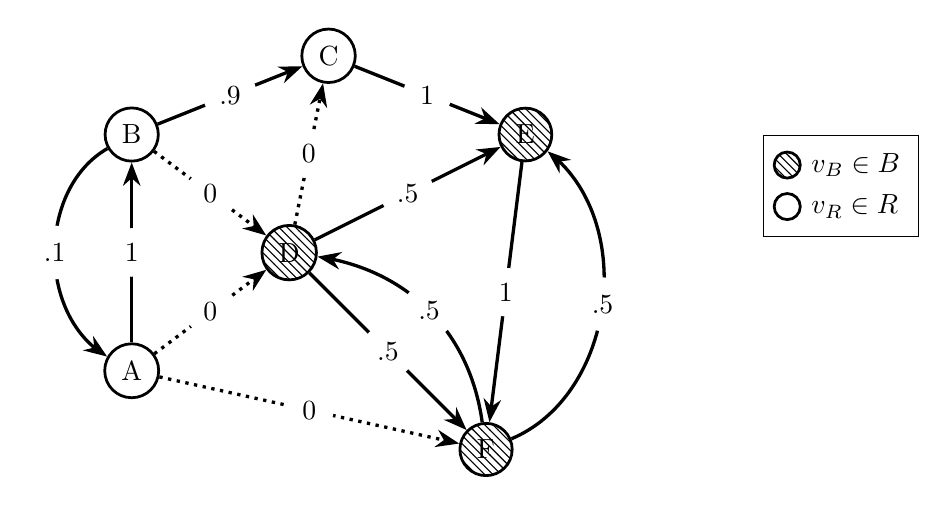
\begin{tikzpicture}
        [
  rednode/.style={shape=circle, draw=black, line width=1},
  bluenode/.style={shape=circle, draw=black, line width=1, pattern=north west lines}
]
        \begin{scope}
            [every node/.style={circle,thick,draw}]
            \node[rednode] (A) at (0,0) {A};
            \node[rednode] (B) at (0,3) {B};
            \node[rednode] (C) at (2.5,4) {C};
            \node[bluenode](D)  at (2,1.5) {D};
            \node[bluenode] (E) at (5,3) {E};
            \node[bluenode] (F) at (4.5,-1) {F} ;
        \end{scope}
        
        \begin{scope}[>={Stealth[black]},
                      every node/.style={fill=white,circle},
                      every edge/.style={draw=black,very thick}]
            \path [->] (A) edge node {$1$} (B);
            \path [->] (B)[bend right=60] edge node {$.1$} (A);
            \path [->] (B) edge node {$.9$} (C);
            \path [->] (A) edge[dotted] node {$0$} (D);
            \path [->] (D) edge[dotted] node {$0$} (C);
            \path [->] (A) edge[dotted] node {$0$} (F);
            \path [->] (D) edge node {$.5$} (F);
            \path [->] (D) edge node {$.5$} (E);
            \path [->] (C) edge node {$1$} (E);
            \path [->] (E) edge node {$1$} (F); 
            \path [->] (B) edge[dotted] node {$0$} (D);
            \path [->] (F)[bend right=60] edge node {$.5$} (E);
            \path [->] (F)[bend right=37] edge node {$.5$} (D);
        \end{scope}

        \begin{scope}
            \matrix [draw,below left] at (10,3){
                \node [bluenode,label=right:$v_B \in B $] {}; \\
                \node [rednode,label=right:$v_R \in R $] {}; \\
              }; 
        \end{scope}
        \end{tikzpicture}
        \caption[]{Esempio di grafo}\label{fig:graph}
    \end{figure}

    Ogni arco $(v_i,v_j)\in E$ ha un peso che indica la probabilità di transizione dal vertice $v_i$ 
    al vertice $v_j$. I pesi degli archi vengono raggruppati in una matrice stocastica-destra $M$ $n\times n$ 
    dove ogni elemento $M(v_i,v_j)$ è una probabilità ($0\le M(v_i,v_j)\le 1$). Se $M(v_i,v_j)=0$ l'arco che collega 
    $v_i$ e $v_j$ non esiste ($(v_i,v_j)\not \in E$). Inoltre, per definizione di matrice stocastica-destra,
    ogni riga di $M$ somma a 1 $(\sum_{v_j=1}^n{M(v_i,v_j)}=1)$.

    \begin{figure}[!h]\label{matrix_graph}
        \[ M =\bordermatrix{ & A & B & C & D & E & F \cr 
                            A &0 &1 &0 &0 &0 &0 \cr
                            B &.1 &0 &.9 &0 &0 &0 \cr
                            C &0 &0 &0 &0 &1 &0  \cr
                            D &0 &0 &0 &0 &.5 &.5 \cr
                            E &0 &0 &0 &0 &0 &1 \cr
                            F &0 &0 &0 &.5 &.5 &0\cr
                            }\]
        \caption{Matrice $M$ per il grafico in \hyperref[fig:graph]{Figura\ \ref{fig:graph}}}
    \end{figure}
    }

    \section{Random walks}
        Un \emph{random walk} è un cammino sul grafo che parte da un vertice $v$ e, ad ogni vertice nel cammino, viene scelto, 
        indipendentemente dalle scelte precedenti, un arco uscente con una probabilità uguale al suo peso. 
        Tornerà utile definire una variabile aleatoria $T_v(S)$ che indica il primo istante di tempo in cui un random walk partito 
        dal vertice $v$ raggiunge un vertice di $S\subseteq V$. Si denota con \emph{``hitting time of $S$ from $v$''} la quantità $\E_G[T_v(S)]$ 
        dove l'aspettazione è calcolata tra tutti i possibili random walk che percorrono $G$ partendo da $v$, con le probabilità di transizione date dalla matrice $M$.
        Nelle realtà, la lunghezza dei random walk è limitata superiormente ad un valore $t$ \emph{(``exploration factor'')}. Questo fattore è ricavato empiricamente: 
        può essere, ad esempio, il numero di pagine web che un utente visita in una sessione web. Per misurare più accuratamente la lunghezza di una sessione web,
        però, si può considerare la variabile aleatoria $T_{v}^{t}(S)=\min\{t,T_v(S)\}$.\\ 
        Dato un grafo $Z$, un qualunque vertice $u$ e un qualunque insieme $S$ di vertici di $Z$, si definisce $u \overset{cond}{\underset{Z}{\leadsto}}S$ 
        l'evento nel quale un random walk percorre $Z$ da $u$ a un vertice di $S$ senza visitare un vertice di $\overline{C}_u$ (di ``colore diverso'') 
        e che soddisfa la condizione $cond$ in termini di step necessari per raggiungere $S$. Ad esempio, $u \overset{=t}{\underset{Z}{\leadsto}}S$ indica l'evento nel quale 
        un random walk su $Z$ partendo da $u$ raggiunge un vertice di $S$ con esattamente $t$ steps, senza visitare vertici di $\overline{C}_u$.

    
    \section{Random-walk closeness centrality}
        Gli algoritmi proposti utilizzano la ``Random-walk closeness centrality'' come discriminante per la scelta dei nuovi archi da aggiungere o per deterimanre gli archi di cui fare ``swapping''.
        Nello specifico, si utilizza la definizione di \emph{Random-walk closeness centrality} per ridurre la lunghezza
        dei random walk nel grafo in modo che il contributo alla centralità di $v$ dei vertici che non raggiungo $v$ in meno di $t'$ steps (in termini di aspettazione) sia uguale a 0, per ogni $t'$.
        \begin{definition}[Closeness centrality]
            La closeness centrality di un vertice è la lunghezza media dei cammini minimi tra un vertice e tutti gli altri vertici del grafo. 
        \end{definition}
        \begin{definition}[Random-walk closeness centrality (bounded)]
            Dato un nodo $v \in V$, un sottoinsieme $S \subseteq V$, il t'-bounded Random Walk Closeness Centrality (RWCC) di $v$ rispetto a $S$ è
            \begin{equation}
                r^{t'}(v;S)\doteq{1\over{|S|}}\sum_{w\in S}\Big(t'-\E_G[T^{t'}_w(v)]\Big)
            \end{equation}
        \end{definition}
        Dato che il calcolo del RWCC esatto è estremamente costoso, verrà utilizzata come stima $\overline{r}(v)$: si prendono $z$ vertici da $S$ (chiamati ${\{w_i\}}_{i=1}^{z}$) 
        ed, eseguendo $k$ random walk, si ottiene la stima $\overline{h}_{w_i}$ di $\E_G[T^{t'}_{w_i}(v)]$ per ogni $w_i$.
        \begin{equation}
            \overline{r}(v)\doteq t' - {1\over{z}}\sum_{i=1}^{z}\overline{h}_{w_i}
        \end{equation}

    \section{Bubble radius}
        Viene introdotto il concetto di \emph{``Bubble Radius''} per quantificare quanti steps, in media, sono necessari affinchè un utente, partendo con un random walk 
        da un vertice $v\in V$ di un dato colore, raggiunga un vertice di un altro colore.
        \begin{definition}[Bubble radius]
            Il Bubble Radius $B_{G}^{t}(v)$ di v con $t$ exploration parameter è
             \begin{equation}
                B_{G}^{t}(v)\doteq \E_G[T_{v}^t(\overline{C}_v)]
            \end{equation}
        \end{definition}
        Data la definizione, è improbabile che un random walk che parte da un vertice $v$, avente un elevato Bubble Radius,
        raggiunga un vertice di colore opposto ($\in\overline{C}_v$) in meno di/esattamente $t$ steps. Per semplicità, 
        si assume di avere l'esatto valore di BR per ogni vertice del grafo.
        \subsubsection*{Estensione a più di 2 colori} 
        Nella trattazione degli algoritmi, si assume l'esistenza di solo 2 colori (Red e Blue). Si può estendere il caso a più colori:
        \begin{itemize}
            \item Dividendo il grafo in 2 ``colori'': il gruppo ``Red'' conterrà tutti i vertici di un dato colore 
            e il gruppo ``Blue'' contenente i vertici aventi tutti gli altri possibili colori.
            \item Assegnando un colore diverso $C_i \, ,1 \le i \le k$, per ogni gruppo di vertici. 
        \end{itemize}
        Nel secondo caso, può essere definito il BR di un vertice $v$ come il minimo tra 
        tutti i $B_G^{t}(v_i) \doteq \E_G[T_{v_i}^t({C}_j)] \; 1 \le j \le k ,j \not = i  $. 



% %\afterpage{\blankpage}

% % Chapter 2
% \clearpage{\pagestyle{plain}\cleardoublepage}
% \chapter{RePBubLik}
% L'idea alla base dell'algoritmo RePBubLik è quella di aggiungere al grafo
della rete sociale archi pesati che permettano di ridurre la polarizzazione 
rispetto ad un dato topic. Di seguito, vengono esposti i principi teorici e 
le metriche per valutare l'efficacia di questo approccio. 

\section{Vertici cosmopolitan e vertici parochial}
In base al valore del Bubble Radius, viene diviso l'insieme dei vertici in 2 
sottoinsiemi: \emph{cosmopolitan} e \emph{parochial}. L'insieme $Z(G)$ dei vertici 
cosmopolitan contiene tutti e soli i vertici di $G$ con un Bubble Radius 
\emph{al più} uguale a $b$ (cioè $\le b$), mentre il l'insieme $P(G)$ dei
vertici parochial contiene tutti e soli i vertici di $G$ con un 
Bubble Radius \emph{almeno} uguale a $r$ (cioè $\ge b$), con $1\le b < r \le t$ 
numeri reali. Importante notare che $Z(G)$ e $P(G)$ sono disgiunti, 
ma non formano necessariamente una partizione di $V$. Nelle analisi, infatti,
partizioneremo il set $P(G)$ a seconda del colore: $P_R(G)$ per i parochial 
aventi colore $R$ e $P_B(G)$ per i parochial aventi colore $B$. 
Questa divisione si basa sulla facilità di un nodo di raggiungere, tramite un random walk, 
un nodo di colore opposto: sarà più facile raggiungere un vertice di colore opposto partendo 
da vertice cosmopolitan e, al contrario, sarà difficile per un vertice parochial.\\
Dato il fatto che i nodi parochial sono i vertici per i quali è più difficile
trovare un random walk che raggiunga un vertice di colore opposto, 
risulta sensato utilizzare i valori dei Bubble Radius di quest'ultimi per stimare la polarizzazione 
(\emph{structural bias}) del grafo.
\begin{definition}[Structural Bias]
    Il Bias Strutturale $\rho(G)$ di $G$ è la somma dei Bubble Radius dei nodi parochial di $G$
    \begin{equation}\label{REP:bias}
        \rho(G)=\sum_{v \in P(G)}{B_{G}^t(v)}
    \end{equation}
\end{definition}
\section{Riduzione del bias strutturale mediante inserimento di archi}
L'obiettivo di RePBubLik sarà quello di cercare un'insieme di archi, aventi come estremi vertici
di colori opposti, da aggiungere al grafo $G$ per diminuire il structural bias. Se, ipoteticamente,
si potesse aggiungere una quantità qualsiasi di archi, chiaramente il bias sarebbe 0, in quanto il 
grafo sarebbe completo. Comprensibilmente, questo non è realistico se si tratta di reti sociali: un browser 
può consentire solo un certo numero di link per pagina e l'essere umano non è in grado di distinguire 
un numero elevato di link all'interno della singola web page.\\
Per queste ragioni, la riduzione del bias strutturale mediante inserimento di archi, diventa un problema
di ottimizzazione.
\begin{definition}
    Dato un set $\Sigma$ di archi non presenti in $G$, si denota con $G_{\Sigma}$ il nuovo grafo $G_{\Sigma}\doteq (V,E \cup \Sigma)$. 
\end{definition}
\begin{problem}\label{problem:1}
    Dato $C \in \{R,B\}$, trovare il più piccolo insieme $\Sigma$ di vertici distinti $(v,w)\not \in E$ con $C_v=C$ e $C_w\not = C$ dove $P_C(G_\Sigma)= \emptyset $.
\end{problem}
In altri termini, il problema da risolvere all'ottimo consiste nel trovare un insieme minimo di archi aventi come estremi vertici di colore opposto, che permetta 
di azzerare il numero di vertici parochial. Il problema \ref{problem:1} è NP-Hard e APX-Hard, cioè un problema non risolvibile all'ottimo in tempo polinomiale,
ma ammette un'approssimazione polinomiale.
\subsection{Approssimazione del problema}
Per approssimare il problema \ref{problem:1}, saranno necessarie delle nuove metriche per analizzare come cambia il grafo $G$
in seguito all'aggiunta di nuovi archi.
\begin{definition}(Guadagno di $U$ grazie a $\Sigma$)
    Si assuma di aggiungere al grafo $G$ tutti gli archi di $\Sigma$, ogni edge  $e=(v,w)$ ha un peso $M(e)$. Per un set $U$ di vertici, si definisce guadagno di $U$ 
    grazie a $\Sigma$
    \begin{equation}\label{REP:gain}
        \Delta(G,U,\Sigma,\{M(e)\}_{e\in\Sigma},t')\doteq {1\over{|U|}}\sum_{u\in U}{\Big(B_{G}^{t'}(u) - B_{G_{\Sigma}}^{t'}(u)\Big)}
    \end{equation} 
\end{definition}
In altri termini, si valuta il cambiamento medio del Bubble Radius dei vertici contenuti in U, cioè quelli coinvolti dagli archi di $\Sigma$.
Ogni arco aggiunto, quindi, deve avere un peso $M(e)$. Questo peso è dato da un oracolo che calcola il peso di un arco $M(v,w)$ in funzione di $v$ e delle informazioni
\emph{locali} di $v$ (es. numero di archi uscenti). Importante notare che, dopo l'aggiunta di un arco $e=(v,w)$, gli altri archi uscenti dal vertice $v$
avranno un peso scalato di $1-M(e)$.
Date queste considerazioni il problema \ref{problem:1} può essere approssimato come segue.
\begin{problem}\label{problem:2}
    Sia $C\in\{R,B\}$. Trovare un set $\Sigma={\{(v_i,w_i)\}}_{i=1}^{k}$ di $k$ archi con $v_i\in C$ e $w_i \not \in C$, per $1\le i \le k$,
    che massimizzi $\Delta(G,P_C(G),\Sigma,\{M(e)\}_{e\in\Sigma},t)$.
\end{problem}
RePBubLik è l'algoritmo che approssima il problema \ref{problem:2}.
\begin{definition}
    Per un qualsiasi vertice $v$ e $ 0 \le t' \le t $, sia
    \begin{equation}\label{eq:F}
        F_{t'}(v)\doteq 1 -\Prob\Big( v \overset{<t'}{\underset{G}{\leadsto}}v\Big)
    \end{equation}
\end{definition} 
Questa quantità è uno (cioè la probabilità di avere un random walk da $v$ che torni a $v$ in 0 passi) più la probabilità che un random walk da $v$ finisca in $v$
in meno di $t'$ steps.
\begin{theorem}[Approssimazione di RePBubLik]
    Sia $\Sigma$ l'output di RePBubLik e $OPT$ la soluzione ottima al problema \ref{problem:2}. 
    Sia $\Delta_{\Sigma}=\Delta(G,P_C(G),\Sigma,\{M(e)\}_{e\in\Sigma},t)$. Allora
    \begin{equation}
        \Delta(G,P_C(G),OPT,\{M(e)\}_{e\in OPT},t) \le \Big(2{t\over{r}}\gamma_{t-2} + 1\Big)\Big(1+{1\over{e}}\Big)\Delta_{\Sigma}
    \end{equation}
    dove $\gamma_t\doteq \max_{v\in V} F_{t'}(v)$
\end{theorem}
Dunque, RePBubLik fornisce una \emph{approssimazione a fattore costante}, sotto l'assunzione che $\gamma_t$ sia una costante e che $r\ge t/2$.
\section{RePBubLik: definizione intuitiva}
Dato il fatto che la funzione obiettivo (guadagno $\Delta$) è \emph{monotona} e \emph{sub-modulare}, la scelta gli archi da aggiungere al grafo $G$ può essere efftuata in maniera greedy.
L'assunzione sui pesi che l'oracolo assegna agli archi, inoltre, garantisce che \emph{ogni} vertice di colore diverso da quello di partenza può essere scelto come estremo dell'arco, 
senza che il peso di quest'ultimo venga modificato. Con queste assunzioni, si semplifica notevolmente il calcolo: invece che cercare le coppie $(v,w)$ da aggiungere a $G$, sarà necessario cercare solamente 
solamente i \emph{vertici di partenza} da cui escono i nuovi archi. \\
Per la scelta greedy, un buon candidato $v$ è il vertice che con maggior probabilità viene raggiunto da molti altri vertici in $P_{C_v}(G)$, attraverso random walk brevi. 
Questa proprietà è espressa dal bounded RWCC $r^{t-2}(v,P_{C_v}(G))$.
\newpage
\section{RePBubLik: pseudocodice}
\begin{algorithm}[!h]
    \caption{RePBubLik}\label{alg:repbublik}
    \begin{algorithmic}
    \Require Grafo $G=(V,E)$, numero $k$ di archi che vogliamo inserire, oracolo $W_G: V \times 2^{V\times V} \to [0,1]$, $C\in\{R,B\}$
    \Ensure L'insieme $\Sigma$ di $k$ archi da aggiungere, con relativi pesi.
    \\
    \State $\Sigma \gets \emptyset$
    \For{$i=1 ,\dots, k$}
        \State $P \gets computeParochials(G_{\Sigma},C)$
        \State $R \gets computeRWCentrality(P,G_{\Sigma})$
        \State $v_i \gets \arg\max_{v \in P} R(v)\times W_G(v,\Sigma)$
        \State $u_i \gets arbitrary \; in \; \overline{C}_{v_i}$
        \State $\Sigma \gets \Sigma \cup \{(v_i,u_i)\}$
    \EndFor
    \State\Return $\Sigma$
    \end{algorithmic}
\end{algorithm}
L'algoritmo RePBubLik prende come input un grafo $G$, un numero $k$ di archi da inserire, 
un oracolo $W$ che fornisce il peso dei nuovi archi e un set $C\in\{R,B\}$ di nodi di un dato colore.\\
Per prima cosa, viene creato l'insieme $\Sigma$ (inizialmente vuoto) che conterrà gli archi da aggiungere.
Successivamente, per $k$ volte: viene calcolato il Bubble Radius di ogni nodo in $C$ nel grafo $G_\Sigma$, ottenuto 
aggiungendo a $G$ gli archi contenuti in $\Sigma$. Si ottiene, così, un set $P$ di nodi parochial del grafo $G_\Sigma$.
In seguito, si calcola il RWCC $r^{t-2}(v,P)$ di ogni nodo $v\in P$ e questi valori vengo salvati in un dizionario $R$.
Una volta popolato $R$, viene scelto il nodo $v_i\in P$ avente il valore più alto di $R(v_i)\times W_G(v_i,\Sigma)$ e un 
qualsiasi nodo $u_i$ di colore $\overline{C}_{v_i}$. Così facendo, si ottiene l' arco $(v_i,u_i)$ da aggiungere all'insieme $\Sigma$.
Dopo le $k$ iterazioni, infatti, l'insieme $\Sigma$ sarà popolato da $k$ archi, il cui peso è deciso dall'oracolo.
\subsection{RePBubLik+}
Come si può notare dallo pseudocodice, RePBubLik ripete il calcolo del Bubble Radius di \emph{tutti i vertici}  e del RWCC di \emph{tutti i vertici in $P$} 
ad \emph{ogni iterazioni} del ciclo. Questo, a livello computazionale, è molto oneroso.\\
Dunque, una pratica alternativa a RePBubLik è una sua versione approssimata (RePBubLik+) che calcola il Bubble Radius e RWCC una \emph{sola
volta, prima di entare nel ciclo}. Chiaramente, questa approssimazione non permette di ottenere garanzie rigorose sull'approssimazione calcolata, 
ma diventa necessaria per diminuire il tempo di esecuzione dell'algoritmo.



    


% %\afterpage{\blankpage}

% % Chapter 3
% \clearpage{\pagestyle{plain}\cleardoublepage}
% \chapter{ShuffLik}
% L’idea alla base dell’algoritmo ShuffLik è quella di scambiare i pesi degli archi aventi lo stesso vertice di partenza, per 
aumentare la navigabilità della rete. 
Di seguito, vengono esposti i principi teorici e 
le metriche per valutare l'efficacia di questo approccio. 

\section{Diverse navigability}
In molte reti sociali, l'aggiunta di archi è spesso un'operazione invasiva e non sempre possibile. 
Se si pensa, ad esempio, ai sistemi di raccomandazione (es. articoli suggeriti di Amazon) risulta evidente il fatto che il numero di elementi 
consigliabili è limitato. Per questo motivo, l'approccio di RePBubLik è inefficiente e quindi si dovrà considerare una nuova 
misura che chiameremo \emph{diverse navigability} che tiene in considerazione i valori di Bubble Radius di \emph{tutti} i vertici della rete.
\begin{definition}[Diverse navigability]
    Dato $S \subseteq V$, la diverse navigability $\xi(S)$ di $S$ è l'opposto del Bubble Radius medio dei vertici in $S$.
    \begin{equation}
        \xi(S)\doteq - {1\over{|S|}}\sum_{v\in S}{B_{G}^t(v)}
    \end{equation}
    Quando $S=V$, si parla di diverse navigability del grafo $G$; si denota con $\xi(G)$
\end{definition}

\section{Aumento della navigabilità mediante lo scambio delle probabilità di transizione}
L'idea alla base di ShuffLik è quella di aumentare la navigabilità di una rete scambiando tra loro i pesi 
di due archi appartenenti allo stesso vertice (es. pagina web).
Questo nella pratica è molto sensato: numerosi studi hanno dimostrato che la probabilità che un certo link venga cliccato è spesso collegata da fattori grafici 
quali posizione, colore o font. Scambiare, quindi, la posizione dei link all'interno della pagina permetterebbe alla rete di essere più fruibile e navigabile.
Per questo, si definisce l'insieme dei \emph{diversifying swaps} come l'insieme delle coppie di archi che risultano ragionevoli da scambiare, per aumentare 
la diverse navigability.
\begin{definition}[Diversifying swaps]
    Per $C \in \{R,B\}$, l'insieme $D_C$ dei diversifying swaps è l'insieme di coppie ordinate di archi, dove per ogni $(e,e')$ vale che:
    \begin{enumerate}
        \item $(e,e')=((v,w),(v,u))$ con $v,w \in C$ e $u \in \overline{C}_v$
        \item $M(e) > M(e')$
    \end{enumerate} 
\end{definition}
Sostituire il peso di $e$ con il peso $e'$ della coppia $(e,e') \in D_C$, permette di diminuire il Bubble Radius del vertice di partenza $v$ ,
aumentando così la diverse navigability $\xi(C_v)$ e, conseguentemente, la $\xi(G)$.
\\
Per quantificare il miglioramento apportato da questo swap, sarà necessaria una qualche misura di guadagno.
\begin{definition}[Guadagno sul BR di $u$ dato dallo swap di $e$ con $e'$]
    Per $C \in \{R,B\}, u\in C$ e $t' \le t$, il guadagno $\Gamma(G,u,(e,e'),t')$ sul Bubble Radius di $u$
    ottenuto dallo swap della probabilità di transizione di $(e,e')\in D_C$, è definito come
    \begin{equation}\label{SHU:gain}
        \Gamma(G,u,(e,e'),t')\doteq B_{G}^{t'}(u) - B_{G_{e,e'}}^{t'}(u)
    \end{equation}
    dove $G_{e,e'}$ è il grafo $G$ dopo aver scambiato i pesi tra $e$ ed $e'$.
\end{definition}
Chiaramente, il guadagno totale può essere ottenuto estendendo la definizione \ref{SHU:gain} all'intero \emph{diversifying swaps}.
\begin{definition}[Guadagno totale]
    Sia $\Sigma \subseteq D_{C}$ e $G_{\Sigma}$ il grafo ottenuto scambiando tra loro tutti i pesi delle coppie contenute 
    in $\Sigma$. Il guadagno totale di $\Sigma$ è definito
    \begin{equation}
        \mathbb{G}(G,\Sigma)\doteq {1\over{|C|}}\sum_{u\in C}{\Big(B_{G}^{t}(u) - B_{G_{\Sigma}}^{t}(u) \Big)}
    \end{equation}
\end{definition}
\subsection{Approssimazione del problema}
Risulta evidente che scambiare tra loro tutti gli archi contenuti in $D_C$ diventa un operazione onerosa e non ragionevole nella pratica.
Per questo, si assume che il numero di possibili swaps sia limitato ad un numero $k$.
\begin{problem}\label{problem:3}
    Dato un grafo $G$, un colore $C$, e un parametro $k$, trovare un set $\Sigma \subseteq D_C$ di dimensione $k$ che 
    massimizzi il guadagno $\mathbb{G}{(G,\Sigma)}$. 
\end{problem}
ShuffLik è l'algoritmo che approssima la soluzione del problema \ref{problem:3}.
\begin{theorem}[Approssimazione di ShuffLik]
    Sia $\Sigma \subseteq D_C$ l'output di ShuffLik e OPT la soluzione ottima al problema \ref{problem:3}. Allora
    \begin{equation}
        \mathbb{G}(G,OPT) \le \Bigg(2{t\over{r}}\gamma_{t-2}+1\Bigg)\Bigg(1+{1\over{e}}\Bigg)\mathbb{G}(G,\Sigma)
    \end{equation}
    dove $\gamma_t\doteq \max_{v\in V} F_{t'}(v)$ (\ref{eq:F})
\end{theorem}
Dunque, ShuffLik fornisce una \emph{approssimazione a fattore costante}, sotto l'assunzione che $\gamma_t$ 
sia una costante e che $r \ge t/2$
\section{ShuffLik: definizione intuitiva}
Dato il fatto che la funzione obiettivo (guadagno $\mathbb{G}$) è \emph{monotona} e \emph{sub-modulare}, la scelta
della coppia di archi da scambiare può essere effetuata in maniera greedy. La scelta greedy deve considerare la coppia $(e,e')$ che massimizza il guadagno.
Ma questa operazione non è per niente banale.\\ 
Verrà selezionata, quindi, la coppia $(e,e')$ che \emph{approssima} la scelta greedy.
Per far ciò, ShuffLik prediligerà la coppia $(e,e') \in D_C$, con vertice iniziale $v$, che massimizza 
la quantità $r^{t-2}(v,C)\times |M(e)-M(e')|$, dove $r^{t-2}(v,C)$ è il RWCC di $v$.
\section{ShuffLik: pseudocodice}
\begin{algorithm}[!h]
    \caption{ShuffLik}\label{alg:shufflik}
    \begin{algorithmic}
    \Require Grafo $G=(V,E)$, matrice di transizione $M_G$, colore $C \in \{R,B\}$, numero di swaps desiderati $k$.
    \Ensure L'insieme $\Sigma$ di $k$ coppie di archi che devono essere scambiati.
    \\
    \State $\Sigma \gets \emptyset$
    \For{$i=1 ,\dots, k$}
        \State $D_C \gets getDiversifyingSwaps(G,C,\Sigma)$
        \State $R \gets computeRWCentrality(C)$
        \State $(e,e') \gets \arg\max_{(e,e') \in D_C} R(v)\times (M_G(e)-M_G(e'))$
        \State $\Sigma \gets \Sigma \cup \{(e_i,e'_i)\}$
    \EndFor
    \State\Return $\Sigma$
    \end{algorithmic}
\end{algorithm}
L'algoritmo ShuffLik prende come input un grafo $G$, la matrice di transizione $M_G$, 
il numero $k$ di swap desiderati e un insieme di nodi di colore $C$. \\
Per prima cosa, viene creato l'insieme $\Sigma$ (inizialmente vuoto) che conterrà le coppie 
di archi da scambiare. Successivamente, per $k$ volte: si ottiene 
l'insieme diversifying swaps $D_C$, utilizzando la funzione \emph{getDiversifyingSwaps}.
Quest'ultima prende come parametri il grafo $G$, il colore $C$, l'insieme $\Sigma$ e ritorna il set
$D_C$ dei possibili swap del grafo $G_\Sigma$, ottenuto scambiando i pesi degli archi in $\Sigma$. 
Per determinare l'insieme $D_C$, la subroutine dovrà valutare Bubble Radius di tutti i vertici in $C$.
In seguito, si calcola il RWCC di ogni nodo in $C$, il quale viene salvato in un dizionario $R$. 
A questo punto, ShuffLik selezione la coppia $(e,e')$ associata al valore più alto di $R(v)\times |M_G(e)-M_G(e')|$,
con $v$ il vertice sorgente di $(e,e')$. Così facendo, si ottiene la coppia di archi $(e,e')$ da aggiungere all'insieme $\Sigma$.
Dopo le $k$ iterazioni, infatti, l'insieme $\Sigma$ sarà popolato da $k$ coppie di archi da scambiare.
\subsection{ShuffLik+}
L'algoritmo ShuffLik presuppone che lo scambio dei pesi abbia un costo fisso. 
Più generalmente, nel caso in cui il costo per effettuare lo swap tra i pesi di due archi non sia un valore fisso e ci sia un budget di costo
da rispettare, si utilizza un approccio simile a ShuffLik, ma con un funzione di costo $Q: E\times E \to \mathbb{R}$ e un budget $B \in \mathbb{R}^+$ da 
non superare. Questa versione modificata dell'algoritmo ShuffLik prende il nome di ShuffLik+.



% %\afterpage{\blankpage}

% % Chapter 4
% \clearpage{\pagestyle{plain}\cleardoublepage}
% \chapter{Valutazione Sperimentale}
% In questa capitolo verranno valutate le performance dell'algoritmo RePBubLik+, confrontadolo
con altri due algoritmi noti per la riduzione della polarizzazione dei grafi: ROV e Node2Vec.

\section{Algoritmi confrontati}
\subsection{ROV(Recommend Opposing View)}
L'algoritmo ROV\cite{ROV} fornisce come output un insieme di $k$ archi da aggiungere a $G$ per minimizzare
il controversy score (Random Walk Controversy). Questa è una metrica che caratterizza quanto un topic
è ``controverso'', cioè quanto è ben separato rispetto agli altri topic. L'algoritmo ROV prende come 
archi candidati quelli che collegano i vertici ad alto grado (con molti archi incidenti) di ciascun "colore"
(topic). Gli archi vengono ordinati in ordine decrescente in funzione del loro impatto sul RWC nel grafo, 
e di questi si individuano i migliori $k$ da aggiungere al grafo G.

\subsection{Node2Vec}
L'algoritmo Node2Vec\cite{Node2Vec} permette di rappresentare un grafo in uno spazio vettoriale a bassa dimensionalità, mantenendo
inalterate alcune caratteristiche importanti della rete come, ad esempio, la similiarità tra nodi.
La generazione di questo spazio vettoriale si basa sui random walk del grafo. Sullo spazio generato,
vengono generalmente eseguiti e addestrati algoritmi di raccomandazione di link. Questo processo permette
di migliorare il suggerimento di nuovi collegamenti all'interno del grafo.
\\
Nell' esperimento svolto, per ogni grafo, viene generato uno spazio a 128 dimensioni e, su quest'ultimo, verrà addestrato
un algoritmo di regressione logistica. Successivamente, verrà predetta la probabilità di esistenza di ciascun arco uscente da $P(G)$.
Al termine, verranno scelti i migliori $k$ archi da aggiungere al grafo $G$, in funzione della loro probabilità.

\section{Dataset}
Nelle analisi, vengono generati grafi dai dataset di \href{https://snap.stanford.edu/data/amazon-meta.html}{Amazon} e \href{http://www-personal.umich.edu/~mejn/netdata/}{PolBlogs}.
%Tabella riassuntiva caratteristiche
\begin{itemize}
\item Il dataset di Amazon contiene informazioni sui libri venduti. Ogni libro è un vertice e 
appartiene ad una categoria (ad un ``colore''). Esiste un arco diretto $(u,v)$ nel grafo se $v$ appartiene alla lista di 
libri simili a $u$ e il suo peso è determinato dal ``sales rank'' di $v$. Da questo dataset, si ottengono tre grafi formati
dalle seguenti coppie di categorie: \emph{Mathematics - Technology}(MaTe), \emph{History of Technology - Military Science}(MiHi) e
\emph{Mathematics - Astronomy }(MaAs).  
\item Il dataset di PolBlogs è una rete diretta di link tra weblogs sulla politica americana. Ogni nodo rappresenta un blog ed è 
``colorato'' in funzione del suo orientamento politico. I link tra i blogs (gli archi nel nostro grafo) sono estratti automaticamente 
da una scansione della pagina principale dei blog. Il peso di un arco $(v,u)$ è dato dal numero di archi uscenti dal vertice $v$.
\end{itemize}
Di seguito una tabella riassuntiva delle statistiche dei grafi generati.
\begin{table}[!h]
    \centering
    \begin{tabular}{lcccccccc}
        \hline
        \multicolumn{9}{c}{\emph{Amazon}} \\
        Topic    & $|V|$ &  $|R|$ & $|B|$ & $|E|$ &  $|E|_{R \to B}$ & $|E|_{B \to R}$ & $\%P_R(G)$ & $\%P_B(G)$\\
        \hline
        \emph{MaTe} & 1393 & 827 & 566 & 675 & 25 & 42 &  90.91 & 79.63\\
        \emph{MiHi} & 851 & 446 & 405 & 482 & 66 & 63 &  58.33 & 63.46\\
        \emph{MaAs} & 1121 &827 & 294 & 680 & 11 & 6 &  97.31 & 95.15\\
        \hline
        \multicolumn{9}{c}{\emph{PolBlogs}} \\
        Topic    & $|V|$ & $|R|$ & $|B|$ & $|E|$ & $|E|_{R \to B}$ & $|E|_{B \to R}$ & $\%P_R(G)$ & $\%P_B(G)$\\
        \hline
        \emph{PolBlogs} & 1033 & 545 & 488 & 17348 & 902 & 781 &  87.71 & 90.37\\
        \hline
    \end{tabular}
    \caption{Tabella delle statisiche dei grafi.
    La colonna $|V|$ specifica il numero di vertici appartenenti al grafo corrispondente.
    Le colonne $|R|$ e $|B|$ indicano, rispettivamente, il numero di vertici di colore $R$ e $B$. 
    La colonna $|E|$ indica il numero di archi del grafo corrispondente.
    Le colonne $|E|_{B \to R}$ e $|E|_{R \to B}$ specificano, rispettivamente, il numero di archi che vanno da nodi di colore $R$ a $B$ e  il numero di archi che vanno da nodi di colore $B$ a $R$.
    Le colonne $\%P_{R}(G)$ e $\%P_{R}(G)$ specificano la percentuale di nodi parochial del grafo $G$ rispettivamente di colore $R$ e $B$.}
\end{table} 
\section{Parametri dei test}
Per ogni grafo, sono stati eseguiti gli algoritmi RePBubLik+, ROV e Node2Vec, con valori crescenti
di $K$ (numero di archi da aggiungere) e con valori di $t$, ovvero la lunghezza massima dei random walk. 
Il valore massimo di $K$ è stato assegnato a 400, per tutti e quattro i grafi in esame.
Da notare che, per come è stato ideato lo script degli algoritmi, il numero finale di archi aggiunti
può essere ben inferiore al numero $K$ impostato manualmente. Per ogni grafo, infatti, vengono allocati $k_B$ archi per il colore $B$ e $k_R$ archi 
per il colore $R$, in proporzione alla somma dei Bubble Radius dei vertici parochial di ciascun colore.
Questo metrica permette di aggiungere più archi per il colore avente più vertici parochial.
Nei grafi in esame, verranno assegnati circa 200 archi per ogni colore.
\\
Per ciascuna esecuzione, verranno analizzati: i tempi d'esecuzione degli algoritmi, il guadagno $\Delta(G,\Sigma)$(\ref{REP:gain}) e il bias strutturale $\rho(G)$(\ref{REP:bias}).
%\newpage
\section{Risultati}
\subsection{Tempi di esecuzione}
Per valutare l'efficacia in termini di tempo degli algoritmi proposti, sono stati eseguiti 10 test per ciascun grafo e per ciacun valore di $t$.
Durante i test, son stati misurati i tempi impiegati dalle varie procedure per determinare i possibili archi candidati. 
Di questi 10 valori, è stata calcolata la media, ottenendo così una stima qualitativa.
Di seguito i grafici riassuntivi dei tempi d'esecuzione.\footnote{Per come è stato ideato lo scpript dagli autori, il tempo totale d'esecuzione comprende alcune varianti di RePBubLik+ 
che non sono oggetto delle analisi effetuate. Considerando l'esecuzione di queste varianti come un fattore costante, il tempo totale 
fornisce una stima approssimativa del tempo totale d'esecuzione.}
\begin{figure}[!h]
    \centering
\begin{subfigure}[h]{0.55\columnwidth}
    \centering
    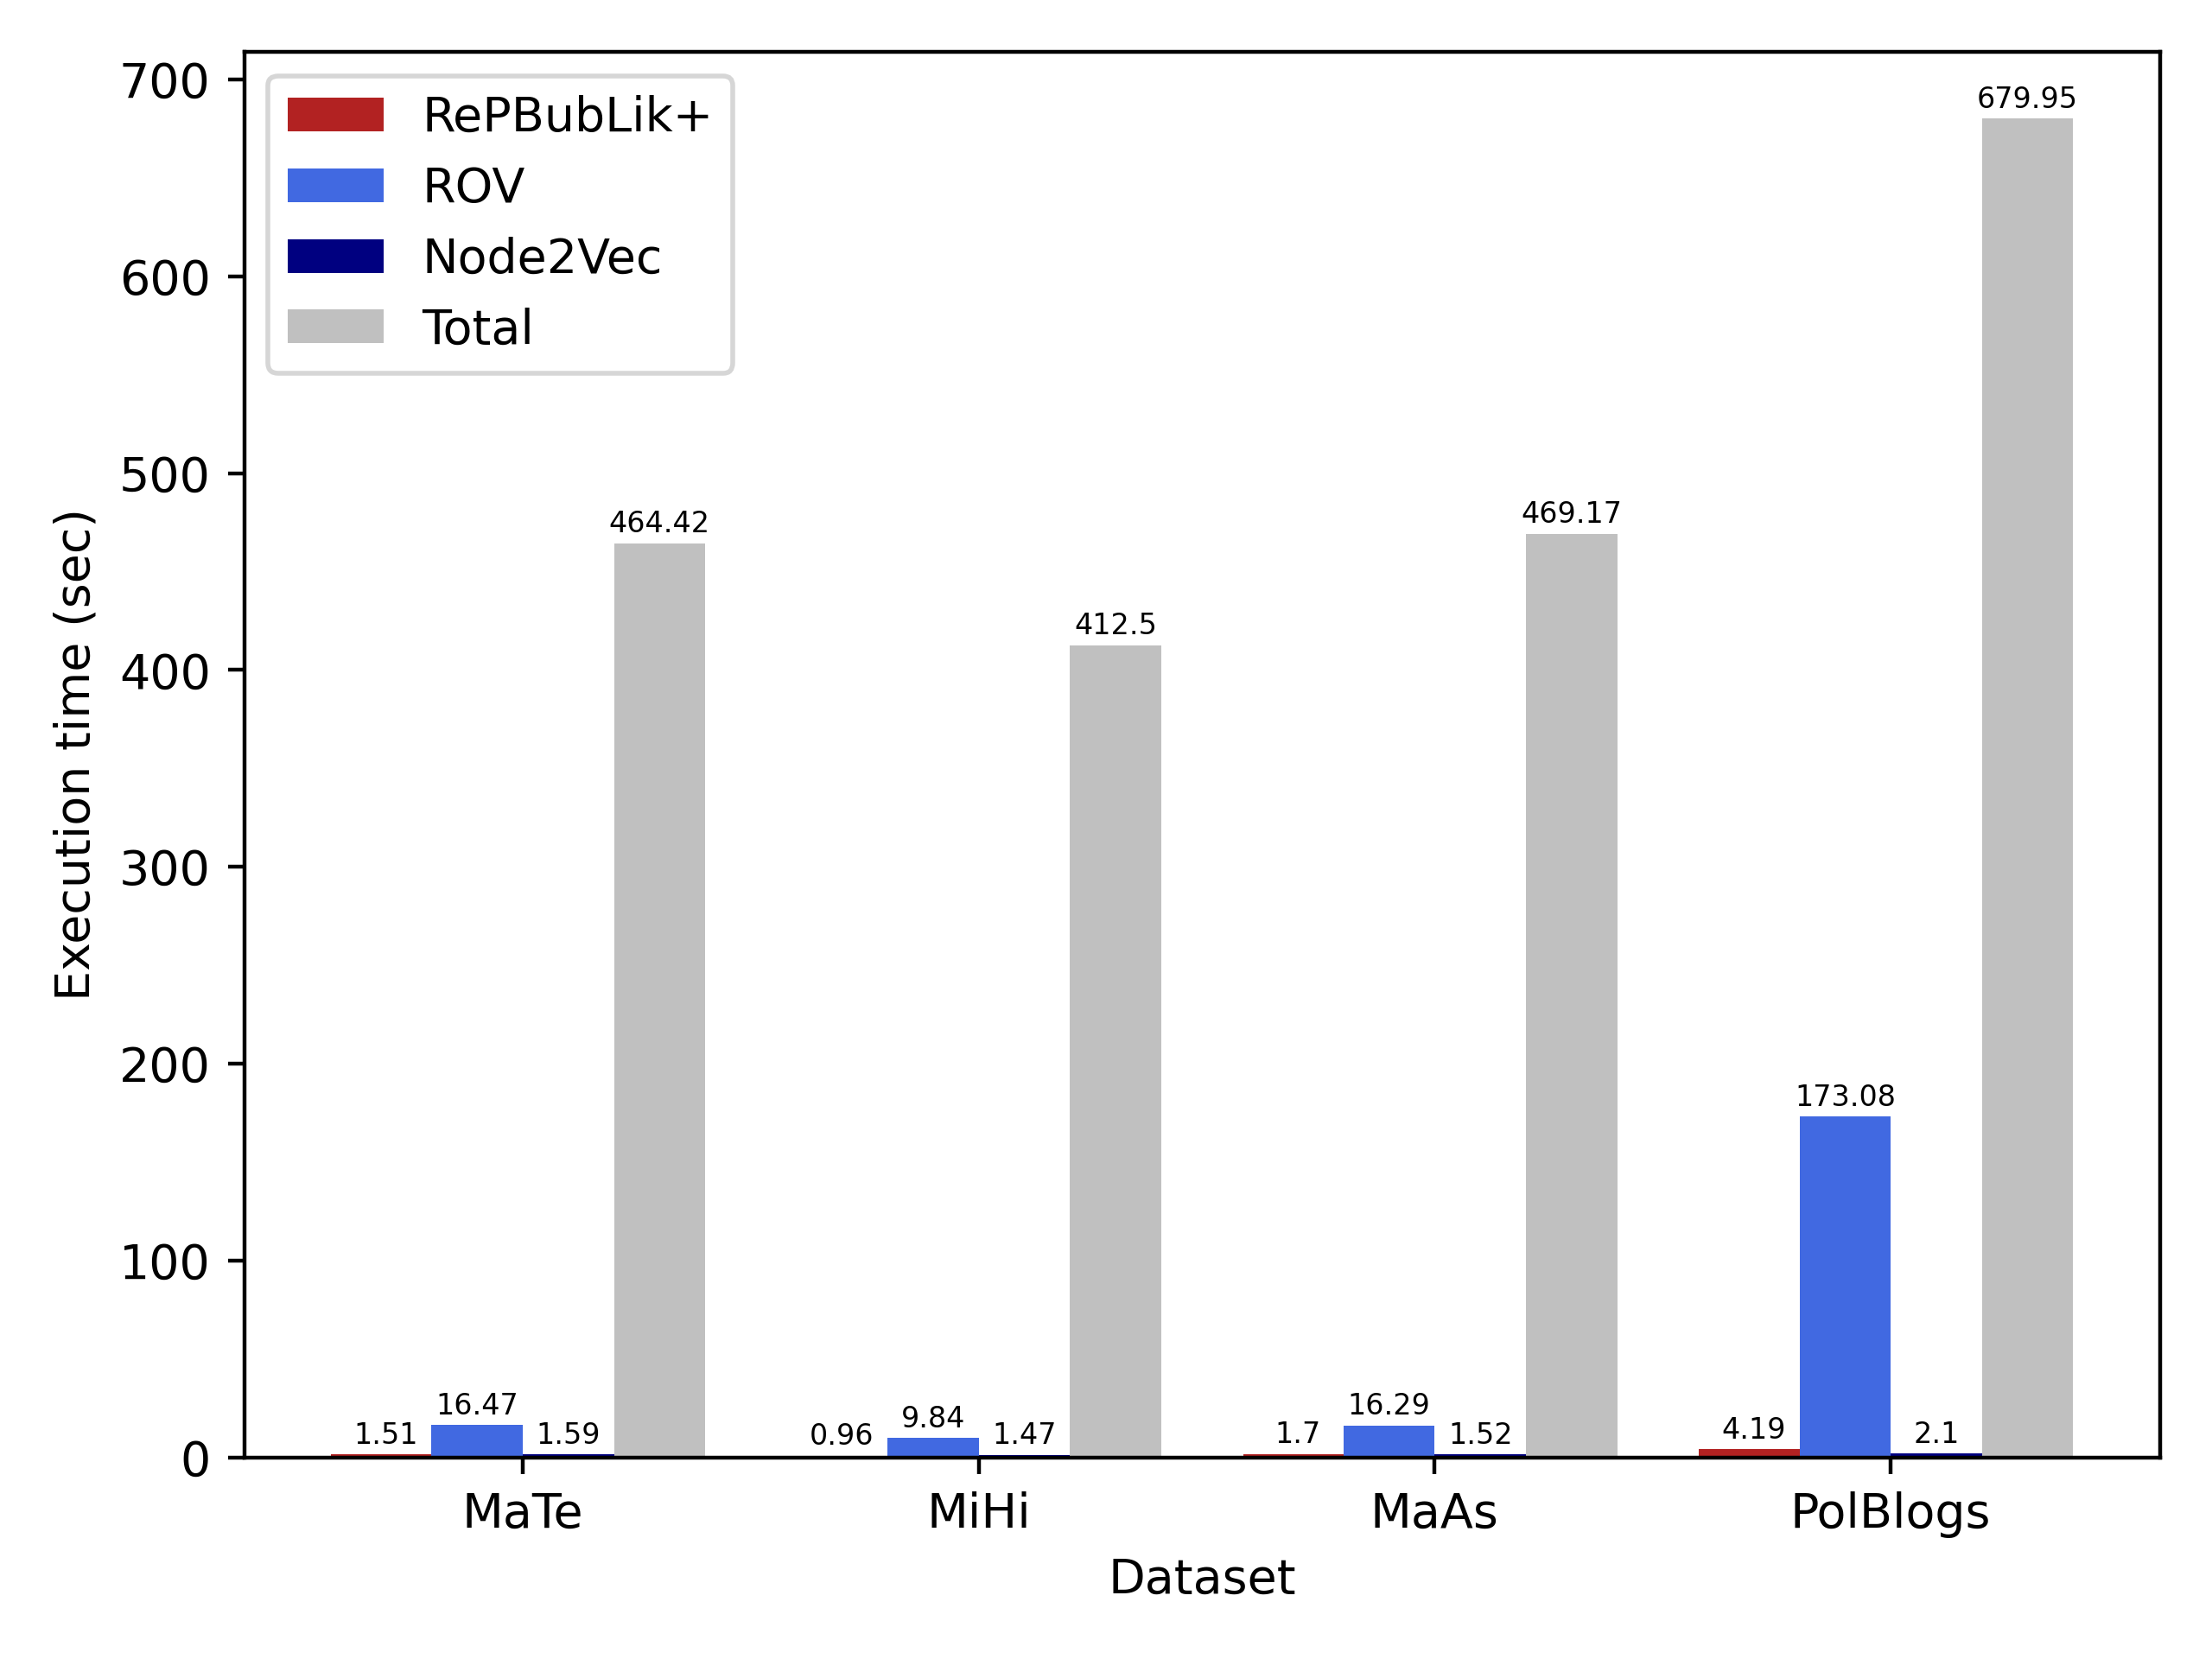
\includegraphics[width=\columnwidth]{5/ex_time_5.png}
    \caption{Parametro $t=5$}\label{fig:mate_e_5}
\end{subfigure}
\begin{subfigure}[h]{0.55\columnwidth}
    \centering
    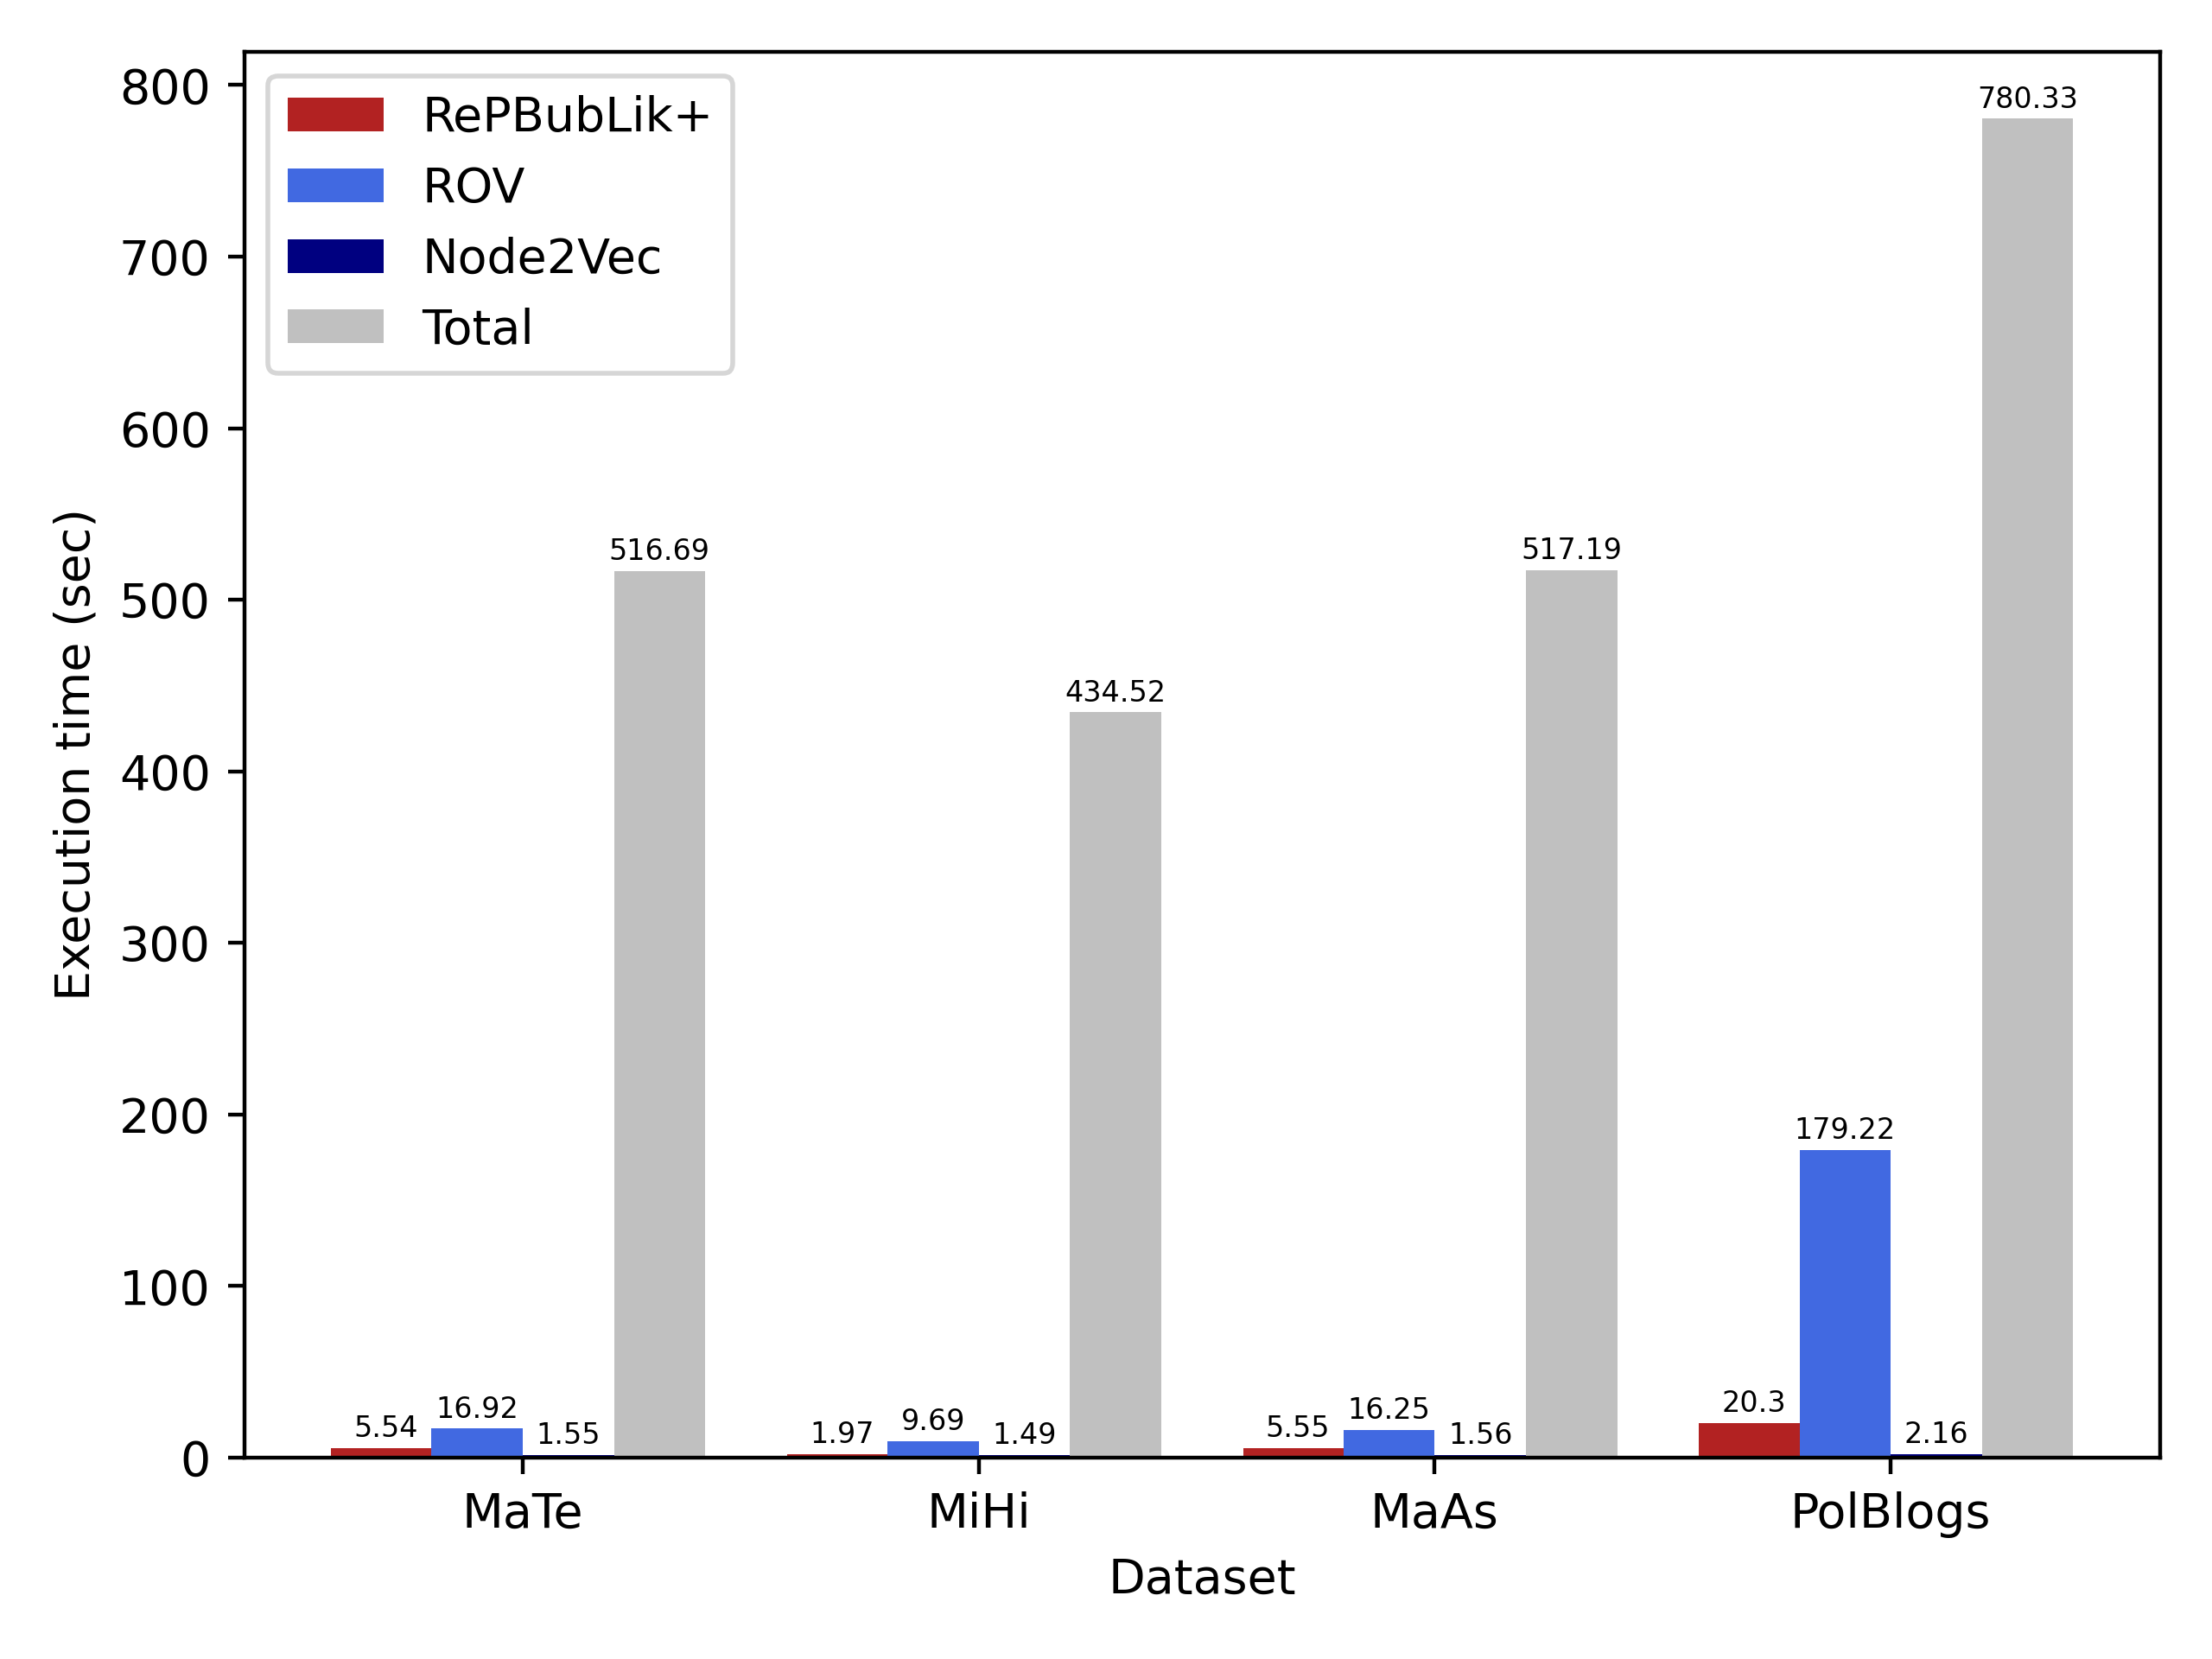
\includegraphics[width=\columnwidth]{10/ex_time_10.png}
    \caption{Parametro $t=10$}\label{fig:mihi_e_10}
\end{subfigure}
   
\end{figure}
\begin{figure}
\ContinuedFloat
\centering
\begin{subfigure}[h]{0.55\columnwidth}
    \centering
    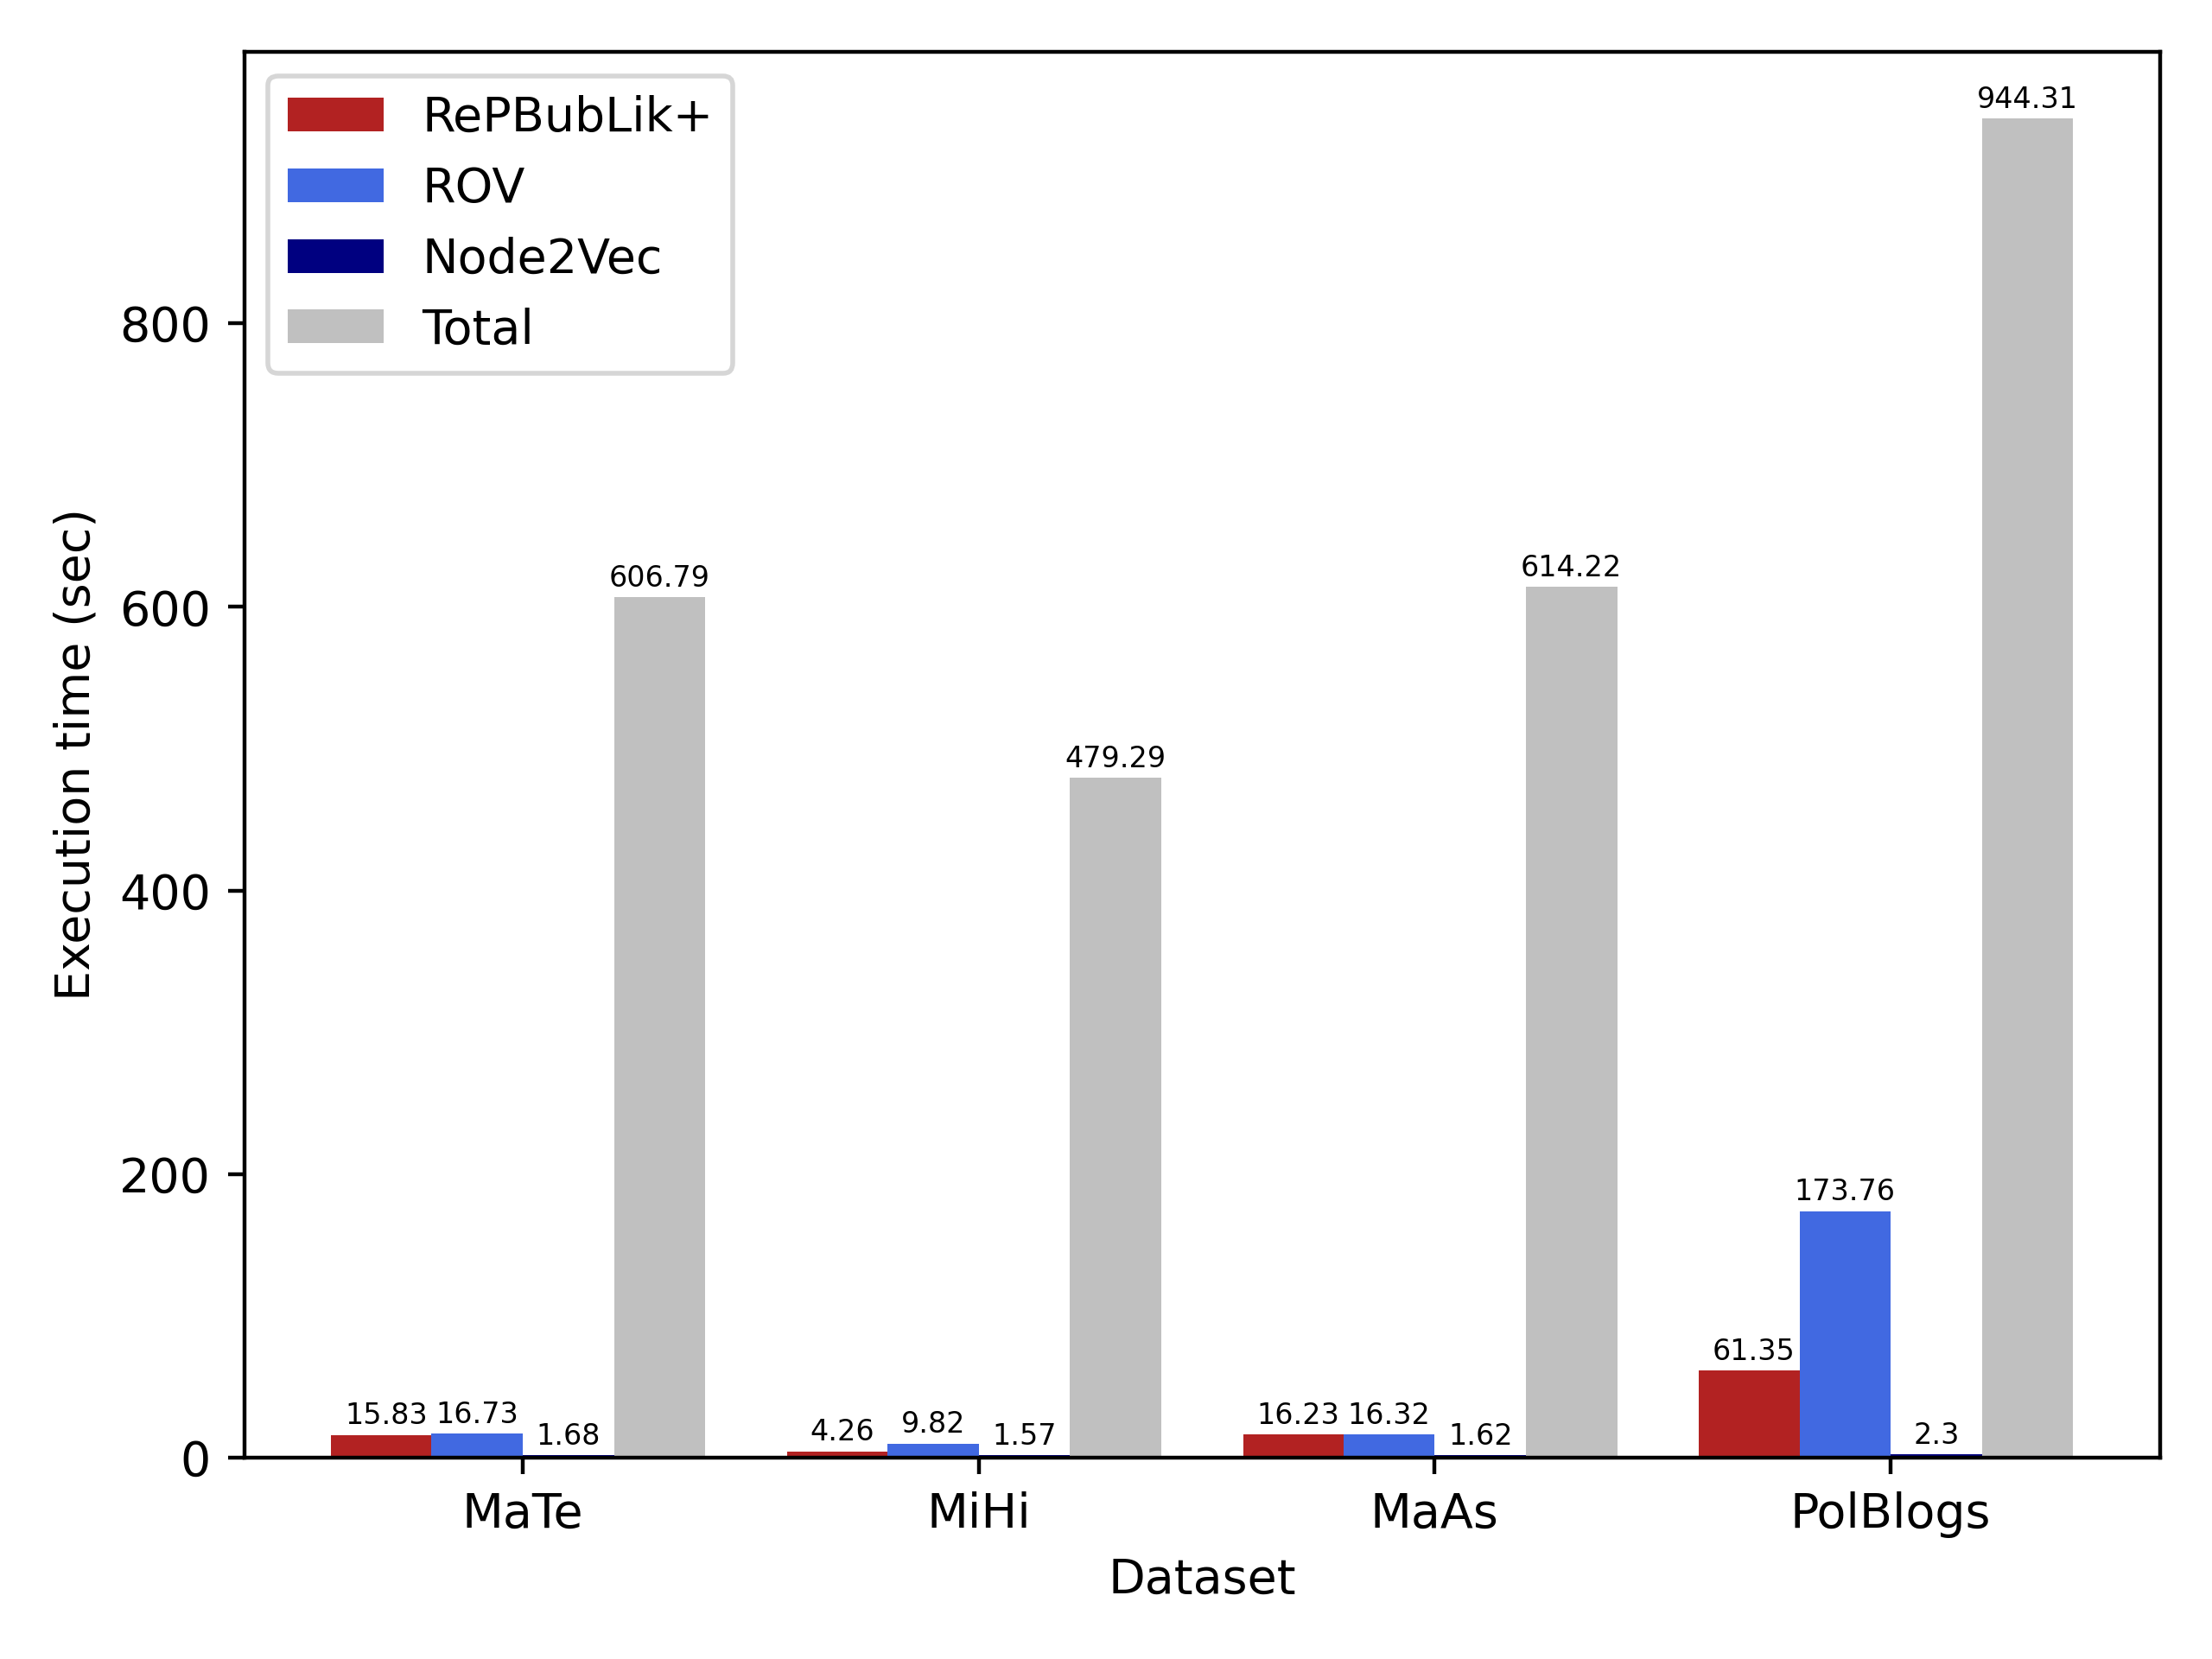
\includegraphics[width=\columnwidth]{15/ex_time_15.png}
    \caption{Parametro $t=15$}\label{fig:maas_e_15}
\end{subfigure}
\caption{Grafici dei tempi d'esecuzione}
\end{figure}
\newpage
Analizzando i grafici dei tempi di esecuzione, si possono trarre le seguenti conclusioni:
\begin{enumerate}
    \item Il tempo impiegato da ciascuna procedura aumenta in relazione alle dimensioni del grafo su cui è applicata.
    \item Node2Vec risulta essere il migliore in termini di tempo d'esecuzione, per ogni grafo e per ogni valore di $t$.
    \item Per ciascun grafo, l'esecuzione di ROV impiega all'incirca lo stesso tempo, indipendentemente dal valore di $t$. 
            Questo è dato dal fatto che ROV utilizza delle metriche differenti dagli altri algoritmi proposti.
    \item RePBubLik+ ha tempistiche intermedie tra quelle di ROV e Node2Vec.
\end{enumerate}
\subsection{Guadagno $\Delta(G,\Sigma)$}
La seconda metrica che viene anlizzata è il il guadagno $\Delta(G,\Sigma)$ (\ref{REP:gain}) in relazione al numero 
degli archi aggiunti al grafo $G$. Lo studio di questa misura è interessante, in quanto permette di valutare il cambiamento medio del Bubble Radius dei vertici parochial $P(G)$.
\\
Nella pagina successiva, i guadagni per ciascun grafo e per ciascun valore di $t$.
\begin{figure}[!h]
    \centering
\begin{subfigure}[h]{0.4\textwidth}
    \centering
    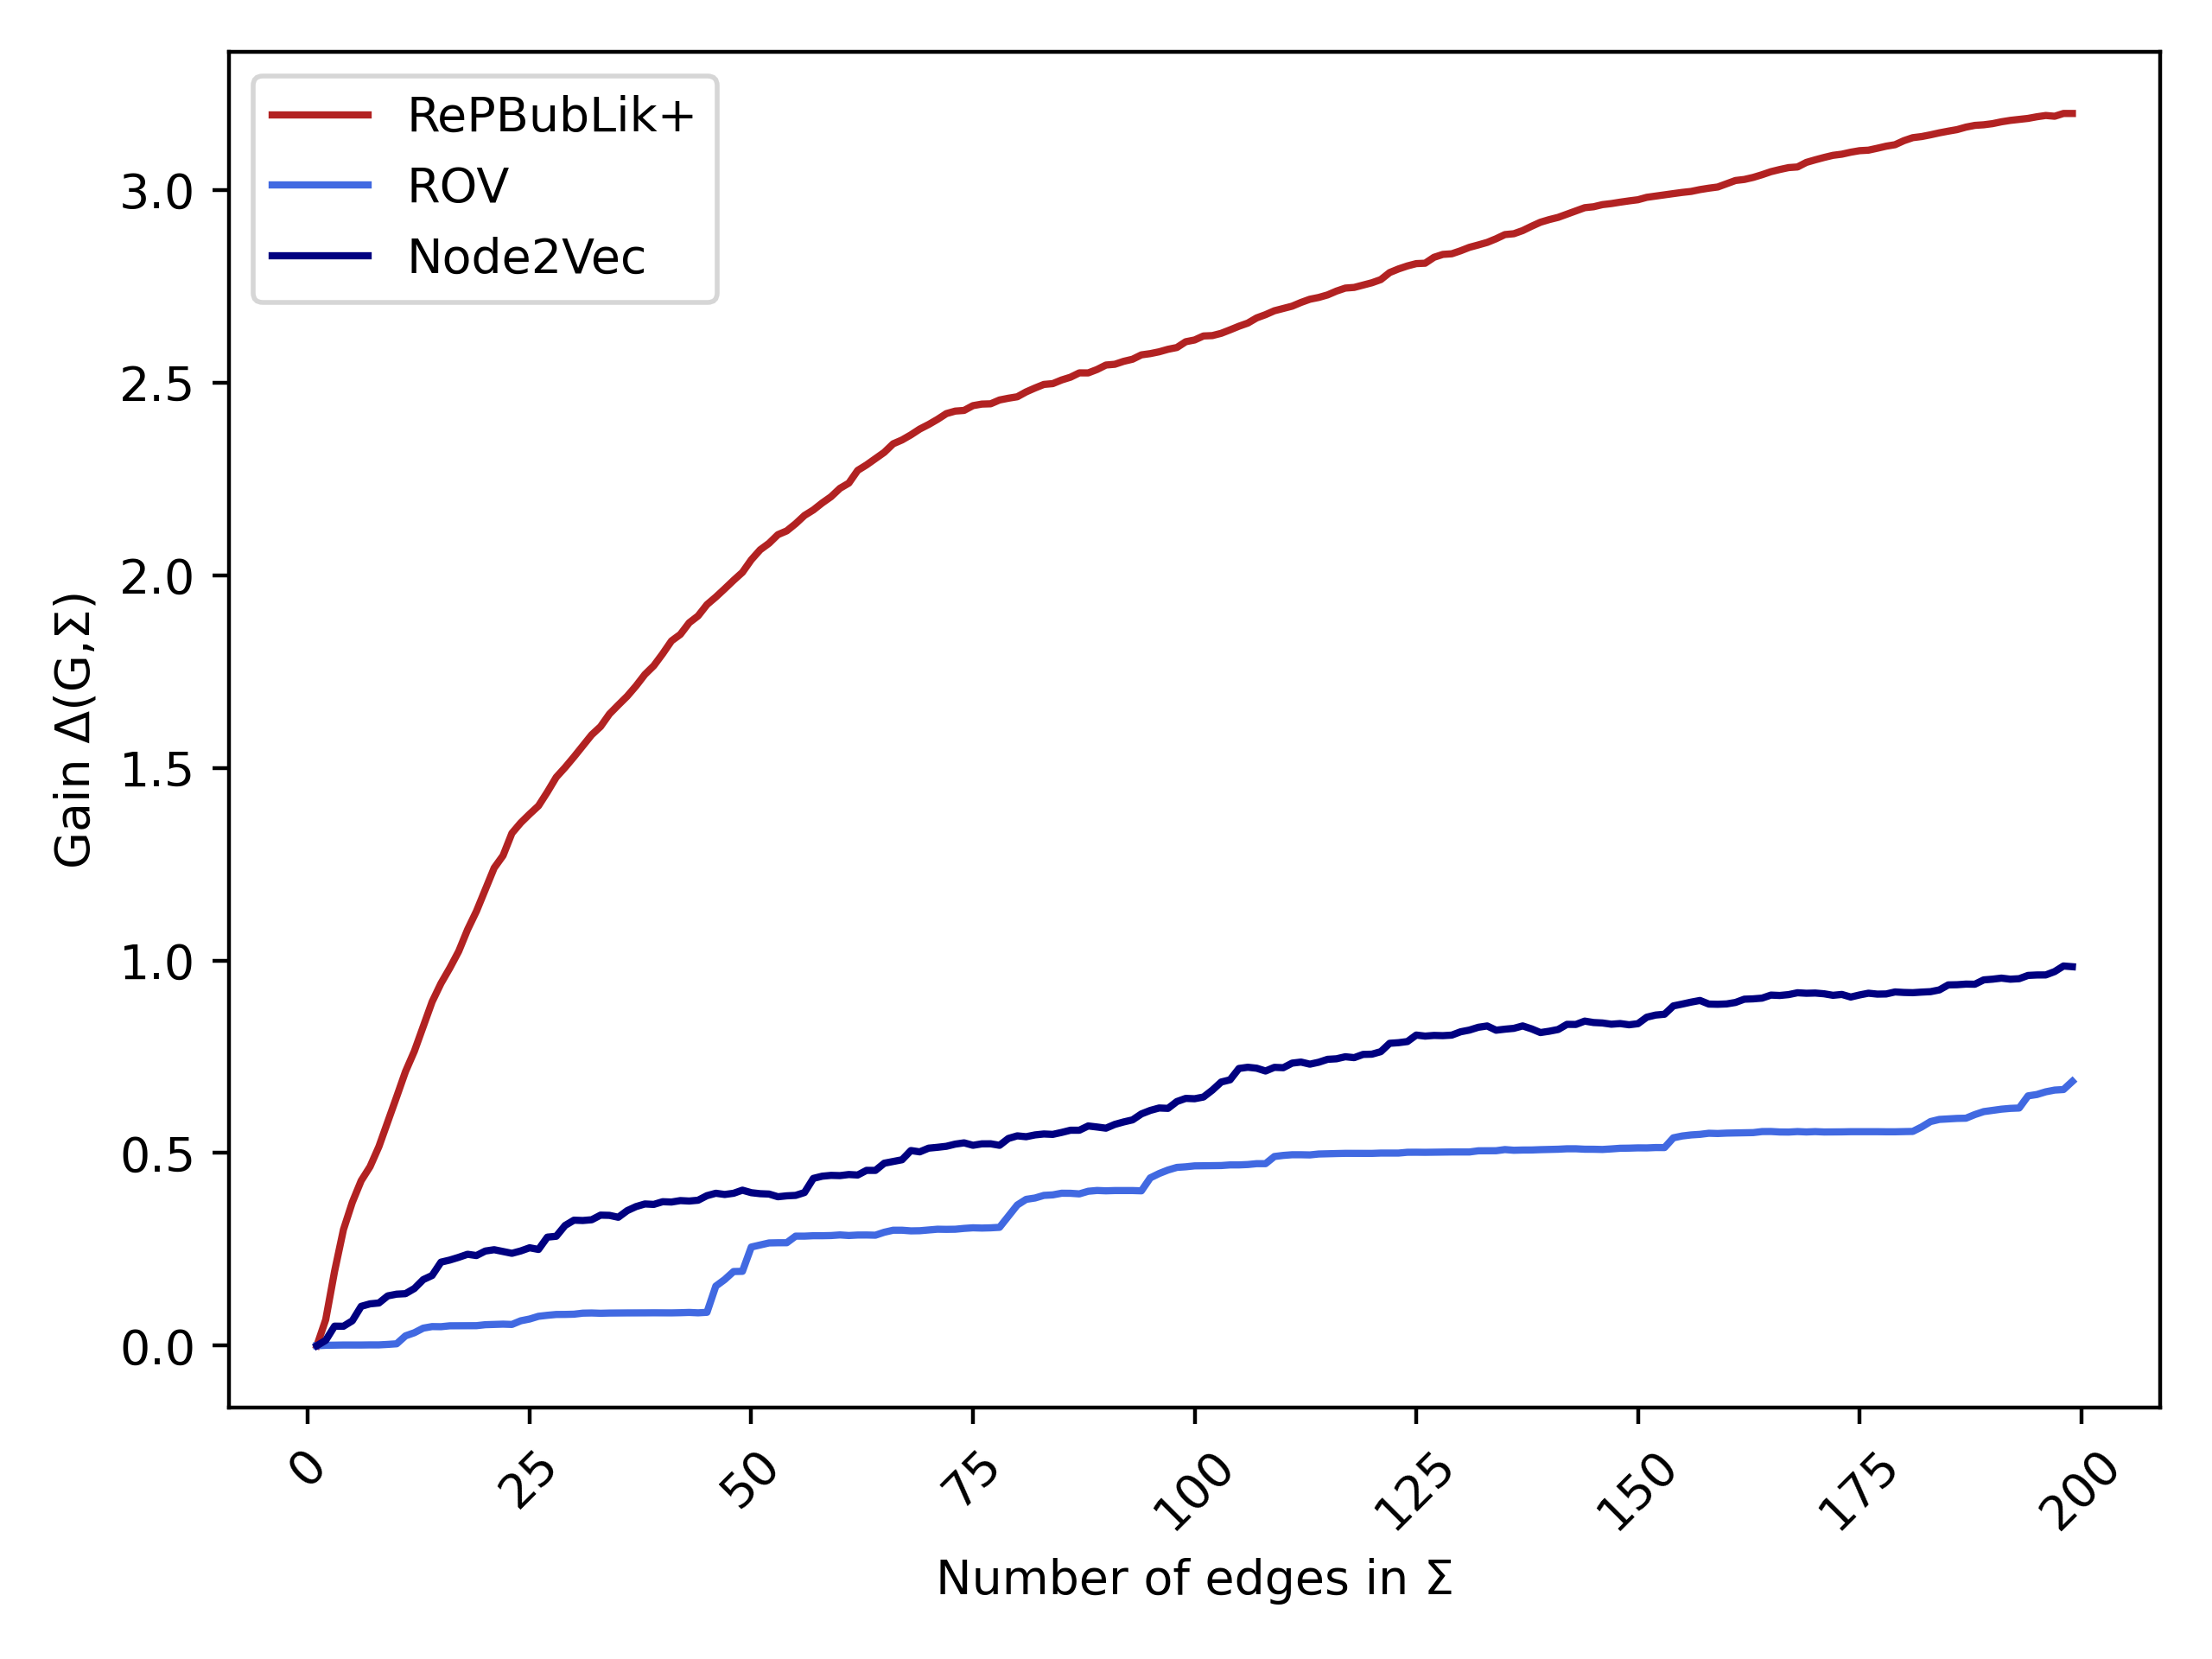
\includegraphics[width=\columnwidth]{5/math_tech_gain_5.png}
    \caption{\emph{MaTe} plot}\label{fig:mate_g_5}
\end{subfigure}
\hspace{0.1\columnwidth}
\begin{subfigure}[h]{0.4\textwidth}
    \centering
    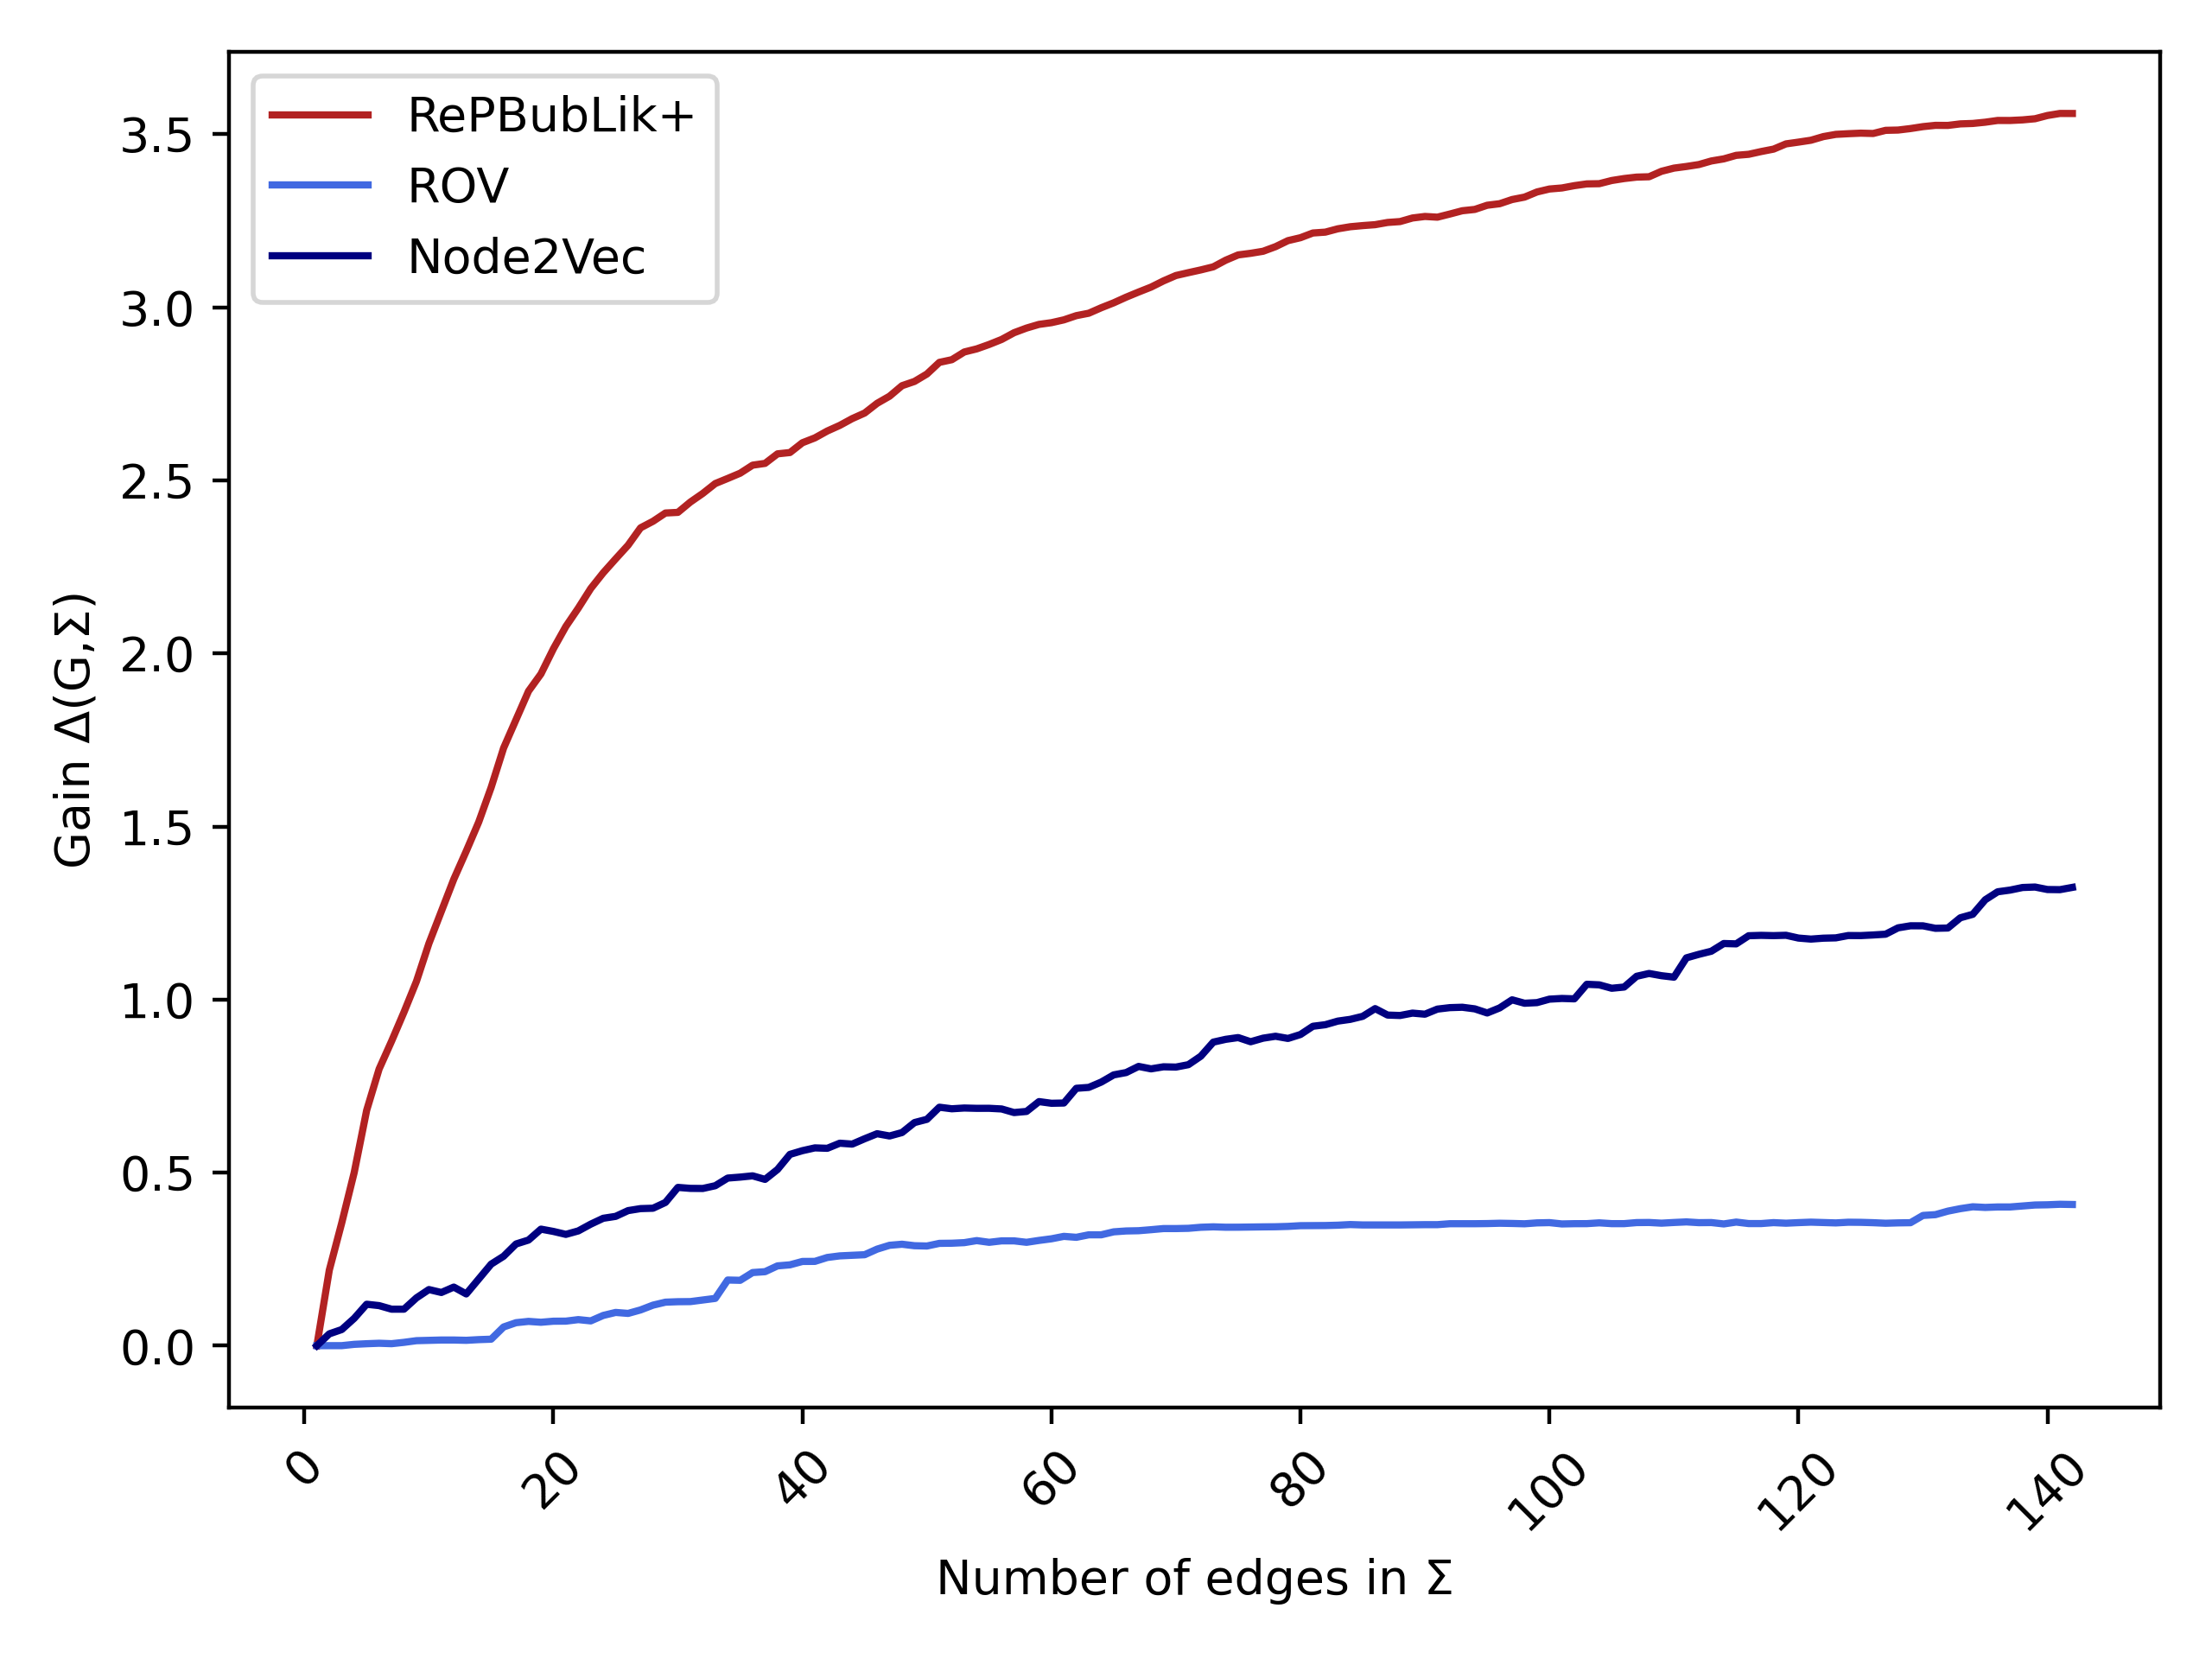
\includegraphics[width=\columnwidth]{5/tech_mil_gain_5.png}
    \caption{\emph{MiHi} plot}\label{fig:mihi_g_5}
\end{subfigure}
\end{figure}
\begin{figure}
    \ContinuedFloat
    \centering
\begin{subfigure}[h]{0.4\textwidth}
    \centering
    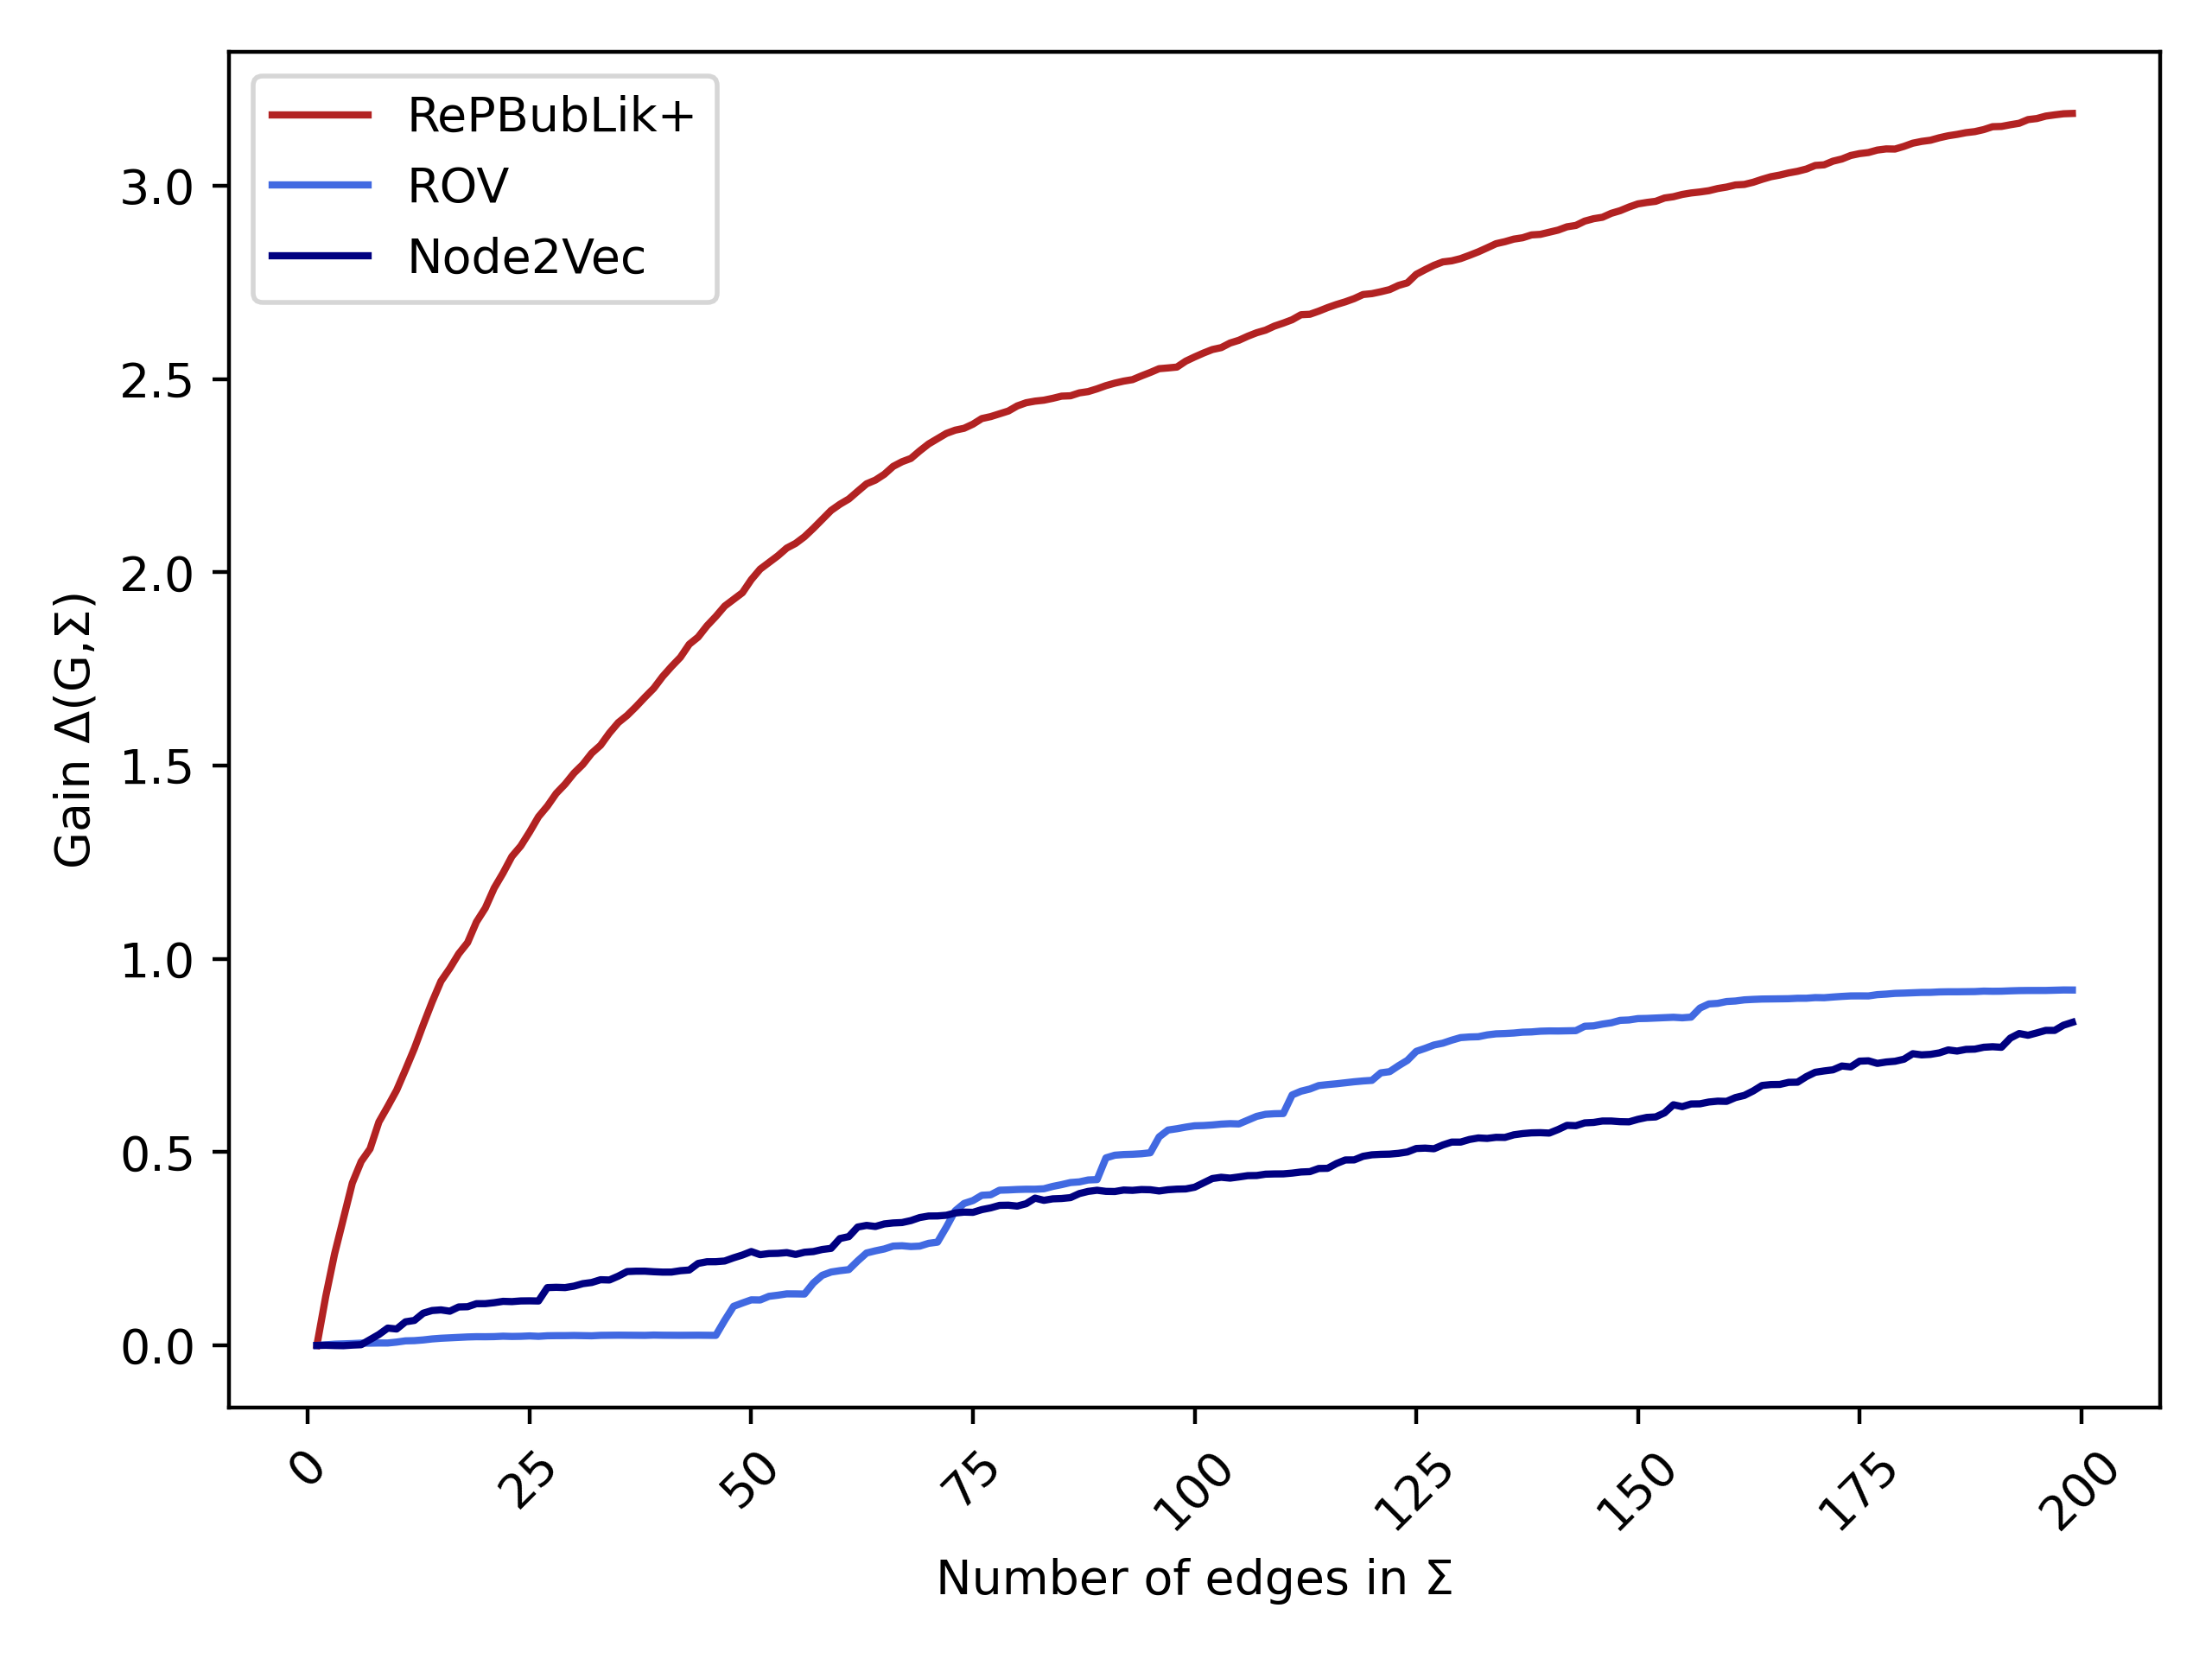
\includegraphics[width=\columnwidth]{5/math_ast_gain_5.png}
    \caption{\emph{MaA}s plot}\label{fig:maas_g_5}
\end{subfigure}
\hspace{0.1\columnwidth}
\begin{subfigure}[h]{0.4\textwidth}
    \centering
    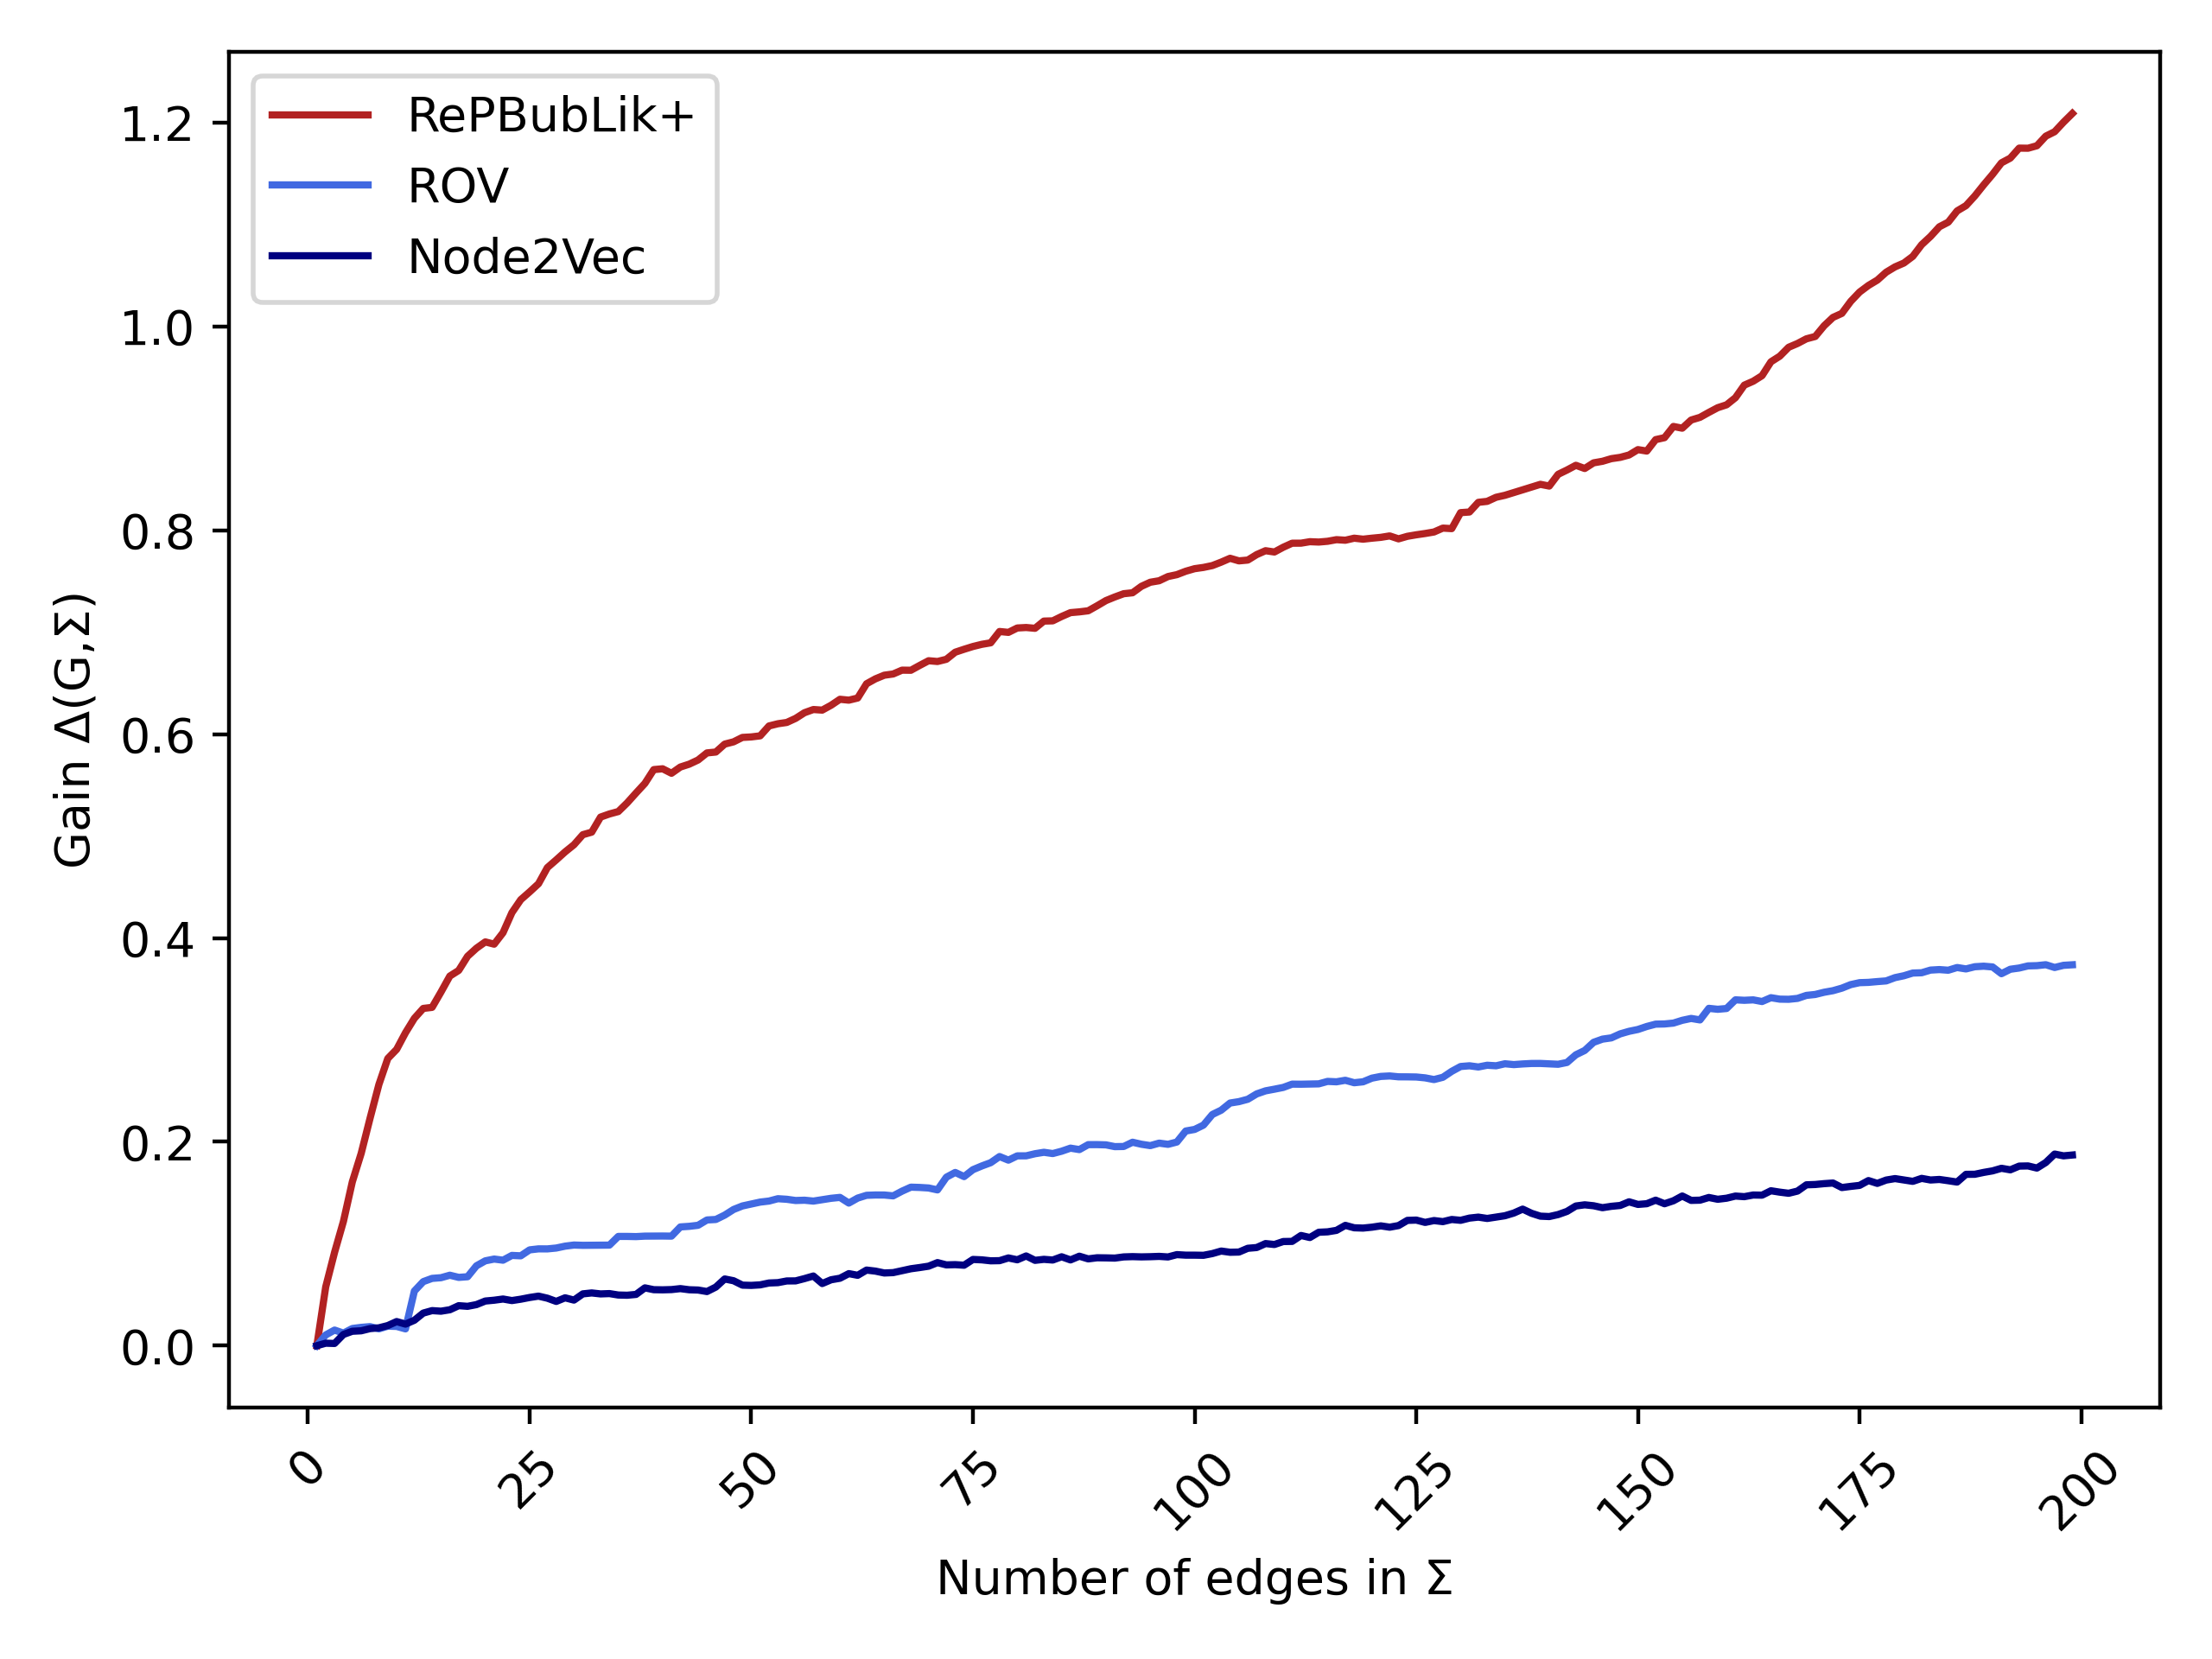
\includegraphics[width=\columnwidth]{5/polblogs_gain_5.png}
    \caption{\emph{PolBlogs} plot}\label{fig:polblogs_g_5}
\end{subfigure}
\caption{Grafici $\Delta(G,\Sigma)$ per $t=5$}
\end{figure}
\begin{figure}[!h]
    \centering
\begin{subfigure}[b]{0.4\textwidth}
    \centering
    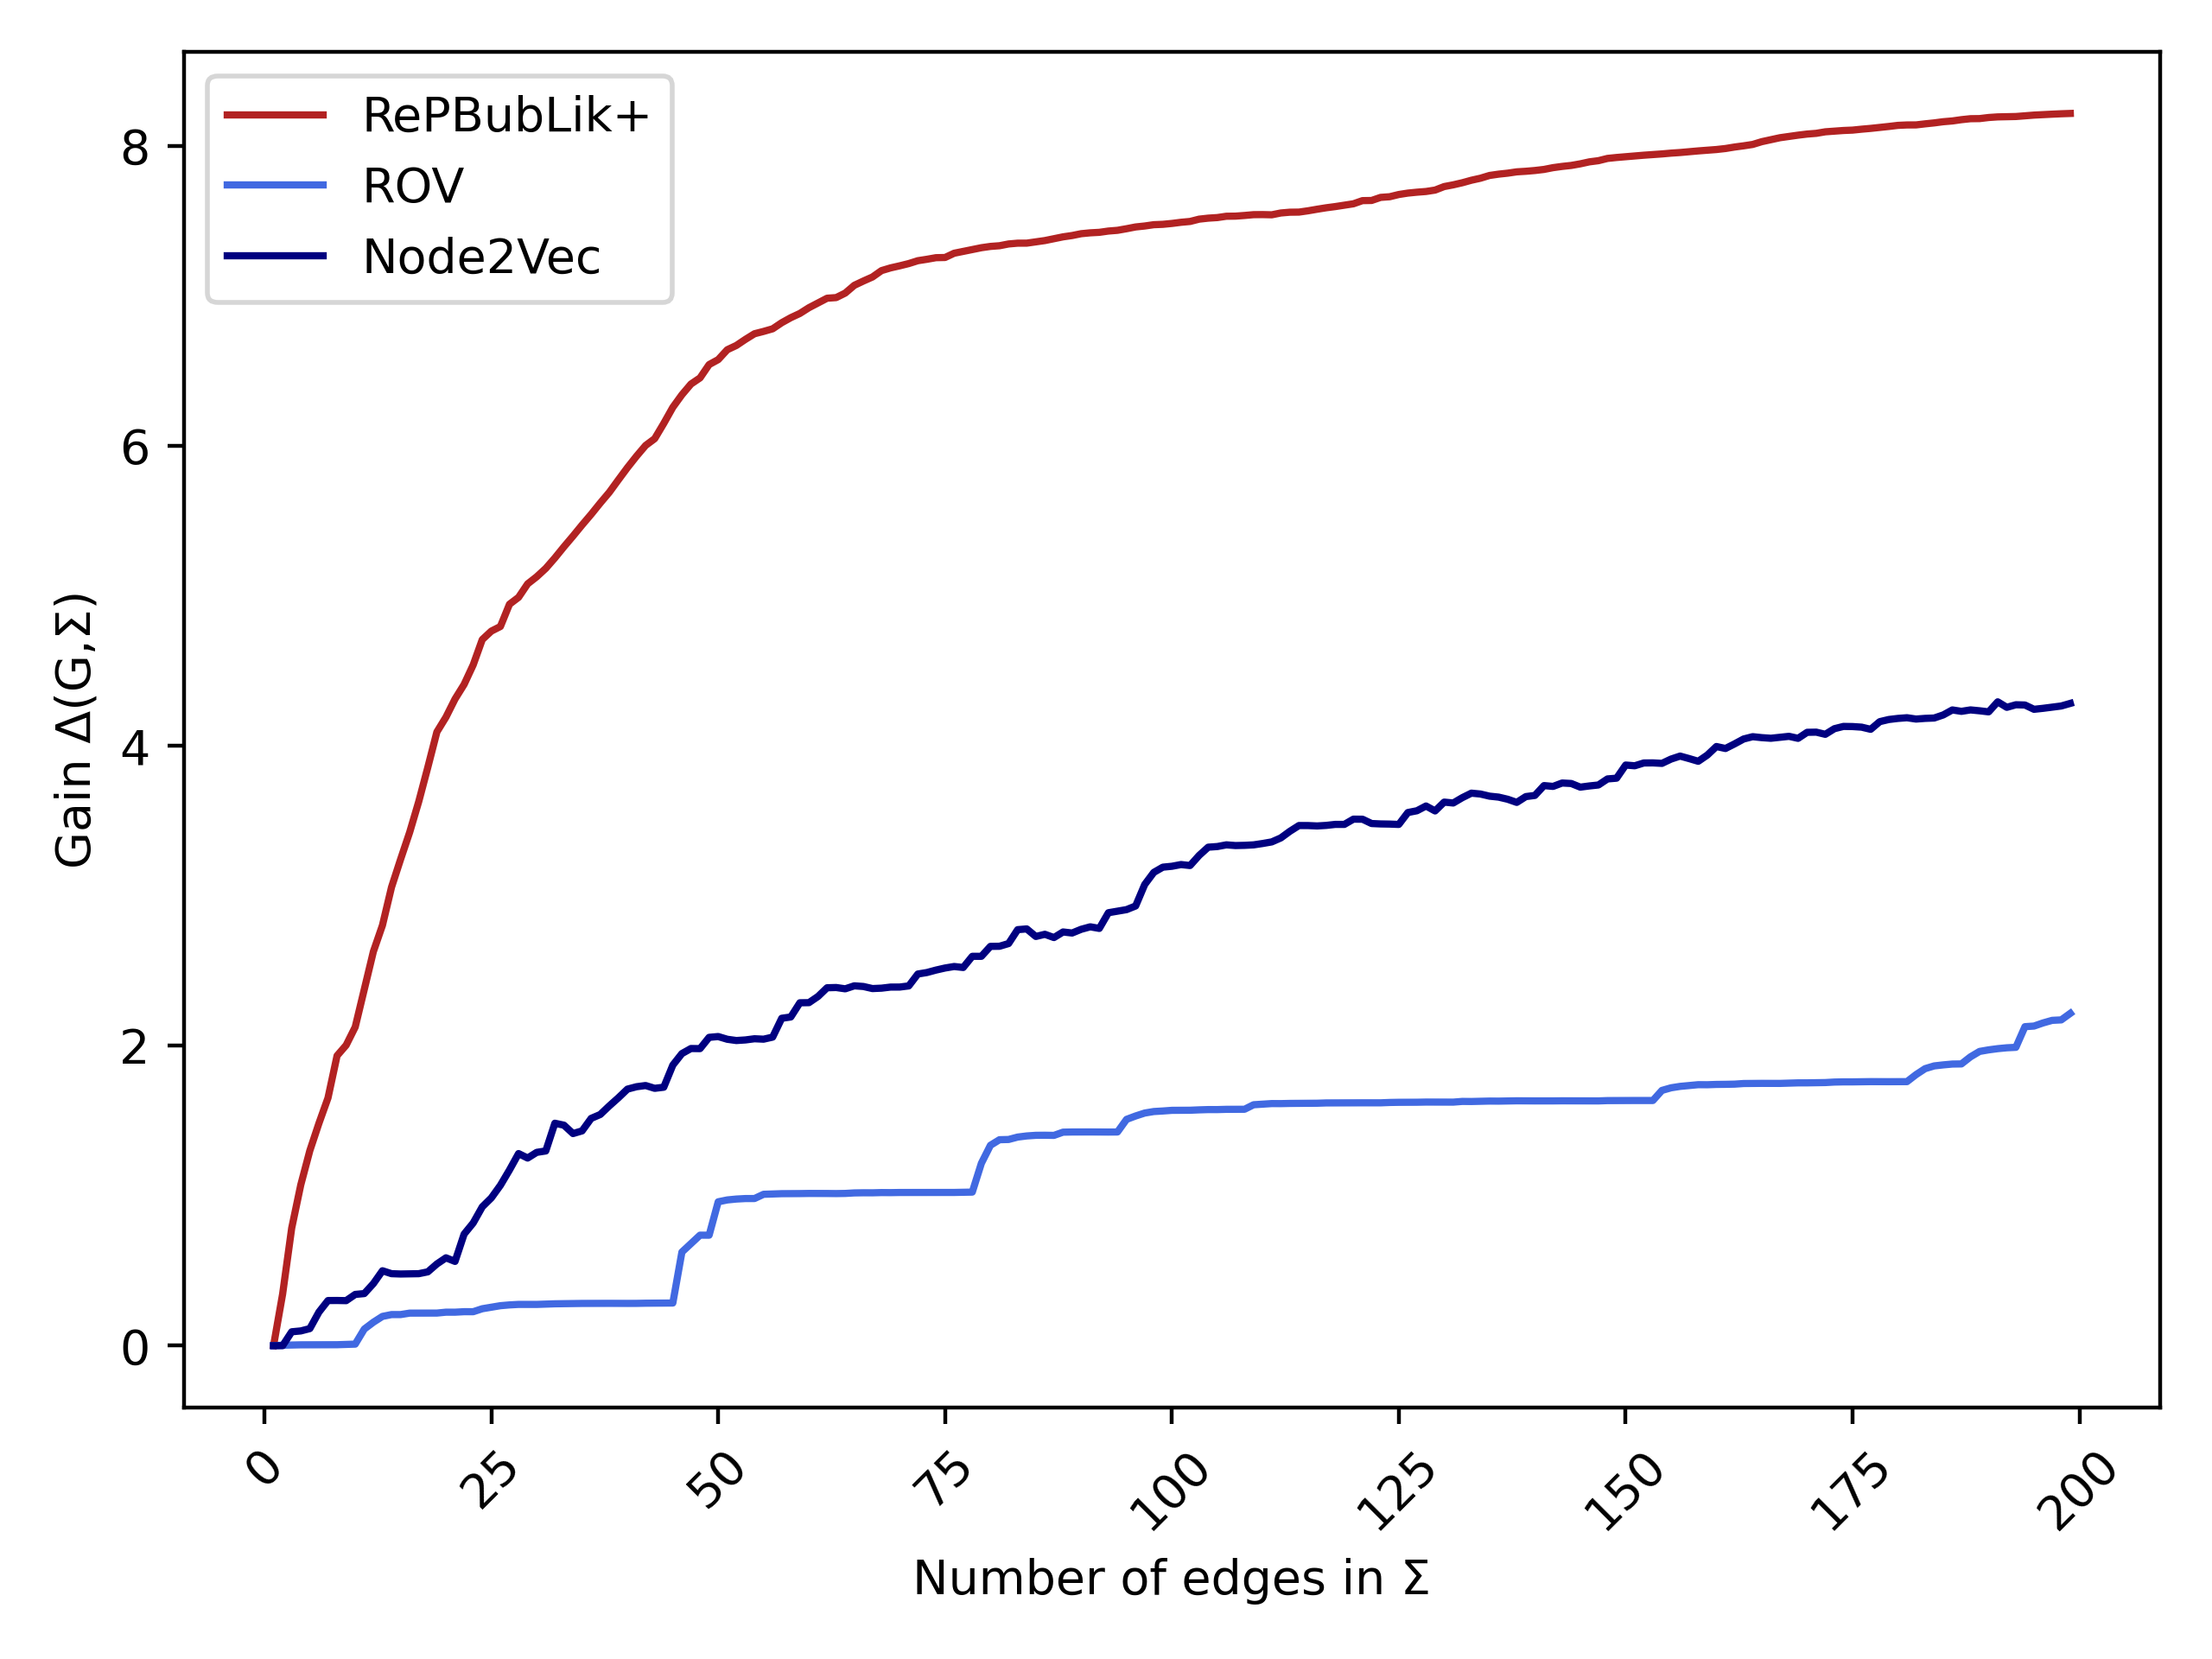
\includegraphics[width=\columnwidth]{10/math_tech_gain_10.png}
    \caption{\emph{MaTe} plot}\label{fig:mate_g_10}
\end{subfigure}
\hspace{0.1\columnwidth}
\begin{subfigure}[b]{0.4\textwidth}
    \centering
    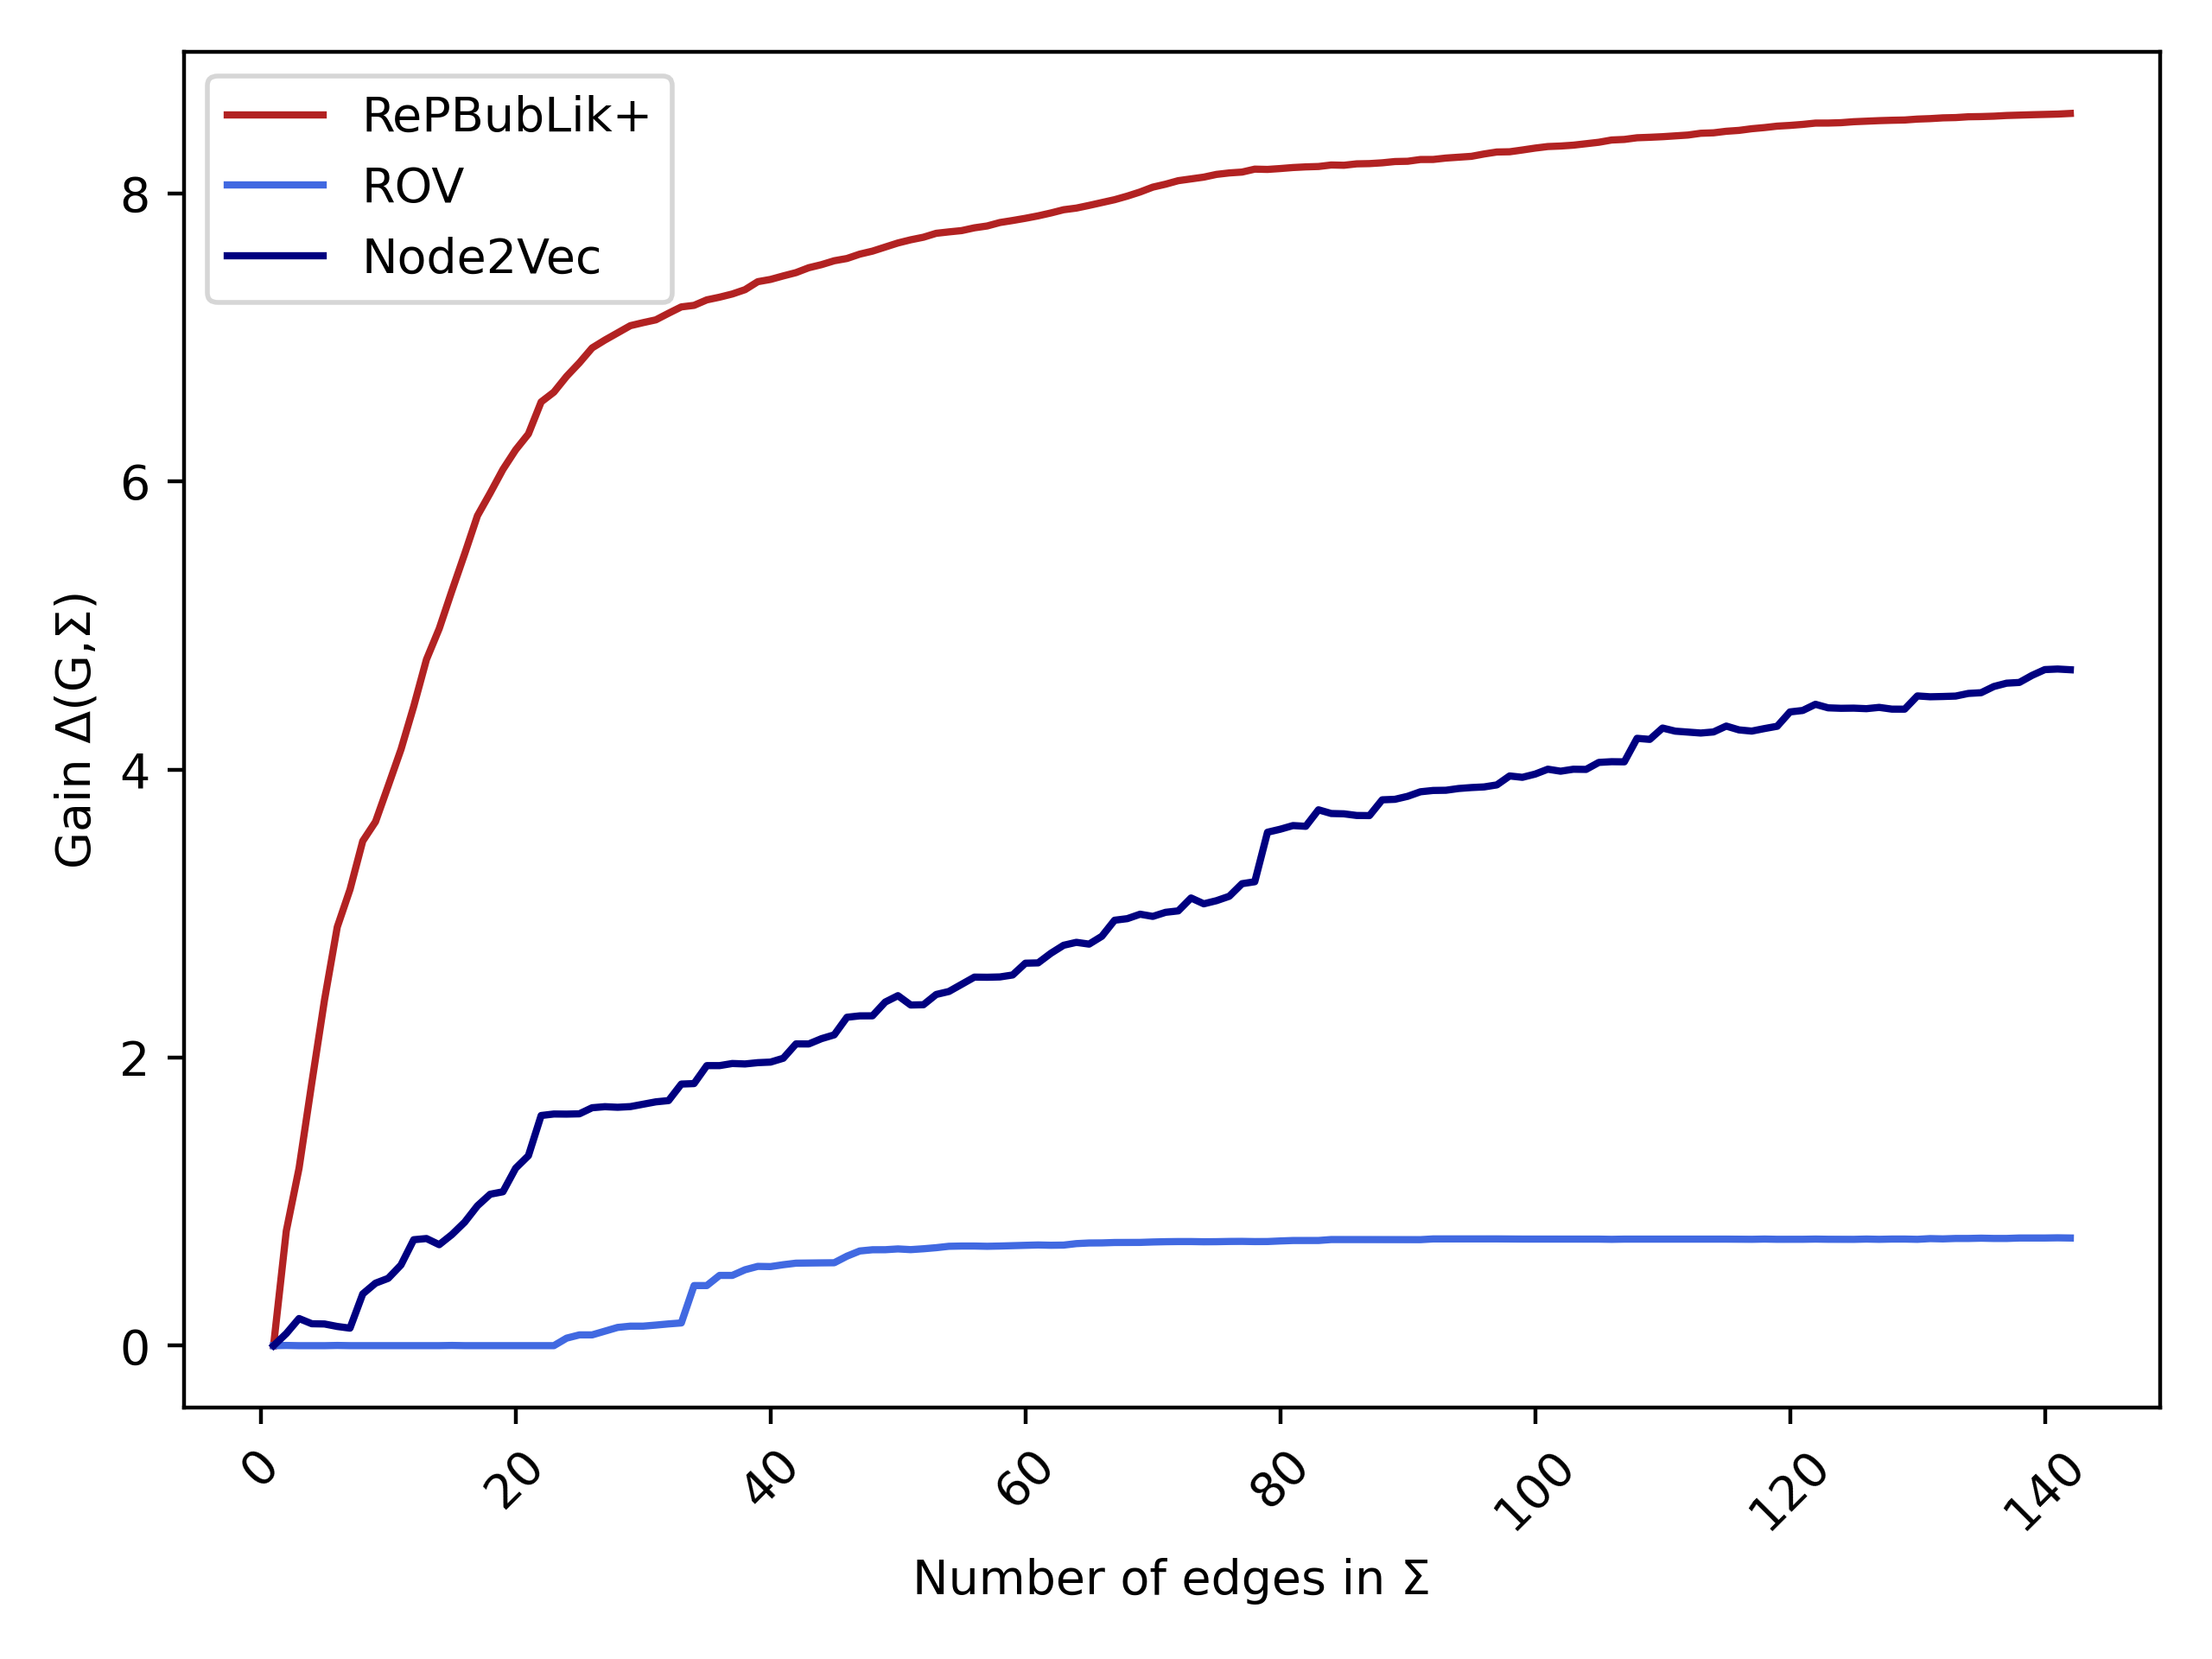
\includegraphics[width=\columnwidth]{10/tech_mil_gain_10.png}
    \caption{\emph{MiHi} plot}\label{fig:mihi_g_10}
\end{subfigure}

\begin{subfigure}[b]{0.4\textwidth}
    \centering
    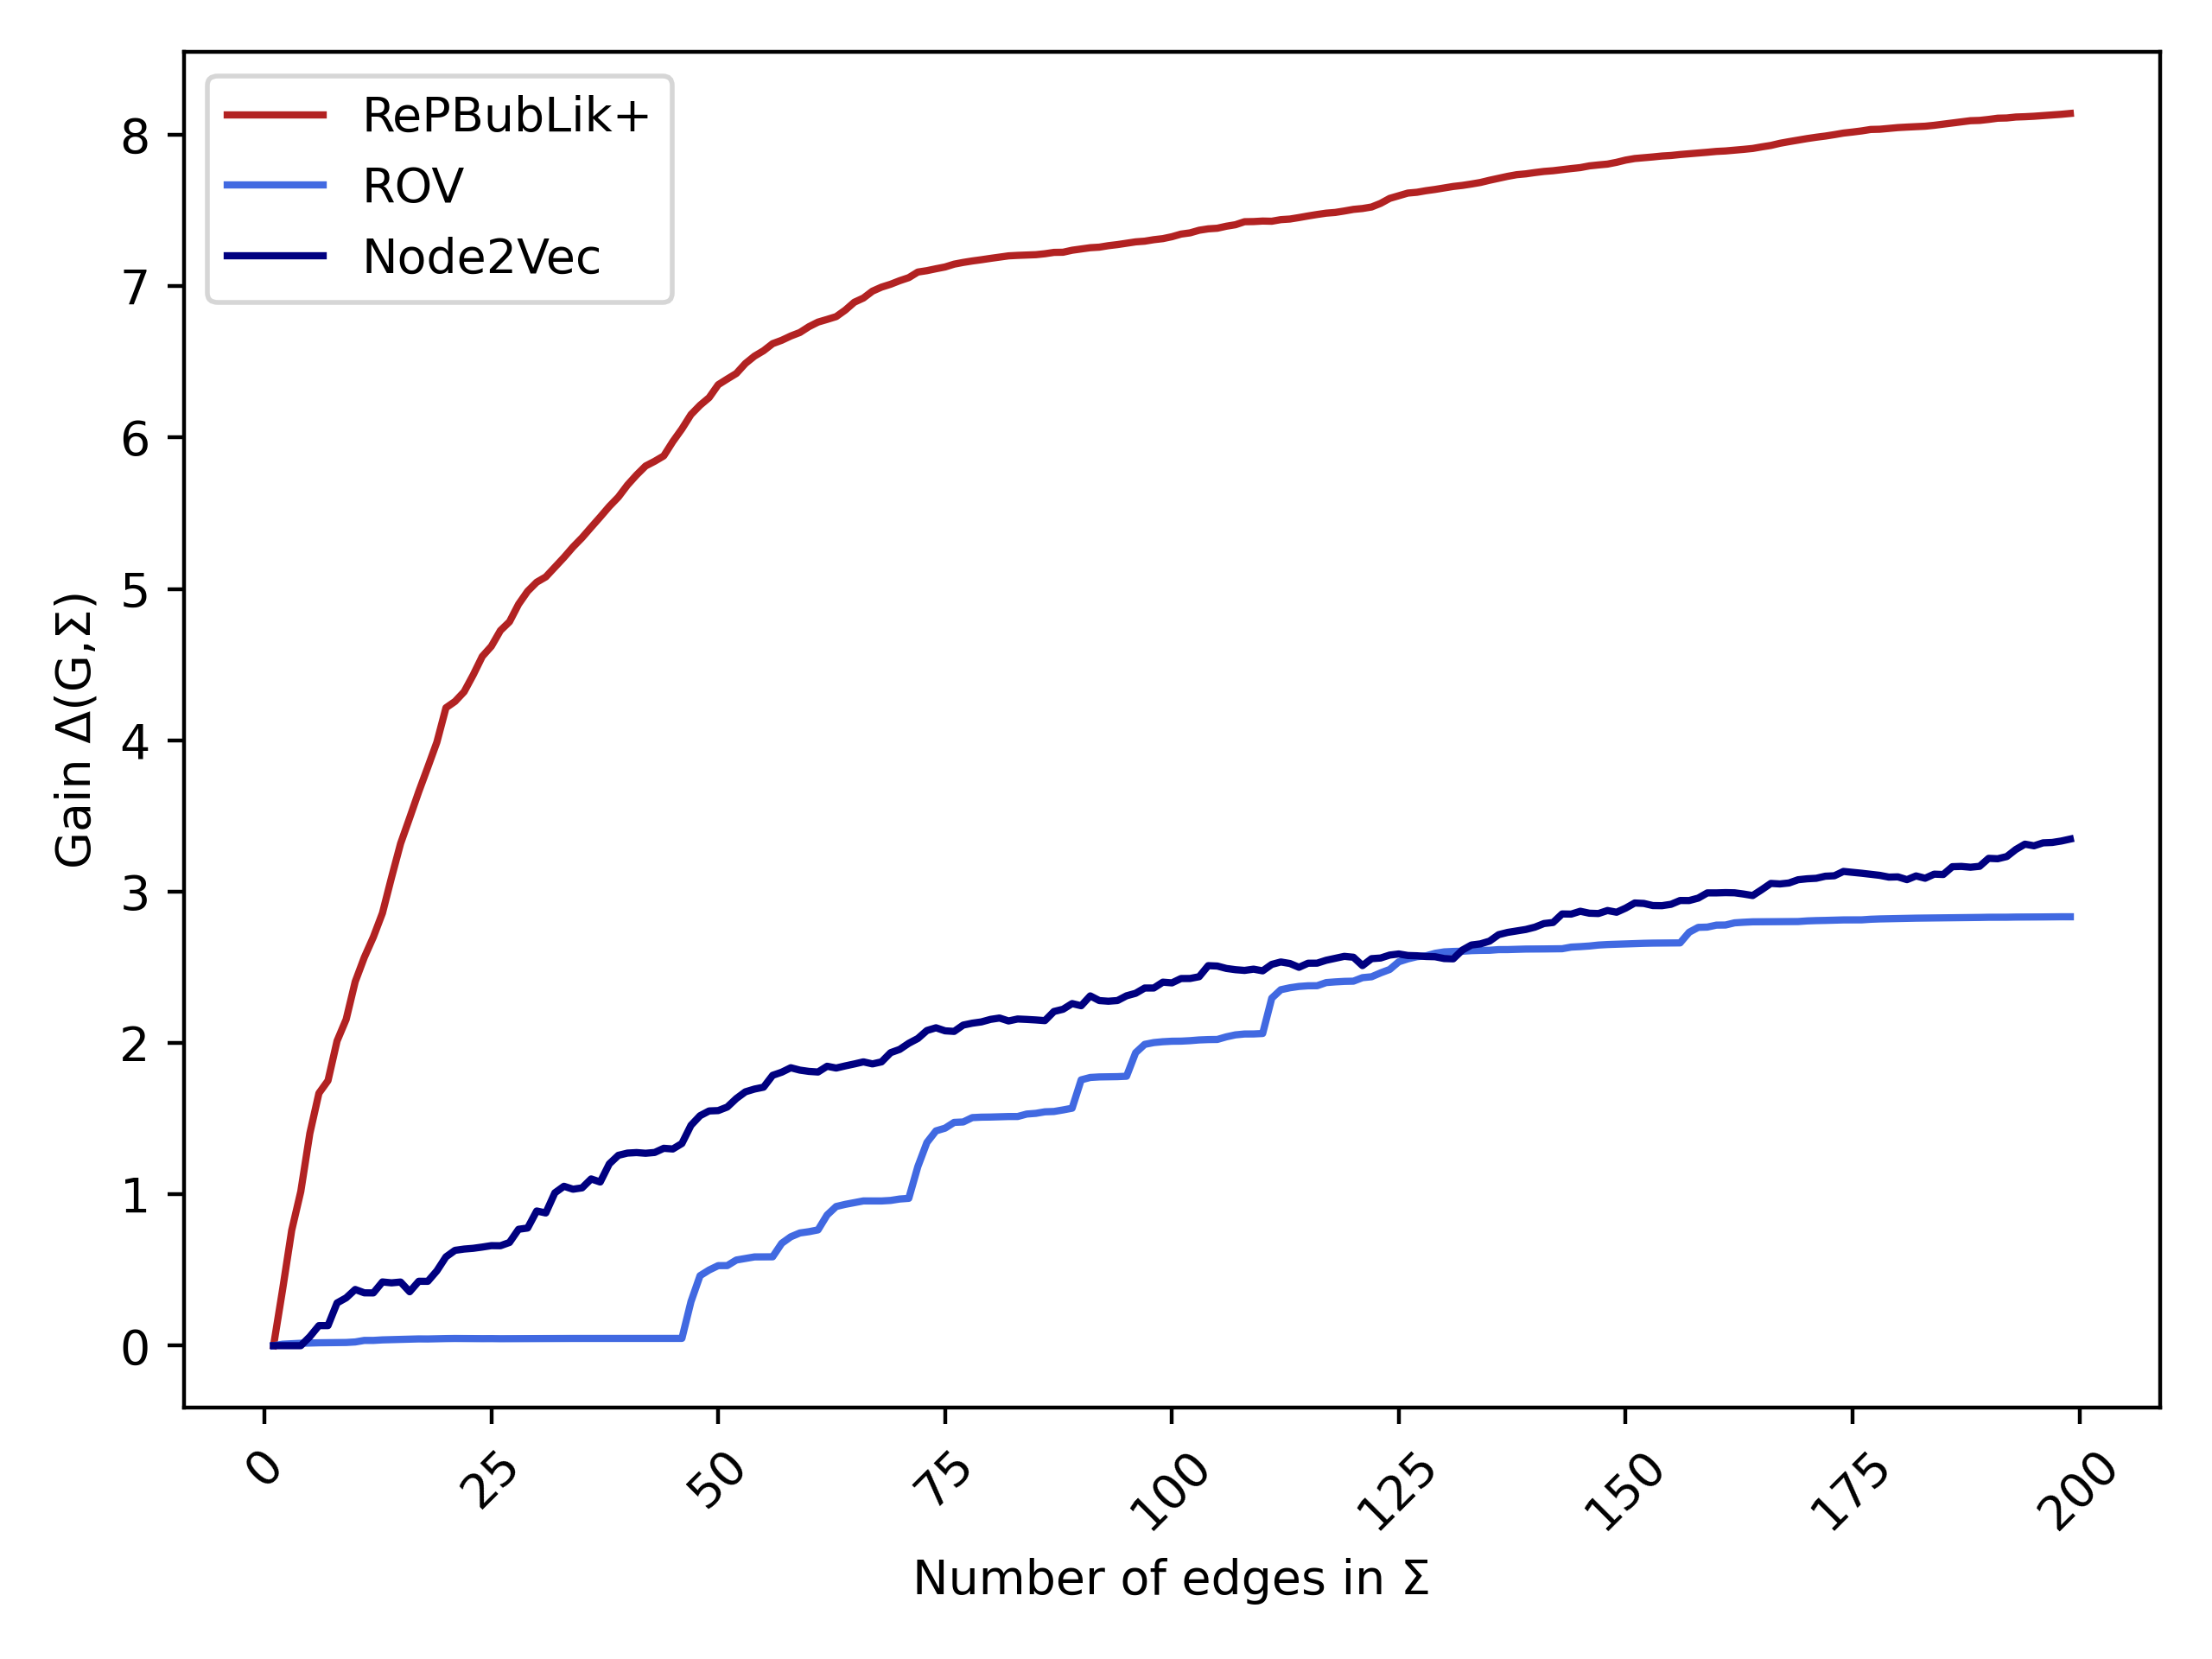
\includegraphics[width=\columnwidth]{10/math_ast_gain_10.png}
    \caption{\emph{MaA}s plot}\label{fig:maas_g_10}
\end{subfigure}
\hspace{0.1\columnwidth}
\begin{subfigure}[b]{0.4\textwidth}
    \centering
    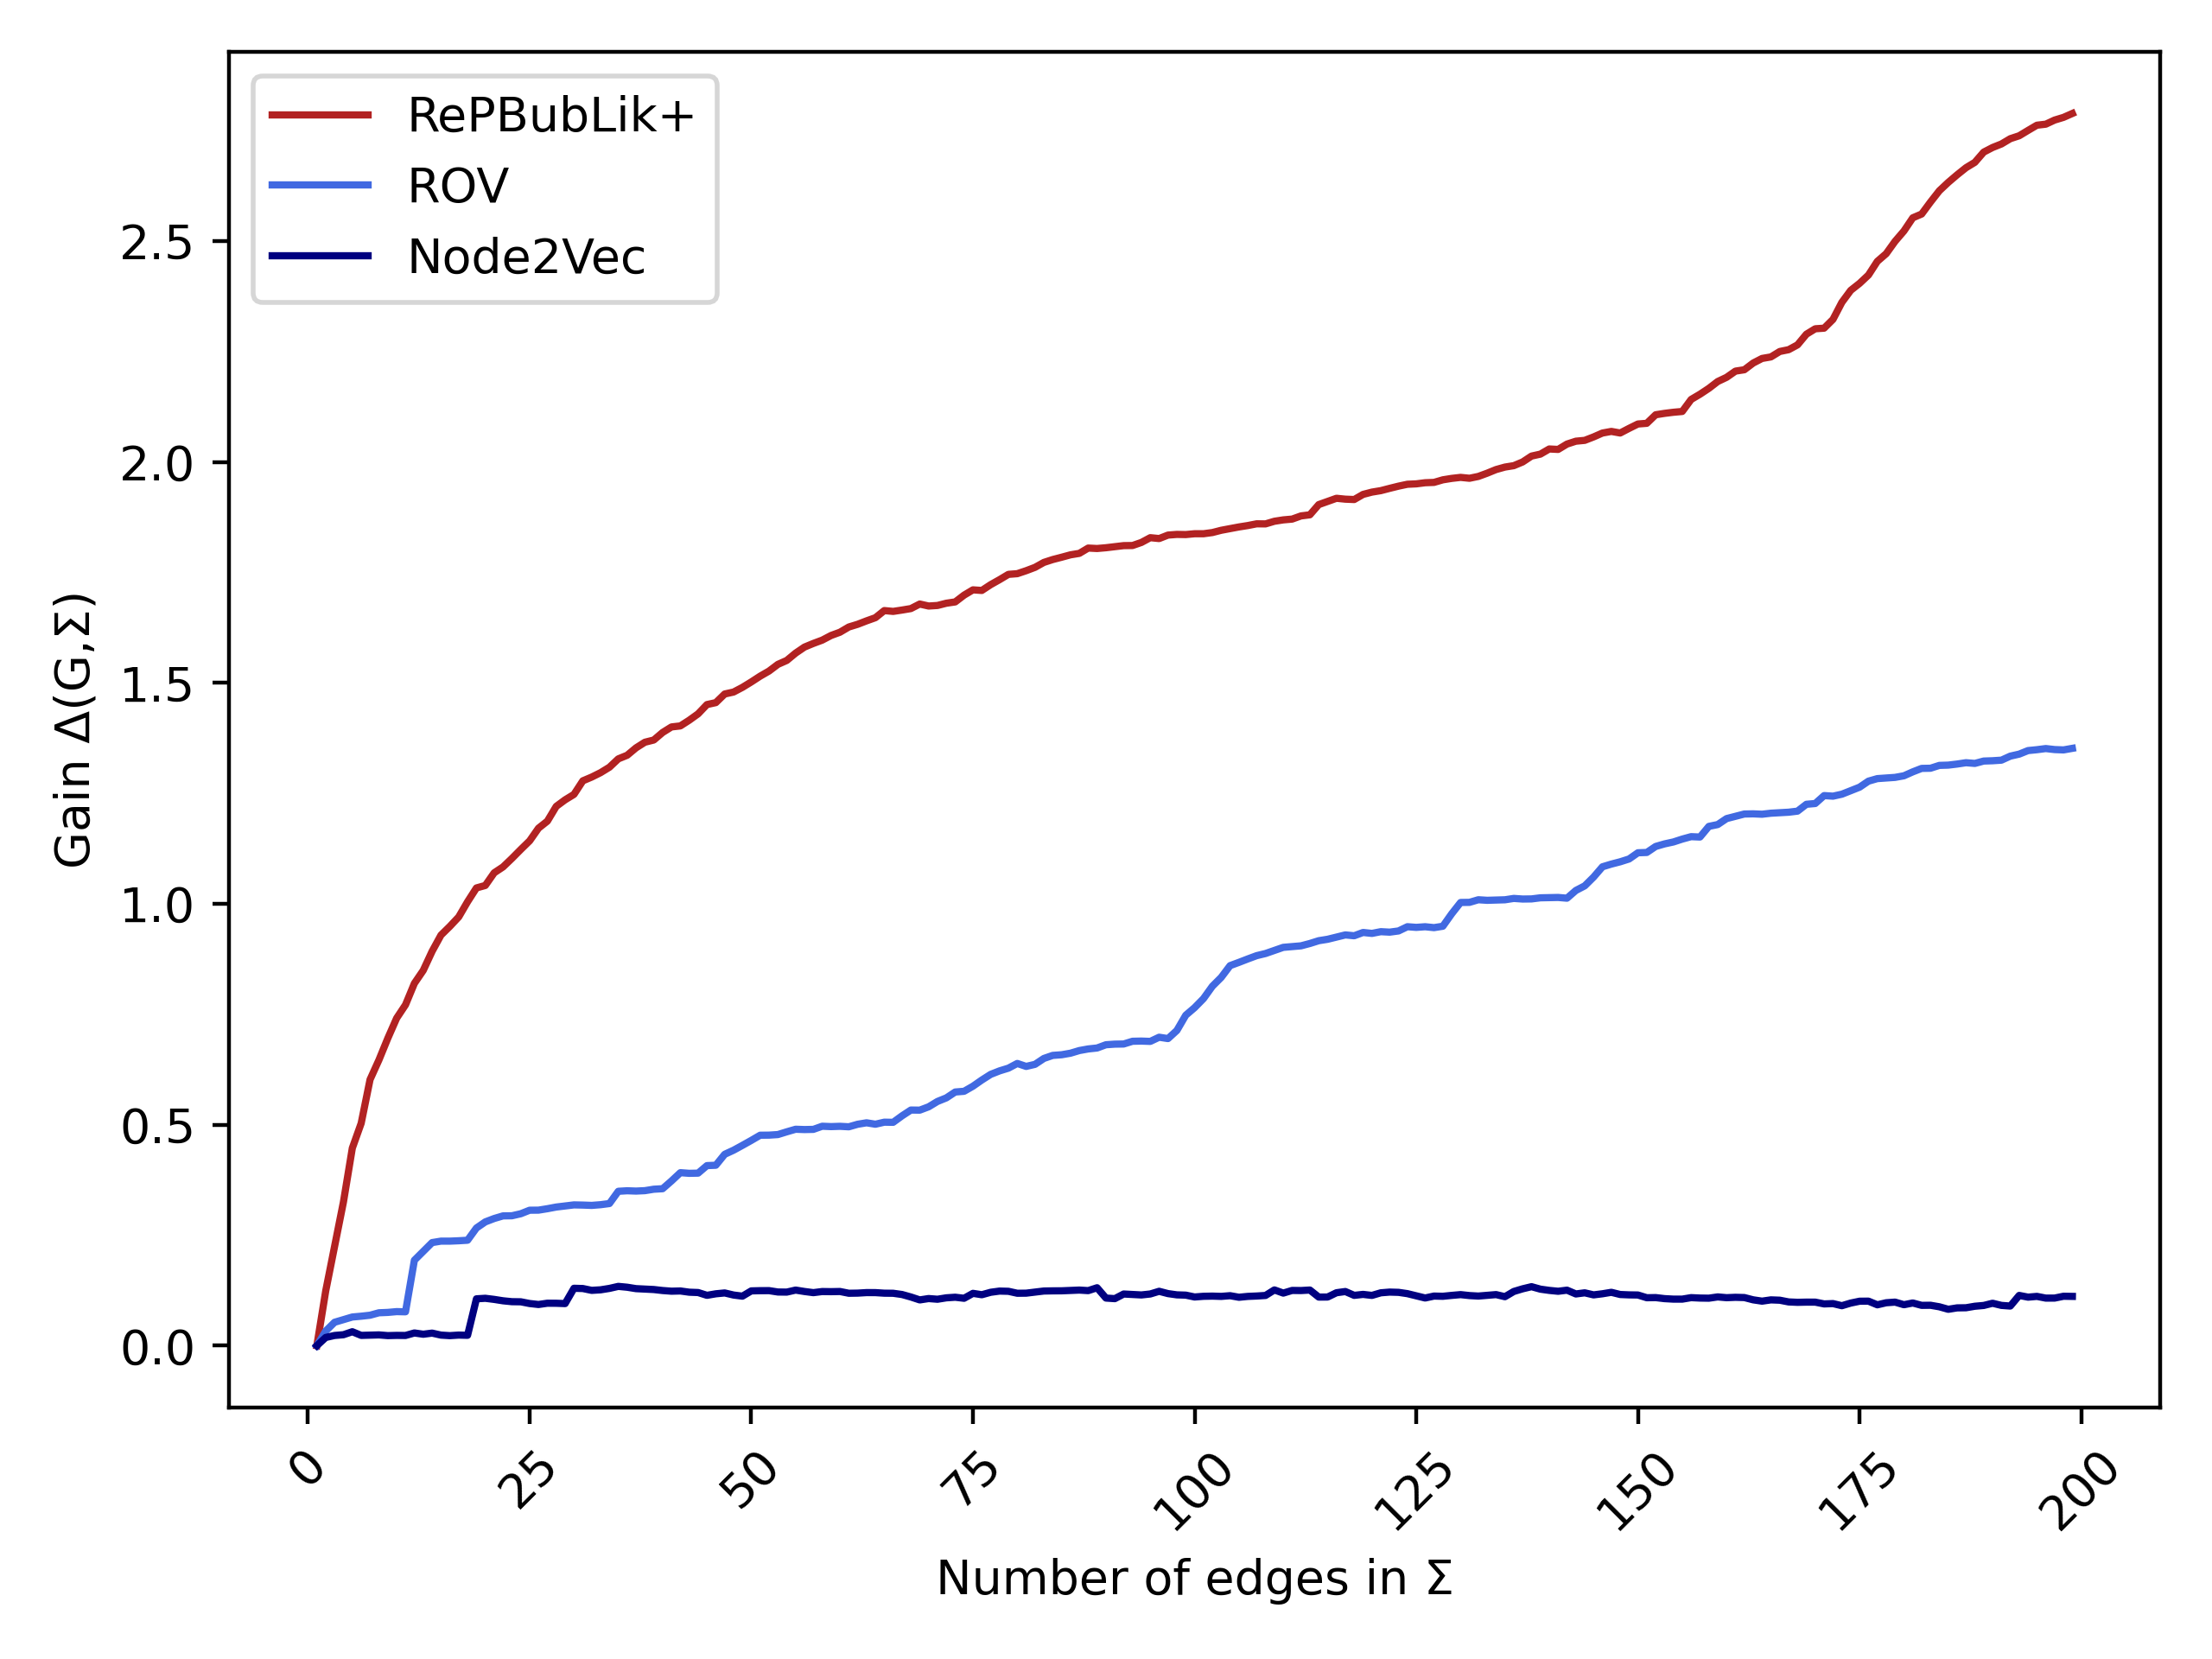
\includegraphics[width=\columnwidth]{10/polblogs_gain_10.png}
    \caption{\emph{PolBlogs} plot}\label{fig:polblogs_g_10}
\end{subfigure}
\caption{Grafici $\Delta(G,\Sigma)$ per $t=10$}
\end{figure}
\newpage
\begin{figure}[!h]
    \centering
\begin{subfigure}[b]{0.4\textwidth}
    \centering
    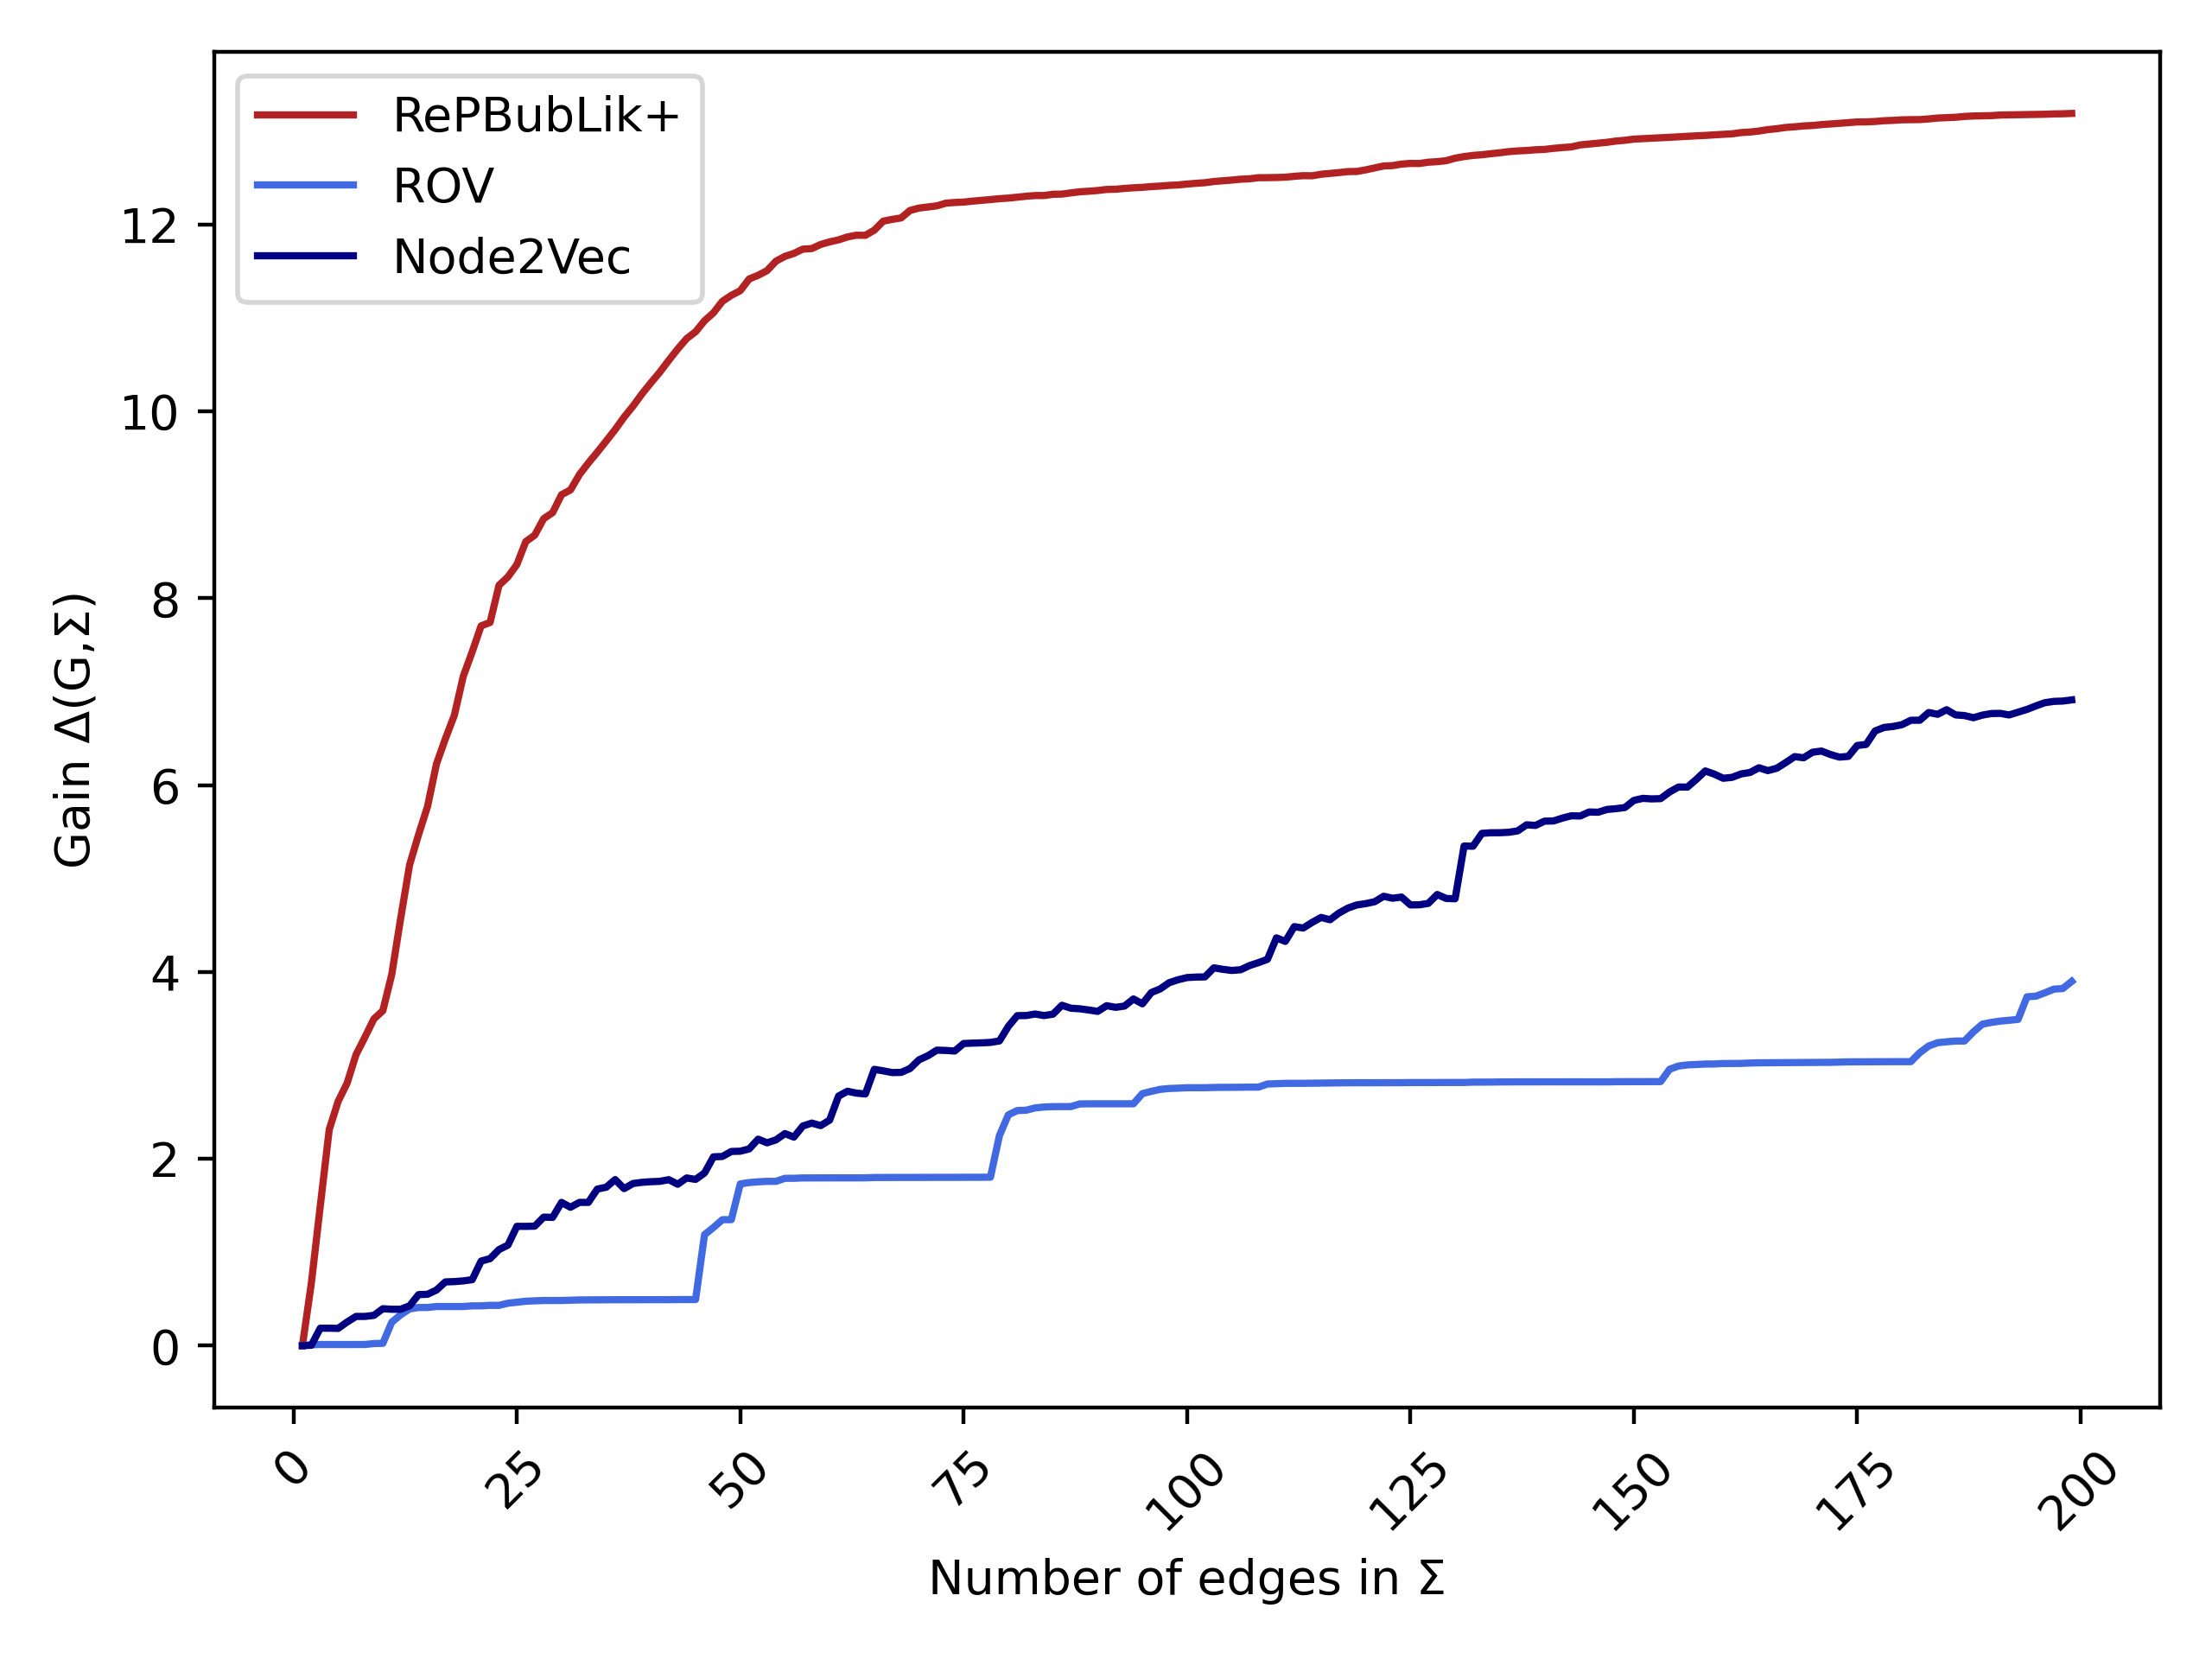
\includegraphics[width=\columnwidth]{15/math_tech_gain_15.png}
    \caption{\emph{MaTe} plot}\label{fig:mate_g_15}
\end{subfigure}
\hspace{0.1\columnwidth}
\begin{subfigure}[b]{0.4\textwidth}
    \centering
    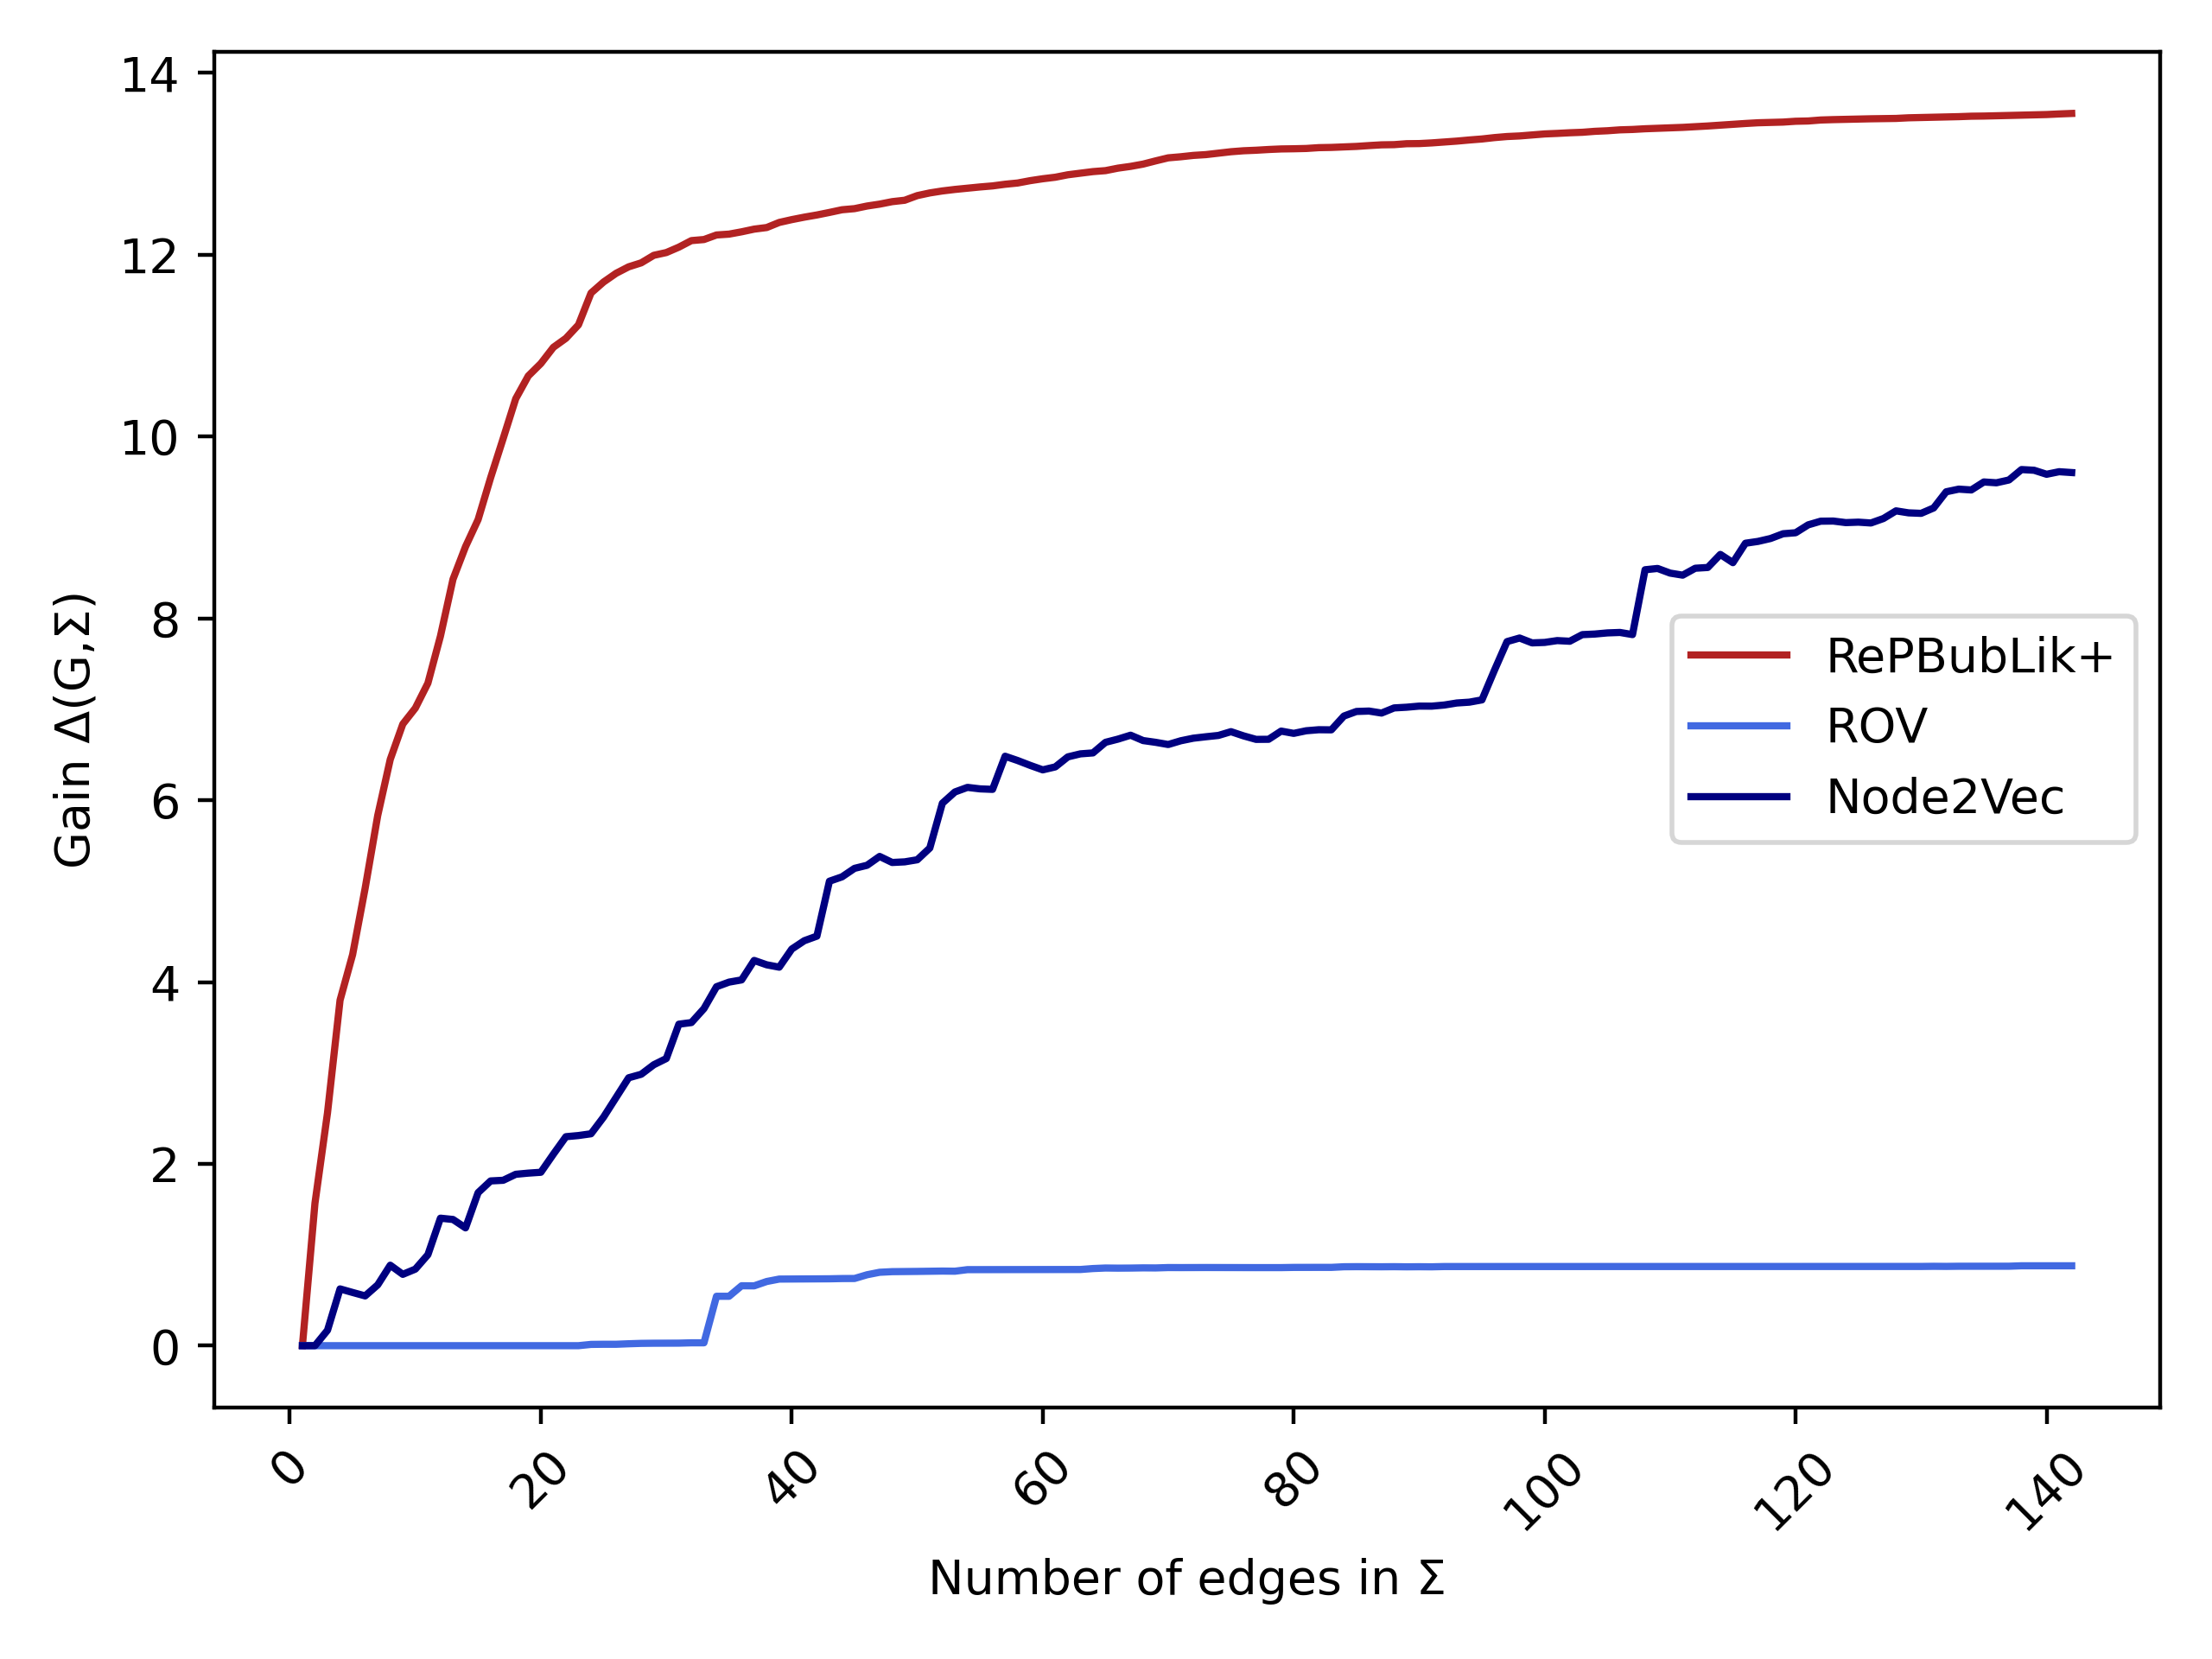
\includegraphics[width=\columnwidth]{15/tech_mil_gain_15.png}
    \caption{\emph{MiHi} plot}\label{fig:mihi_g_15}
\end{subfigure}

\begin{subfigure}[b]{0.4\textwidth}
    \centering
    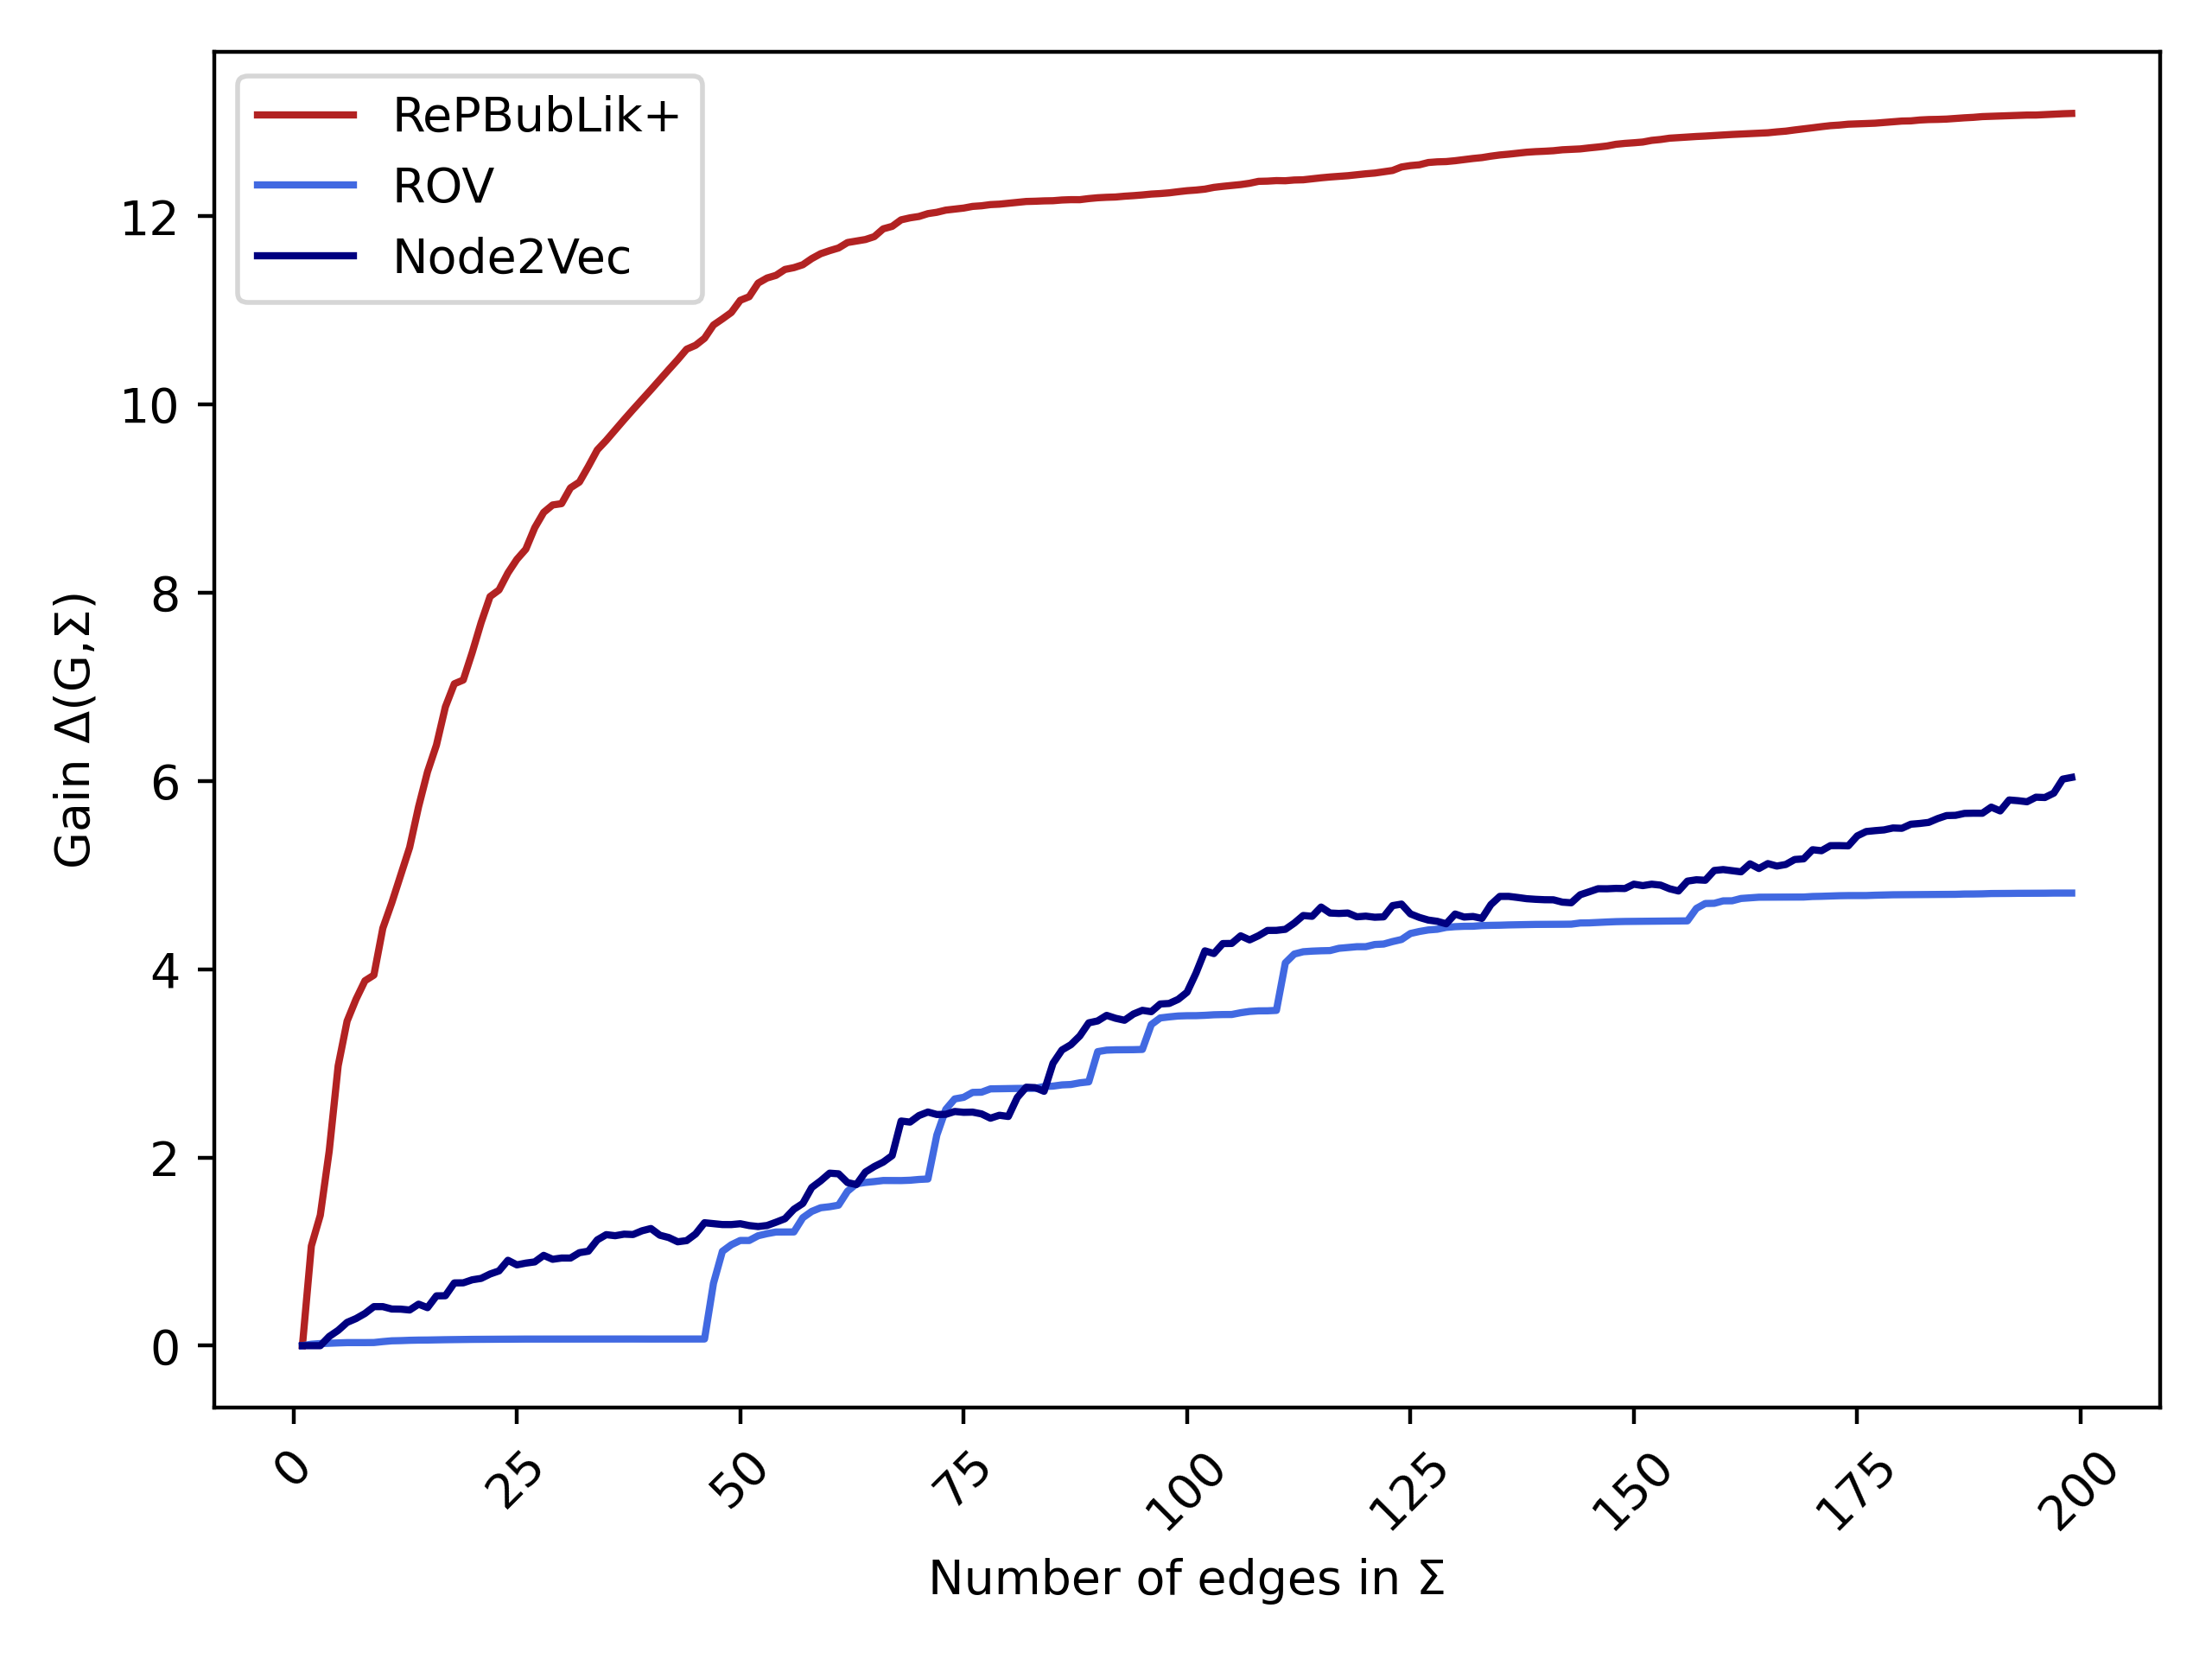
\includegraphics[width=\columnwidth]{15/math_ast_gain_15.png}
    \caption{\emph{MaA}s plot}\label{fig:maas_g_15}
\end{subfigure}
\hspace{0.1\columnwidth}
\begin{subfigure}[b]{0.4\textwidth}
    \centering
    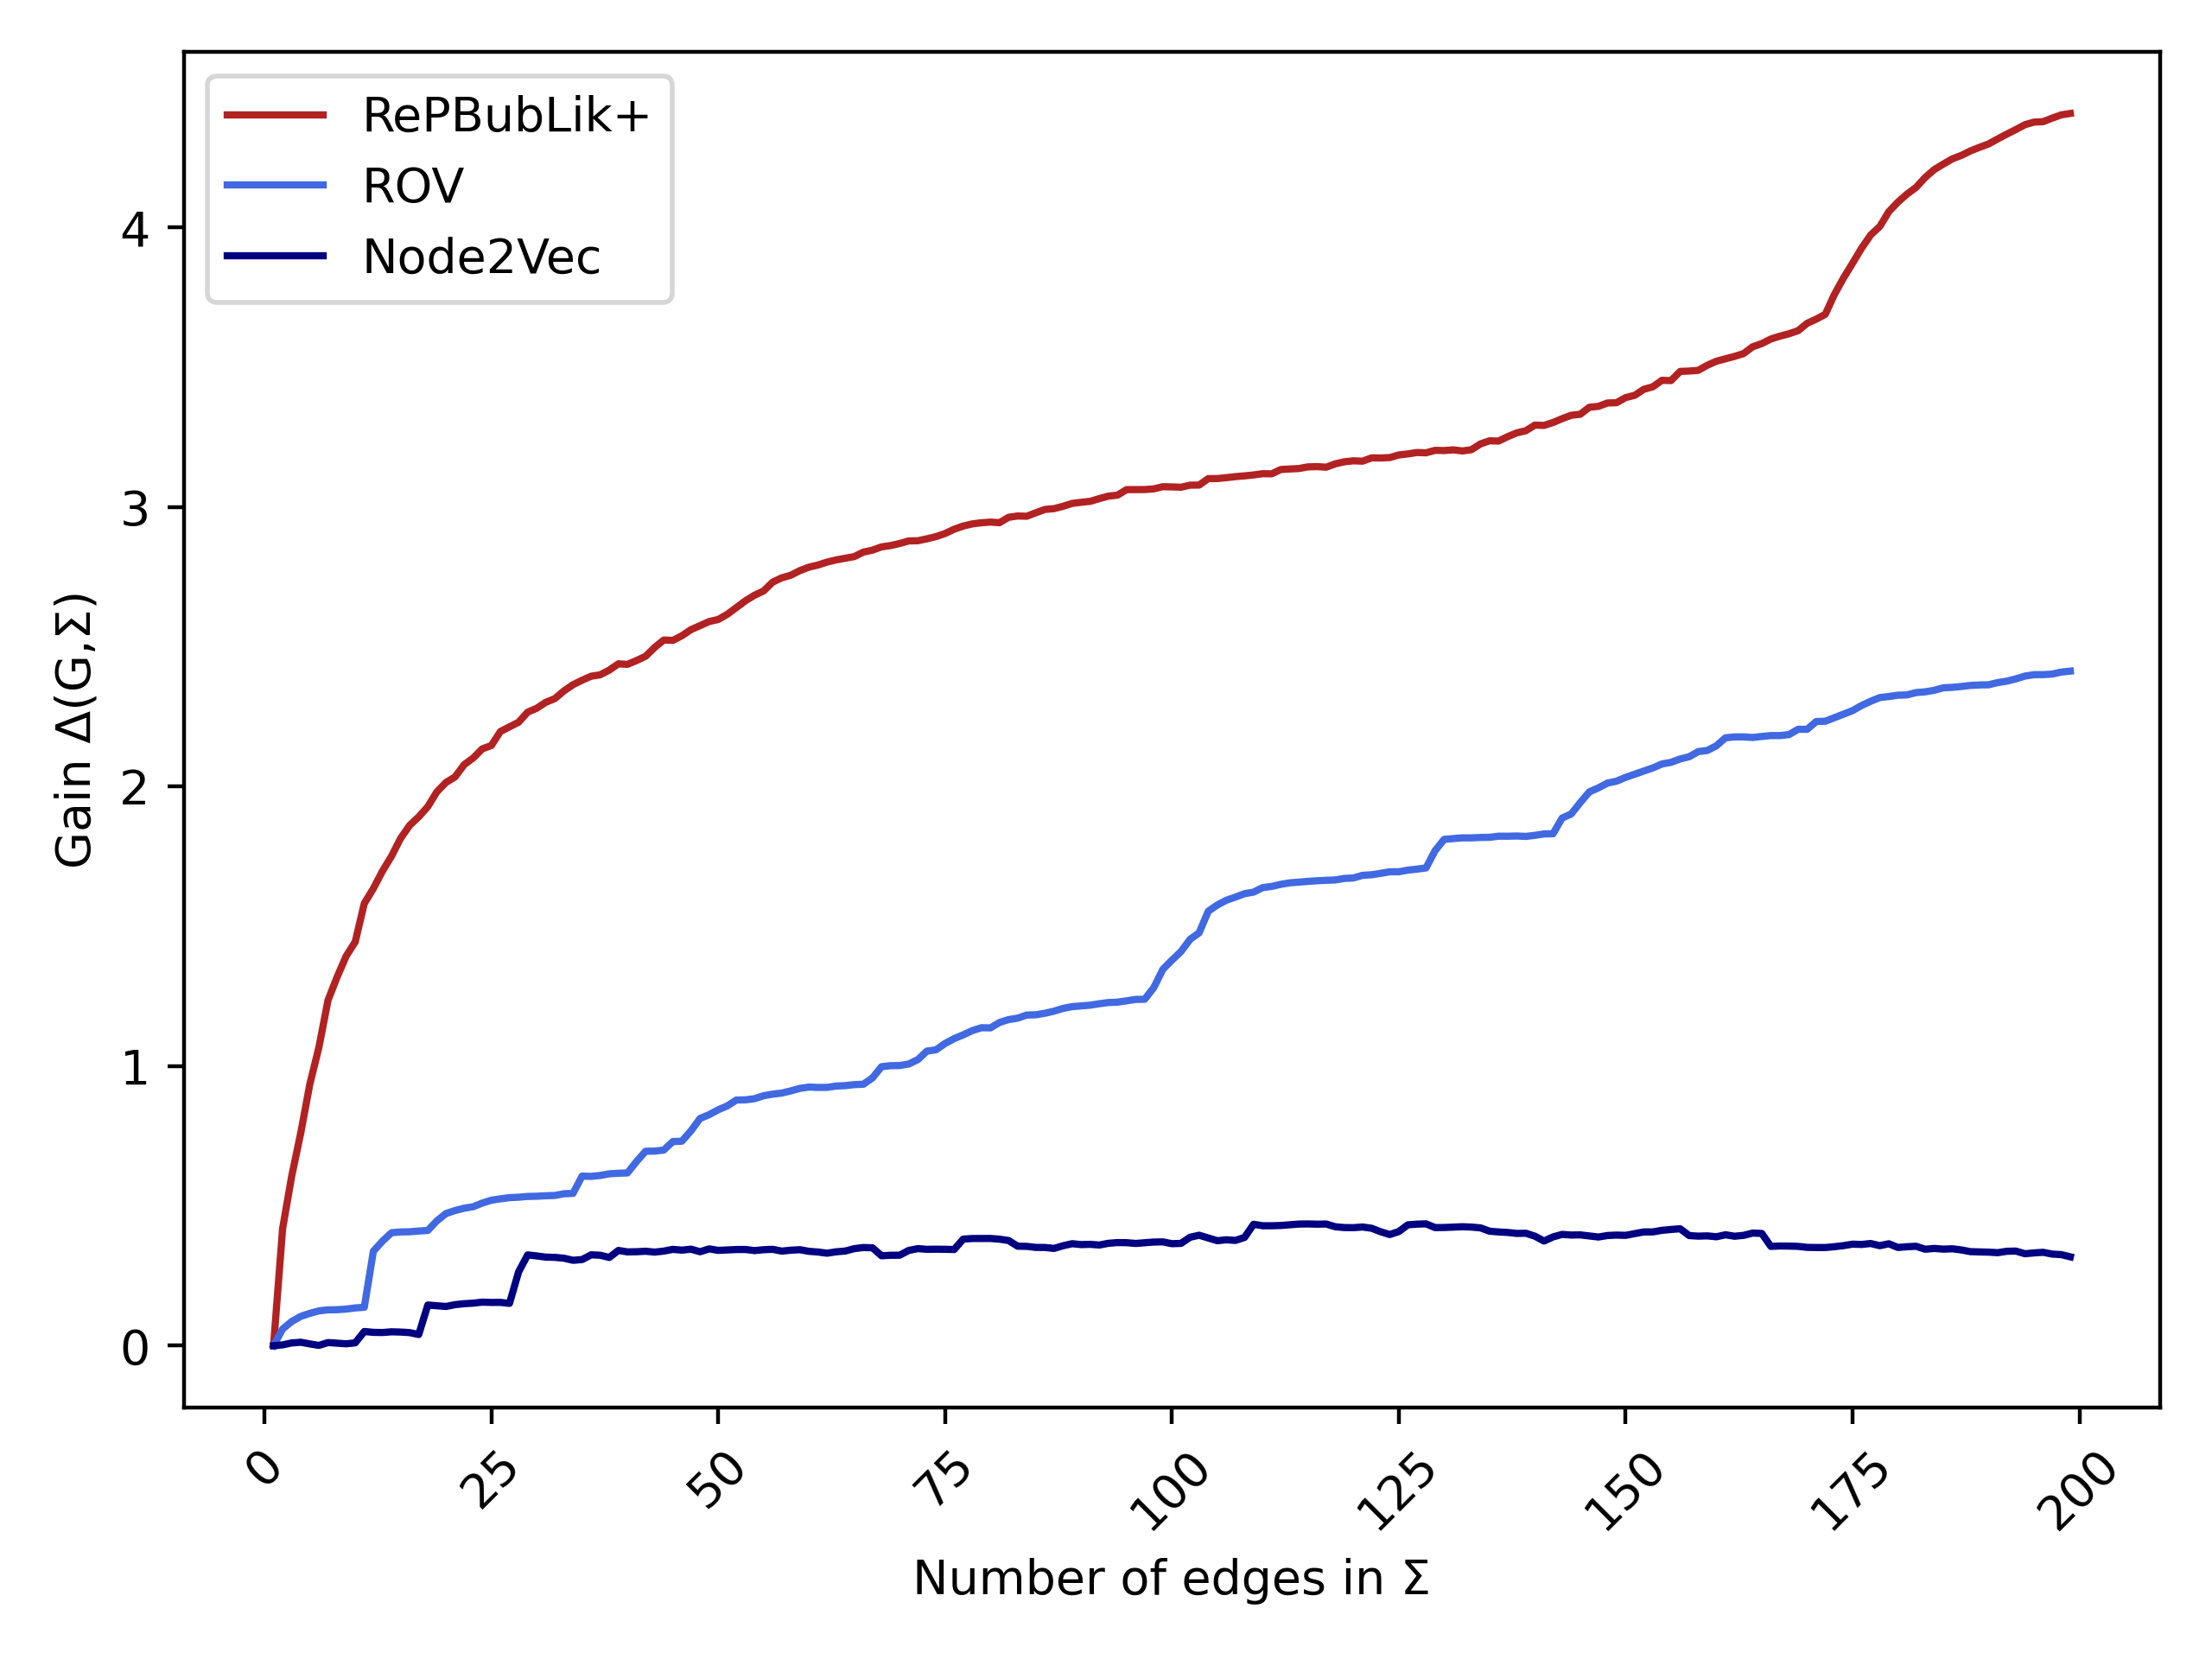
\includegraphics[width=\columnwidth]{15/polblogs_gain_15.png}
    \caption{\emph{PolBlogs} plot}\label{fig:polblogs_g_15}
\end{subfigure}
\caption{Grafici $\Delta(G,\Sigma)$ per $t=15$}
\end{figure}

Dai grafici dei guadagni, si evince che:
\begin{enumerate}
    \item RePBubLik+ è il migliore tra gli algoritmi proposti, in termini di guadagno $\Delta(G,\Sigma)$ rispetto al numero di archi in $\Sigma$.
    \item L'applicazione di RePBubLik+ a grafi di piccole dimensioni (\emph{MaTe}, \emph{MaAs}, \emph{MiHi}) porta ad un guadagno massimo maggiore rispetto a quello ottenuto mediante gli algoritmi ROV e Node2Vec (es. (\emph{MaAs}) ${\Delta_{R+}\over{\Delta_{ROV}}}=2.93$, ${\Delta_{R+}\over{\Delta_{Node2Vec}}}=2.56$ per $k=200,t=10$).
    \item L'applicazione di RePBubLik+ a grafi di medie dimensioni (\emph{PolBlogs}) porta ad un guadagno massimo maggiore rispetto a quello ottenuto mediante gli algoritmi ROV e Node2Vec (es. (\emph{PolBlogs}) ${\Delta_{R+}\over{\Delta_{ROV}}}=2.34$, ${\Delta_{R+}\over{\Delta_{Node2Vec}}}=18.67$ per  $k=200,t=10$).
    \item RePBubLik+ risulta essere il miglior algoritmo in quanto per un numero ridotto di archi riporta un notevole guadagno: nei grafici sovrastanti, la curva dell'algoritmo RePBubLik+ cresce molto rapidamente per valori piccoli di $k$, raggiungendo una plateau per un certo valore di $\Delta(G,\Sigma)$.
            Questo, dal punto di vista pratico, è molto interessante perchè permette con pochi archi aggiuntivi di ridurre notevolmente la polarizzazione in grafi simili a quelli presi in esame (es. (\emph{MaTe}) ${\Delta_{R+}\over{\Delta_{ROV}}}=7.45$, ${\Delta_{R+}\over{\Delta_{Node2Vec}}}=3.35$ per $k=50,t=10$).
    \item Le considerazioni fatte nei punti precedenti sono generalmente valide, per qualsiasi valore di $t$ e qualsiasi grafo. Valutando i guadagni dei grafi anche in termini di RW massimo, si può notare che per valori di $t$ maggiori, RePBubLik+ raggiunge il plateau con un numero inferiore d'archi (es. (\emph{MaTe}) $\Delta_{R+}=2$ per $k=50, t=5$,  $\Delta_{R+}=6.75$ per $k=50,t=10$, $\Delta_{R+}=11.5$ per $k=50,t=15$).
\end{enumerate}
\subsection{Bias strutturale $\rho(G)$}
L'ultima metrica che viene anlizzata è il il bias $\rho(G)$ (\ref{REP:bias}) in relazione al numero 
degli archi aggiunti al grafo $G$. Lo studio di questa misura è interessante, in quanto permette di valutare il cambiamento della polarizzazione del grafo $G$.
\\
Di seguito i bias per ciascun grafo e per ciascun valore di $t$.

\begin{figure}[!h]
    \centering
\begin{subfigure}[b]{0.4\textwidth}
    \centering
    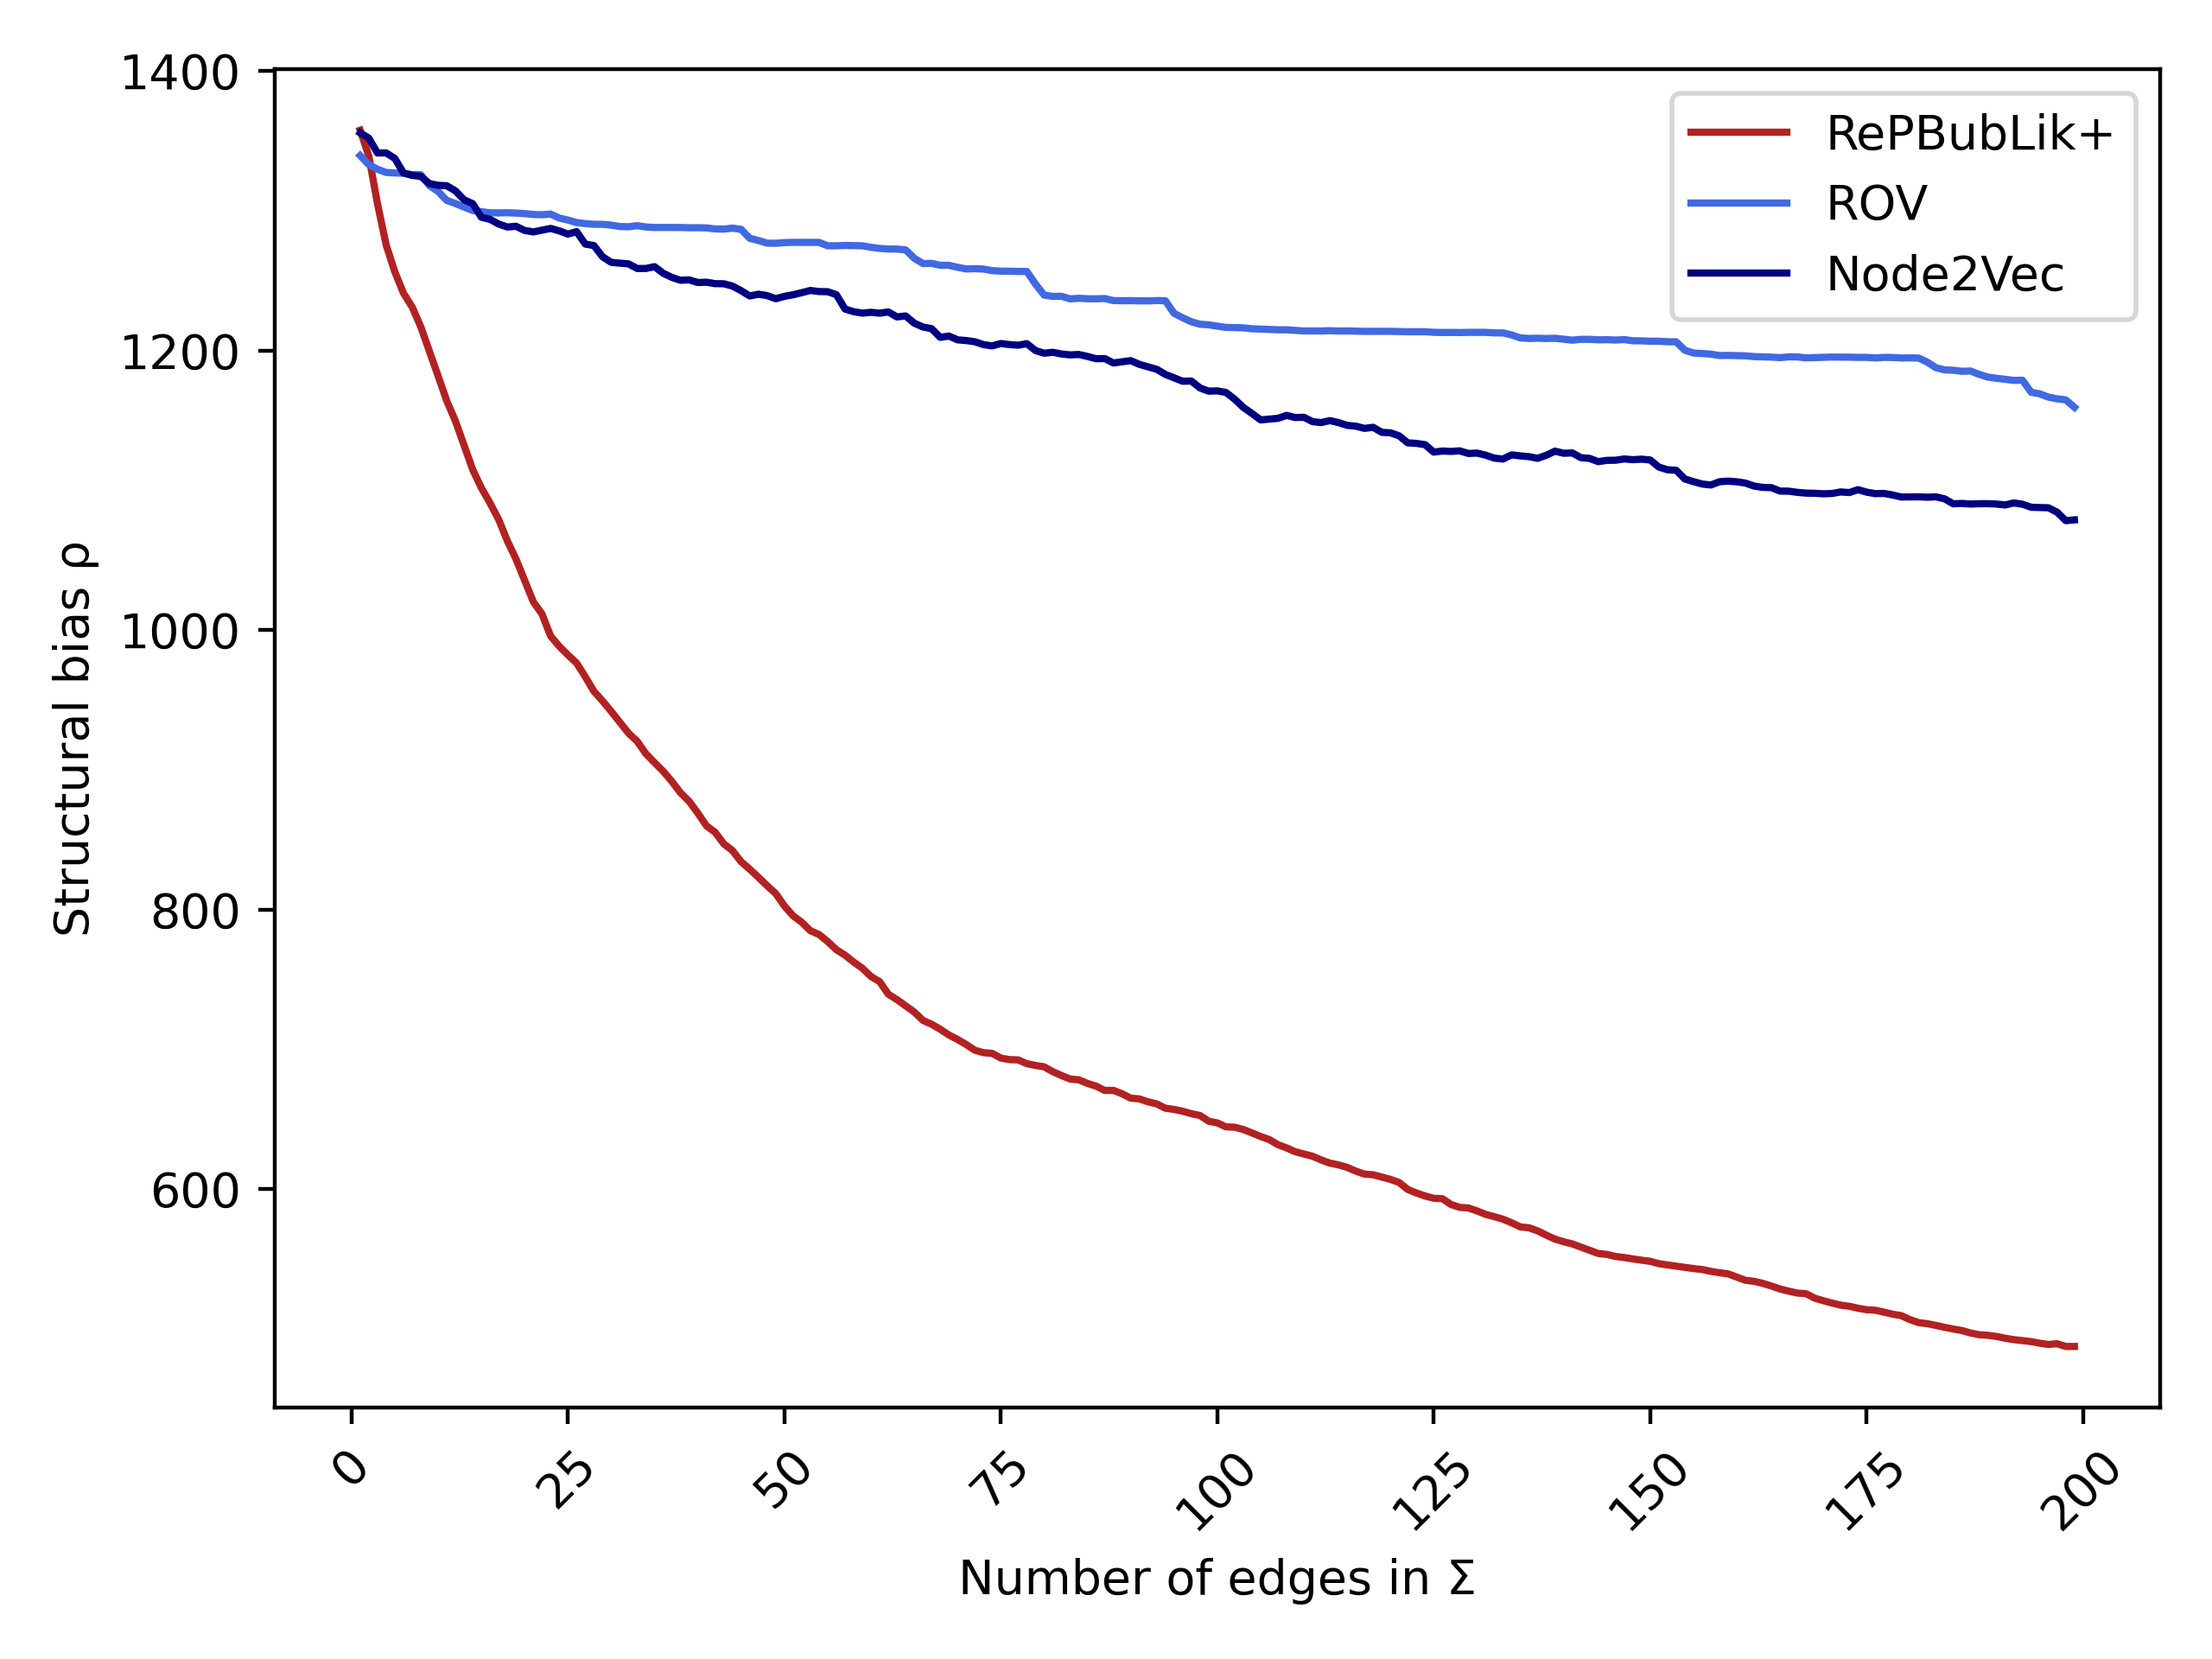
\includegraphics[width=\columnwidth]{5/math_tech_bias_5.png}
    \caption{\emph{MaTe} plot}\label{fig:mate_b_5}
\end{subfigure}
\hspace{0.1\columnwidth}
\begin{subfigure}[b]{0.4\textwidth}
    \centering
    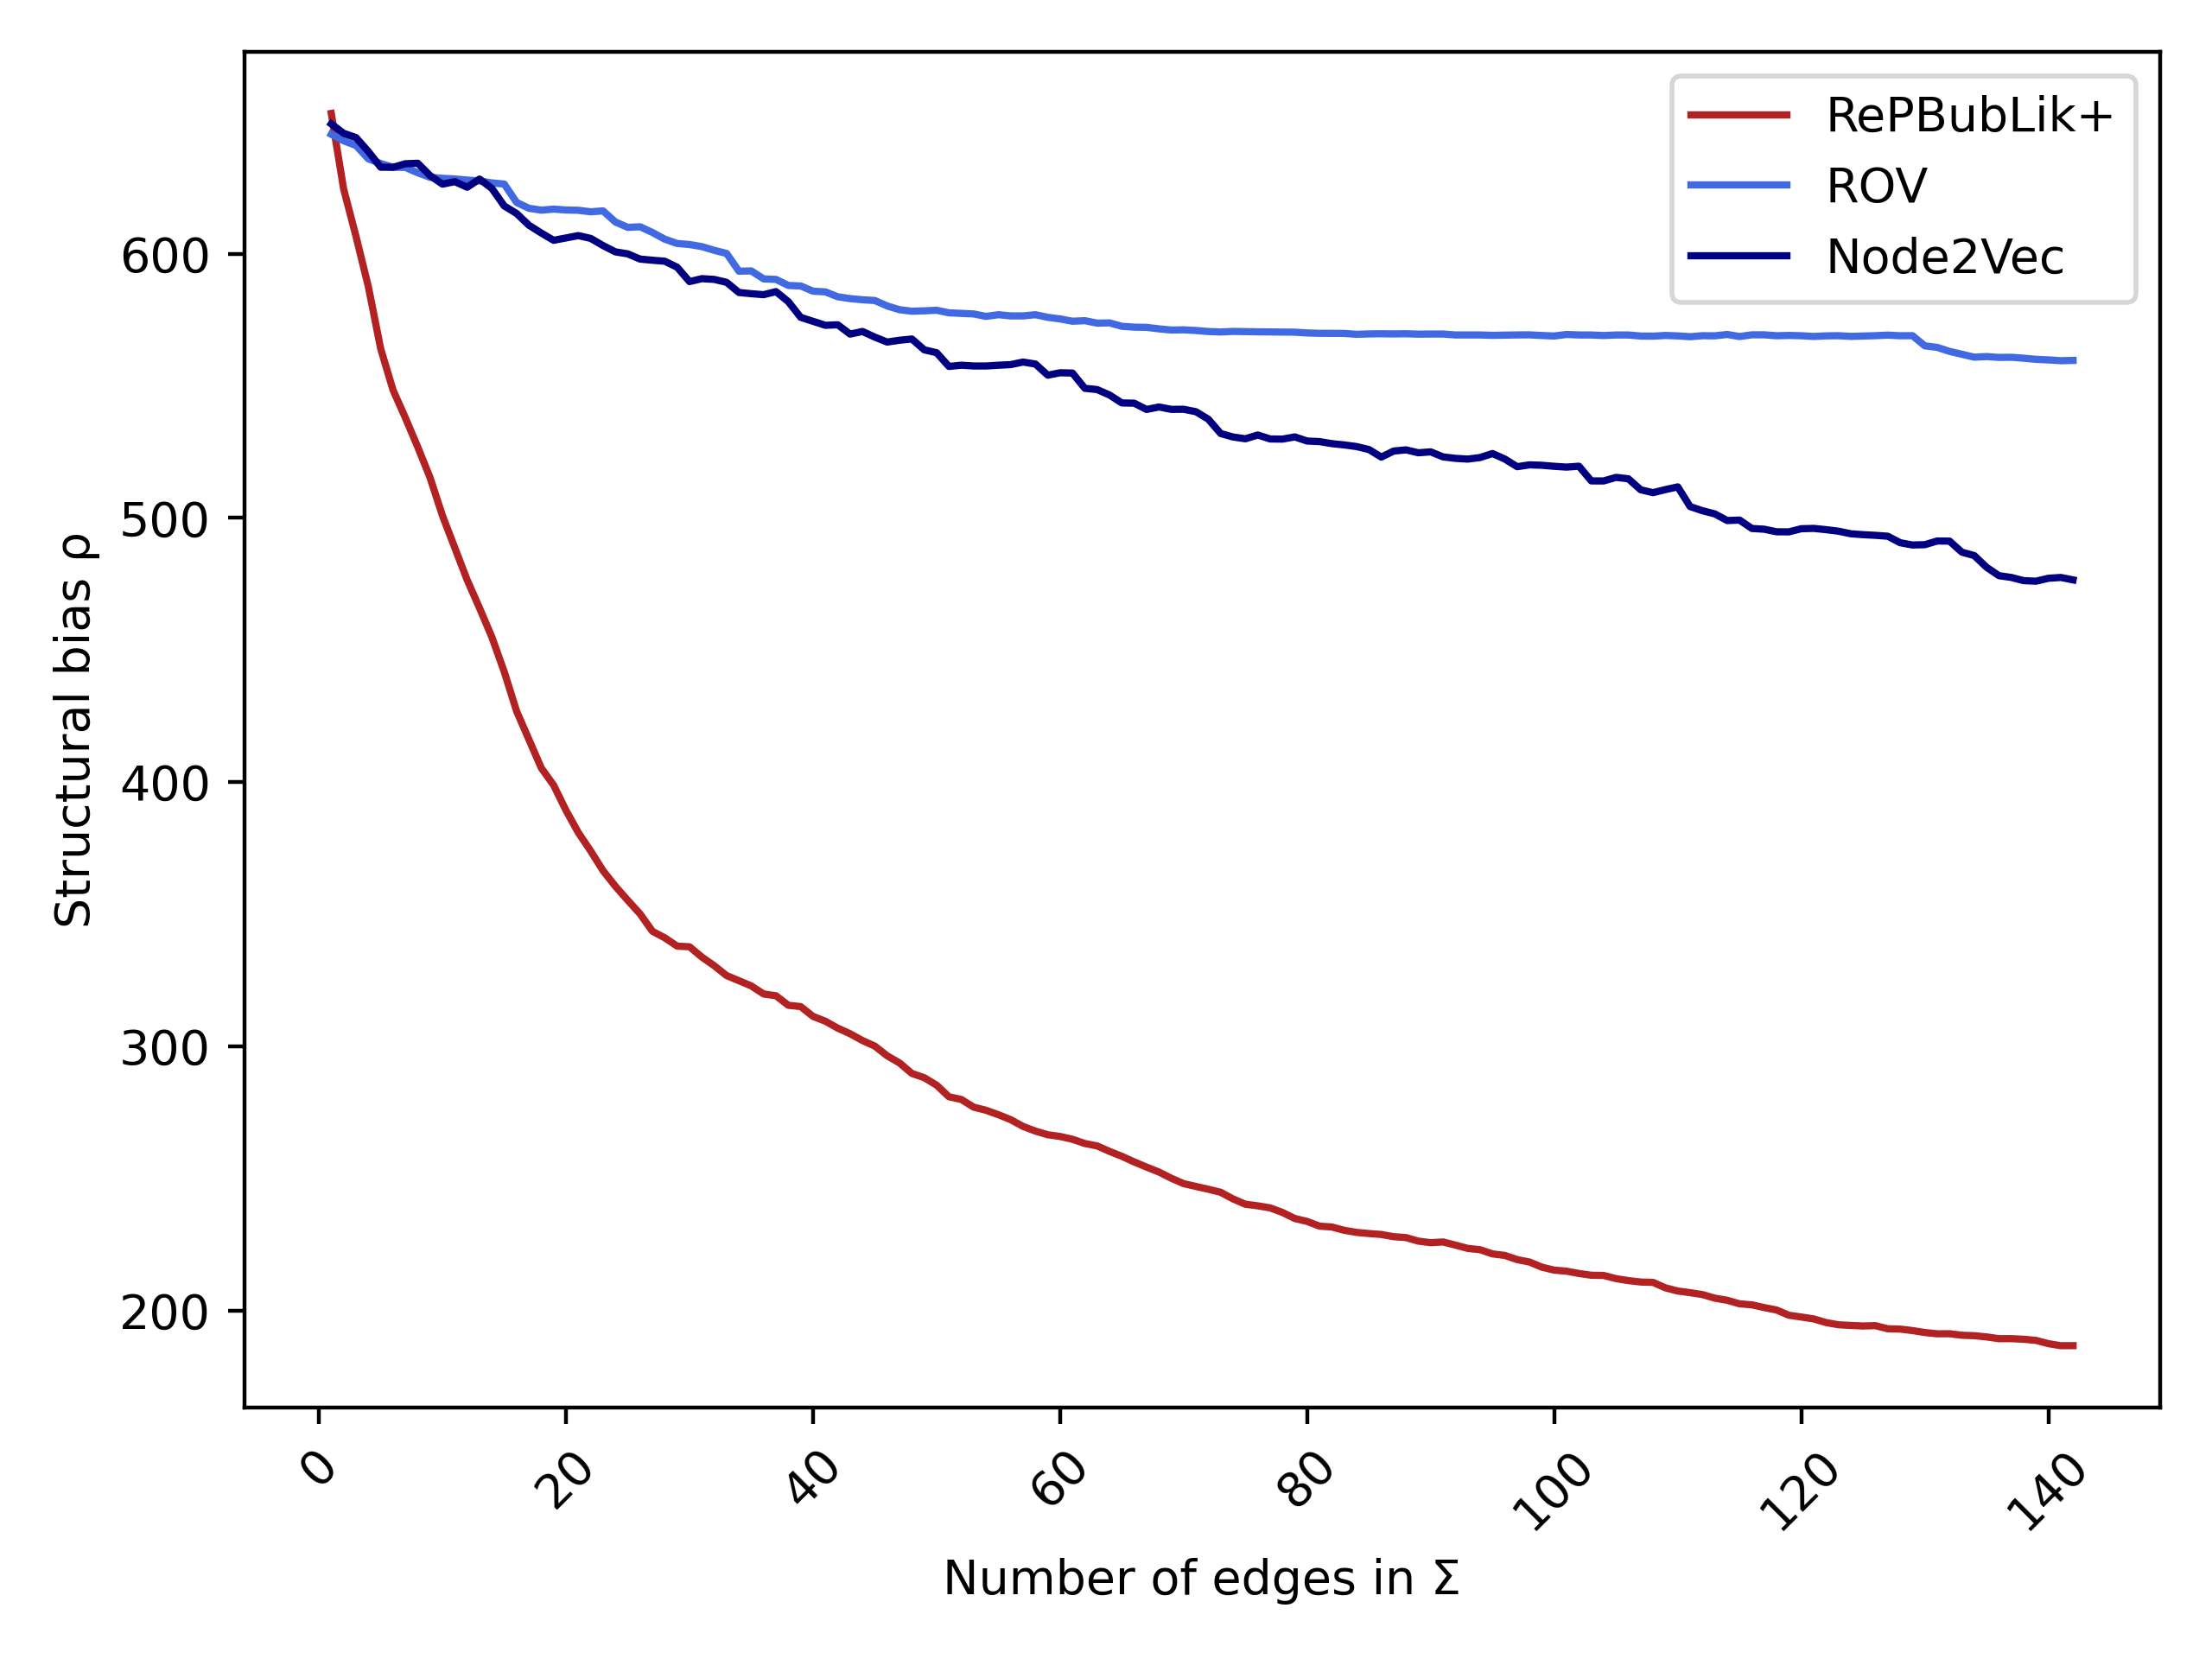
\includegraphics[width=\columnwidth]{5/tech_mil_bias_5.png}
    \caption{\emph{MiHi} plot}\label{fig:mihi_b_5}
\end{subfigure}

\begin{subfigure}[b]{0.4\textwidth}
    \centering
    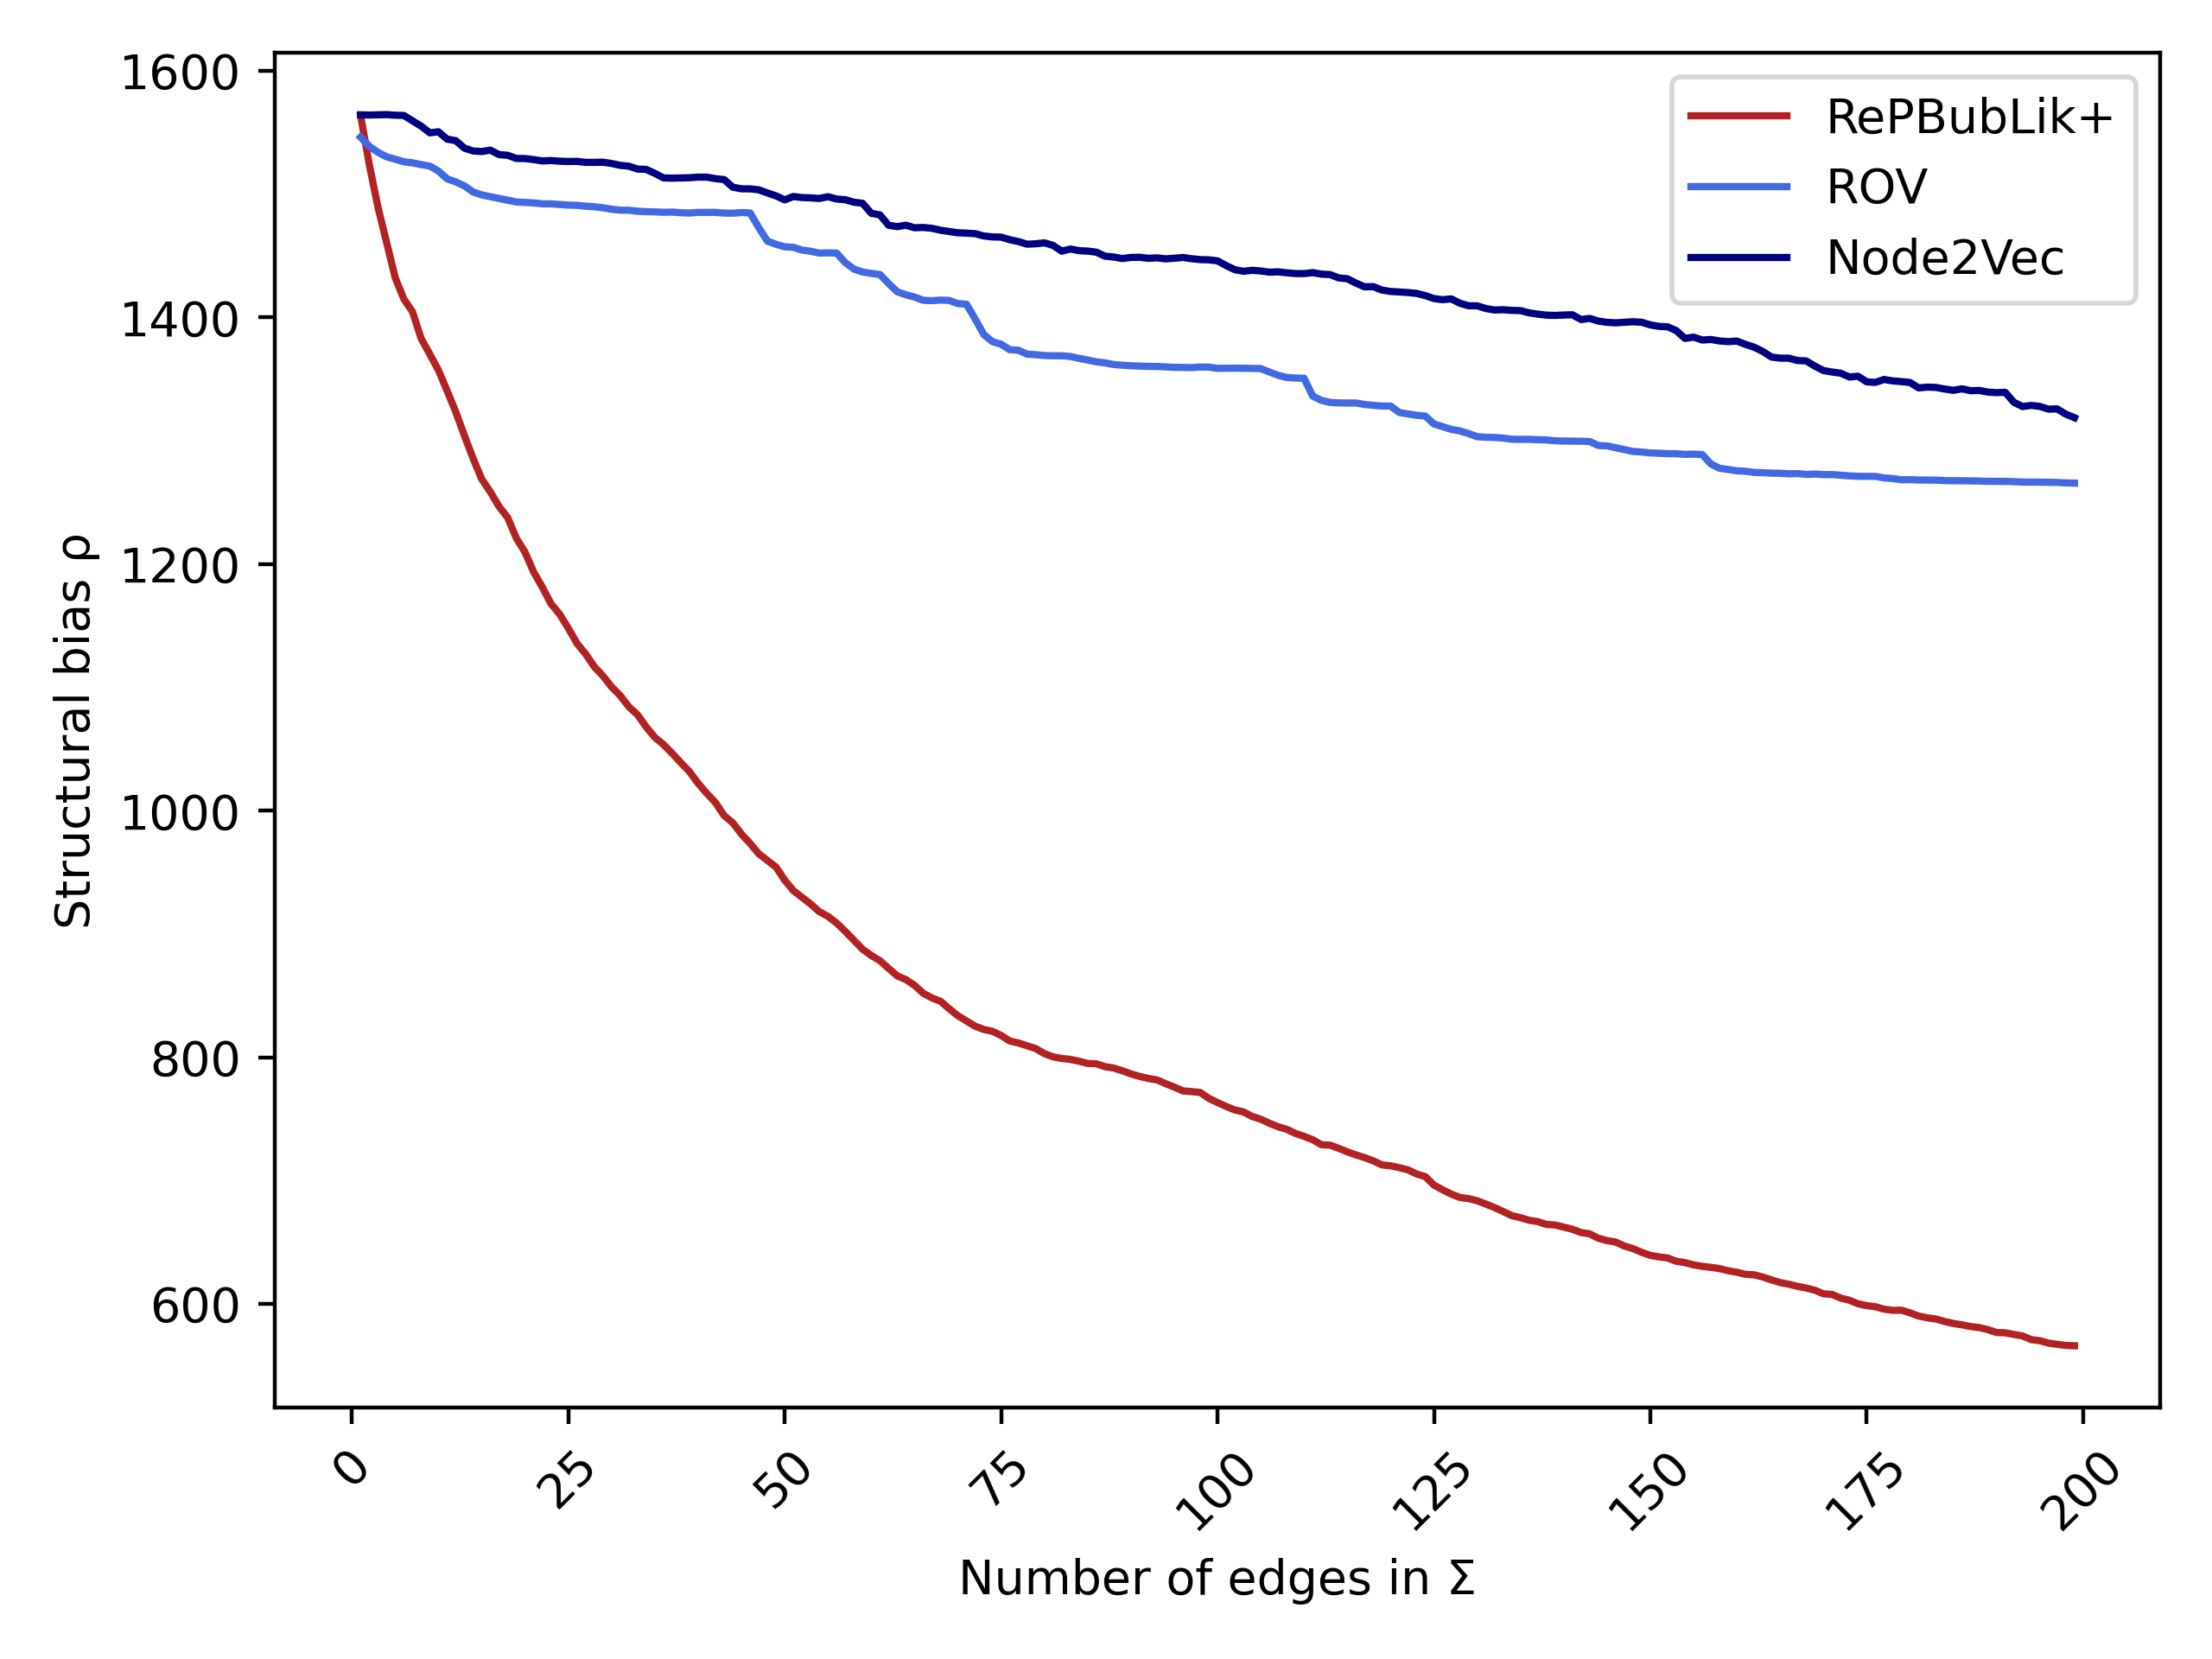
\includegraphics[width=\columnwidth]{5/math_ast_bias_5.png}
    \caption{\emph{MaA}s plot}\label{fig:maas_b_5}
\end{subfigure}
\hspace{0.1\columnwidth}
\begin{subfigure}[b]{0.4\textwidth}
    \centering
    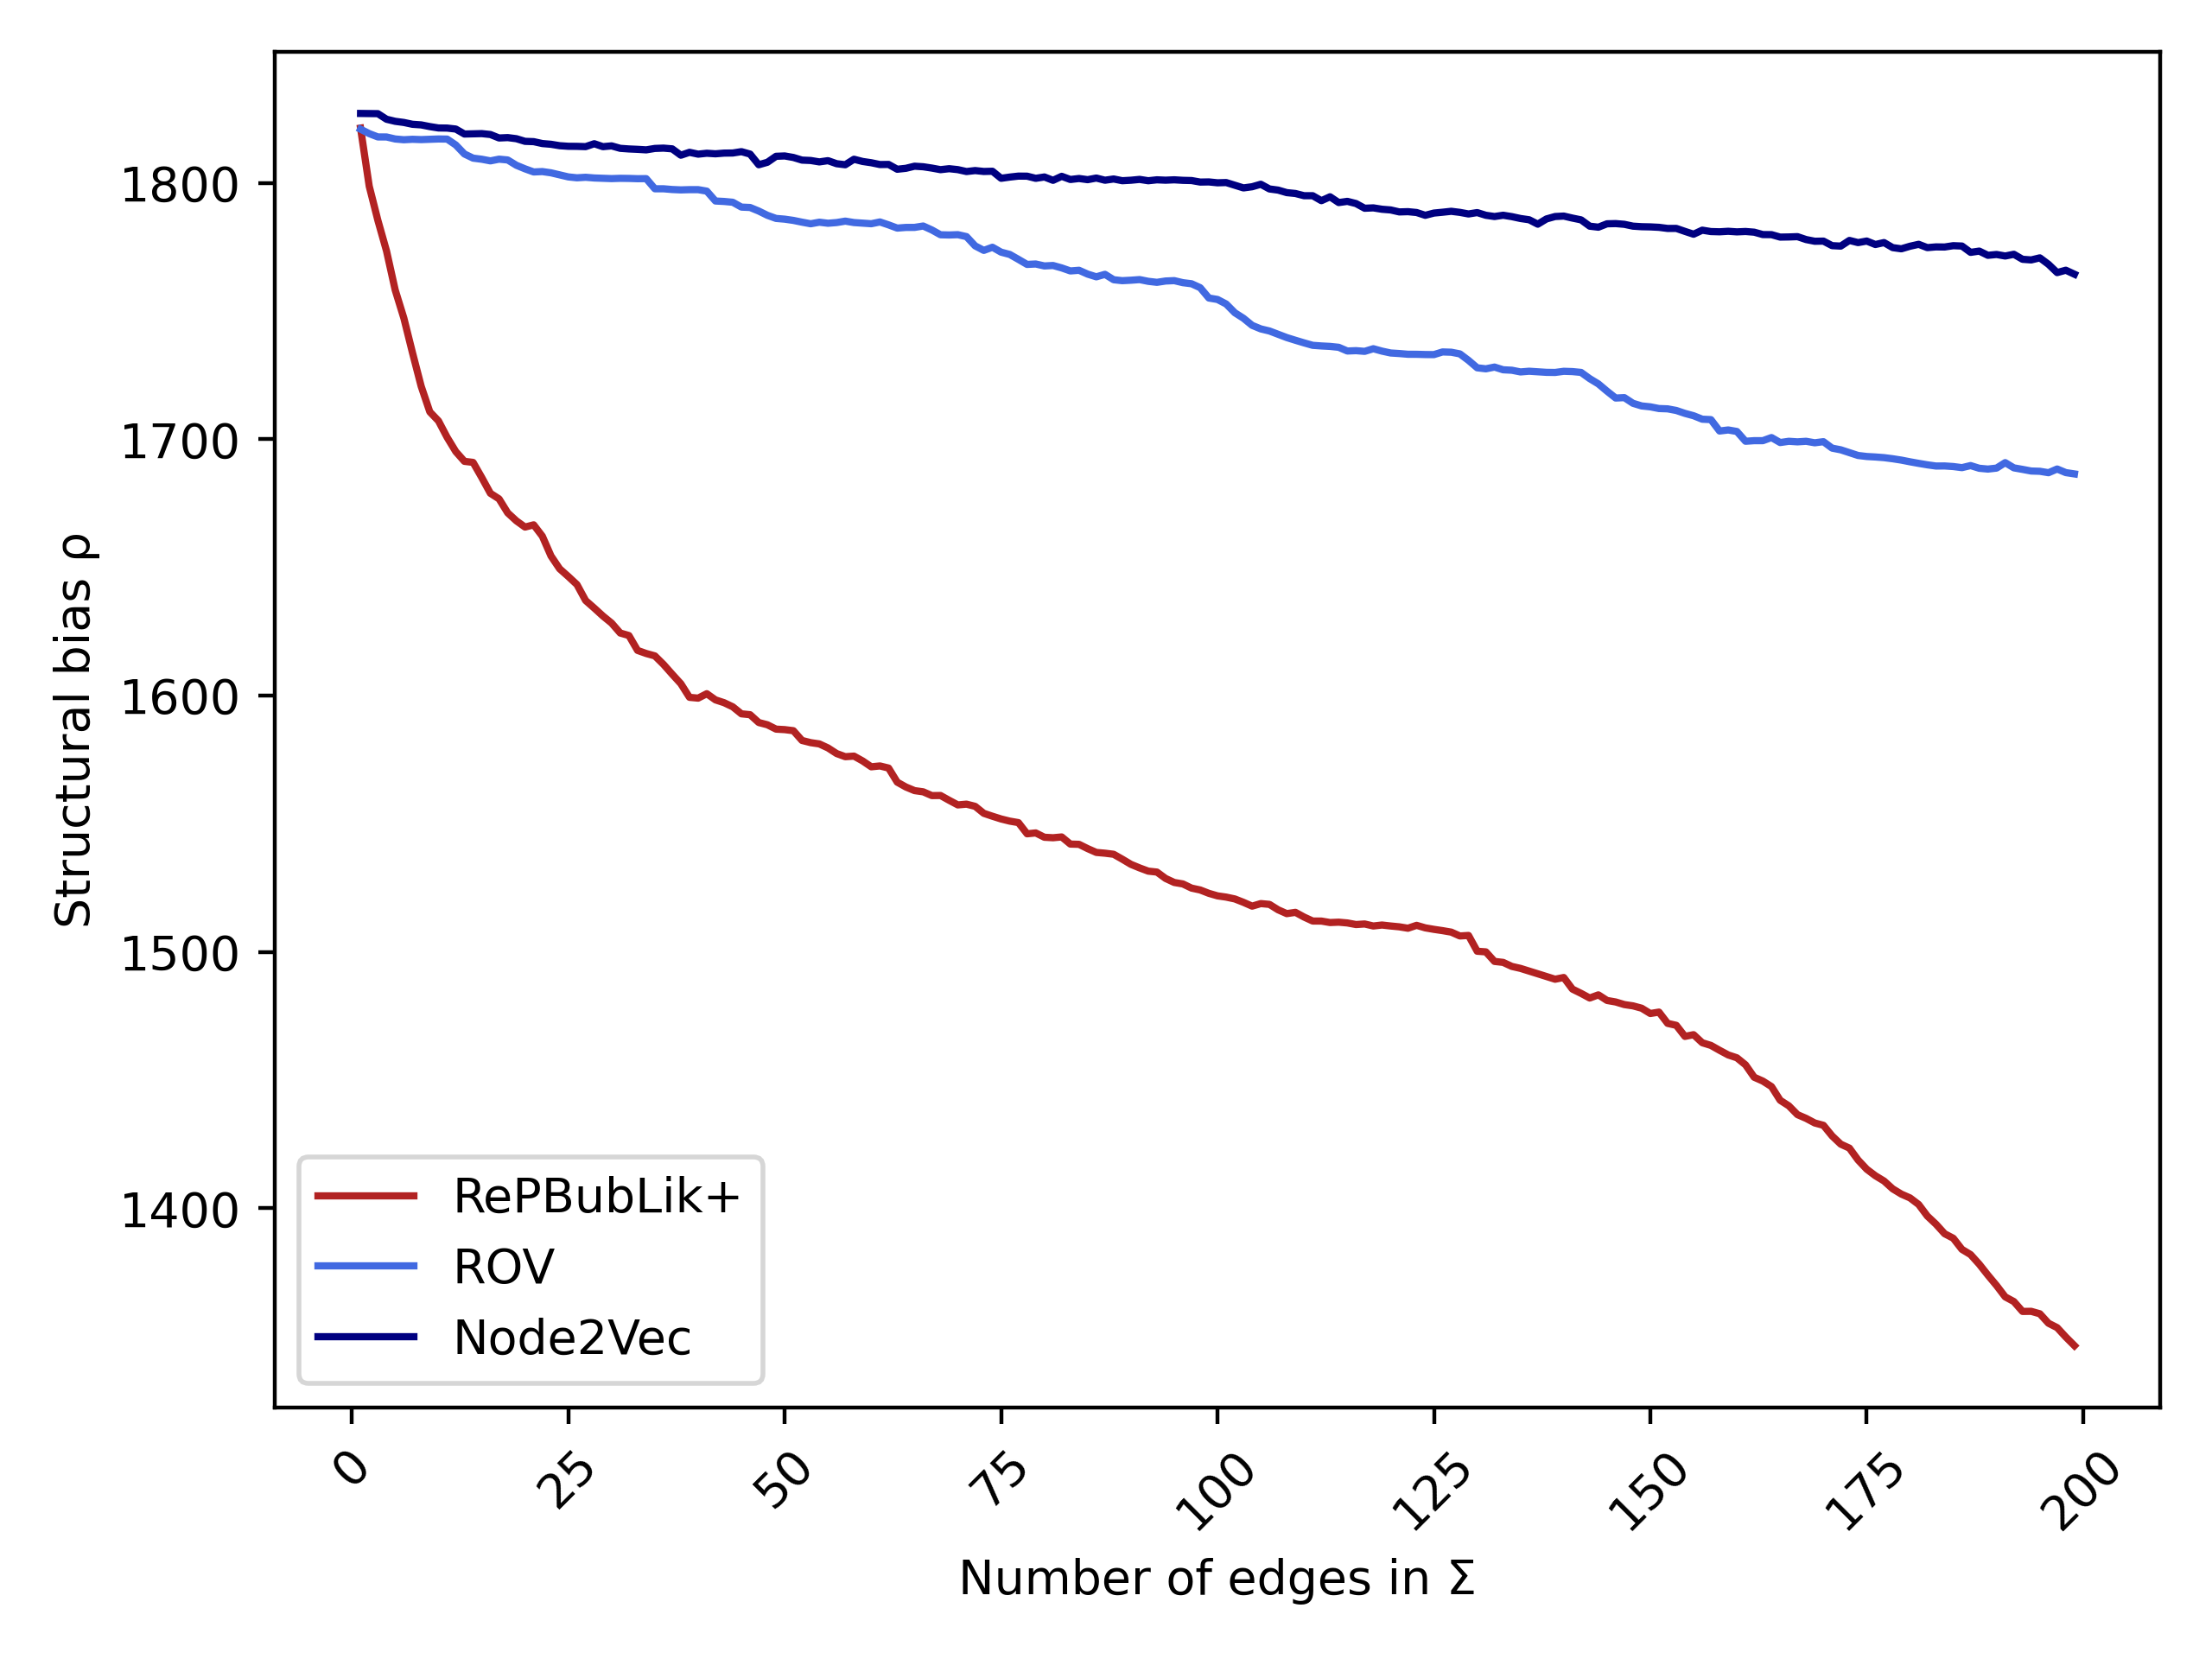
\includegraphics[width=\columnwidth]{5/polblogs_bias_5.png}
    \caption{\emph{PolBlogs} plot}\label{fig:polblogs_b_5}
\end{subfigure}
\caption{Grafici $\rho(G)$ per $t=5$}
\end{figure}
\begin{figure}[!h]
    \centering
\begin{subfigure}[b]{0.4\textwidth}
    \centering
    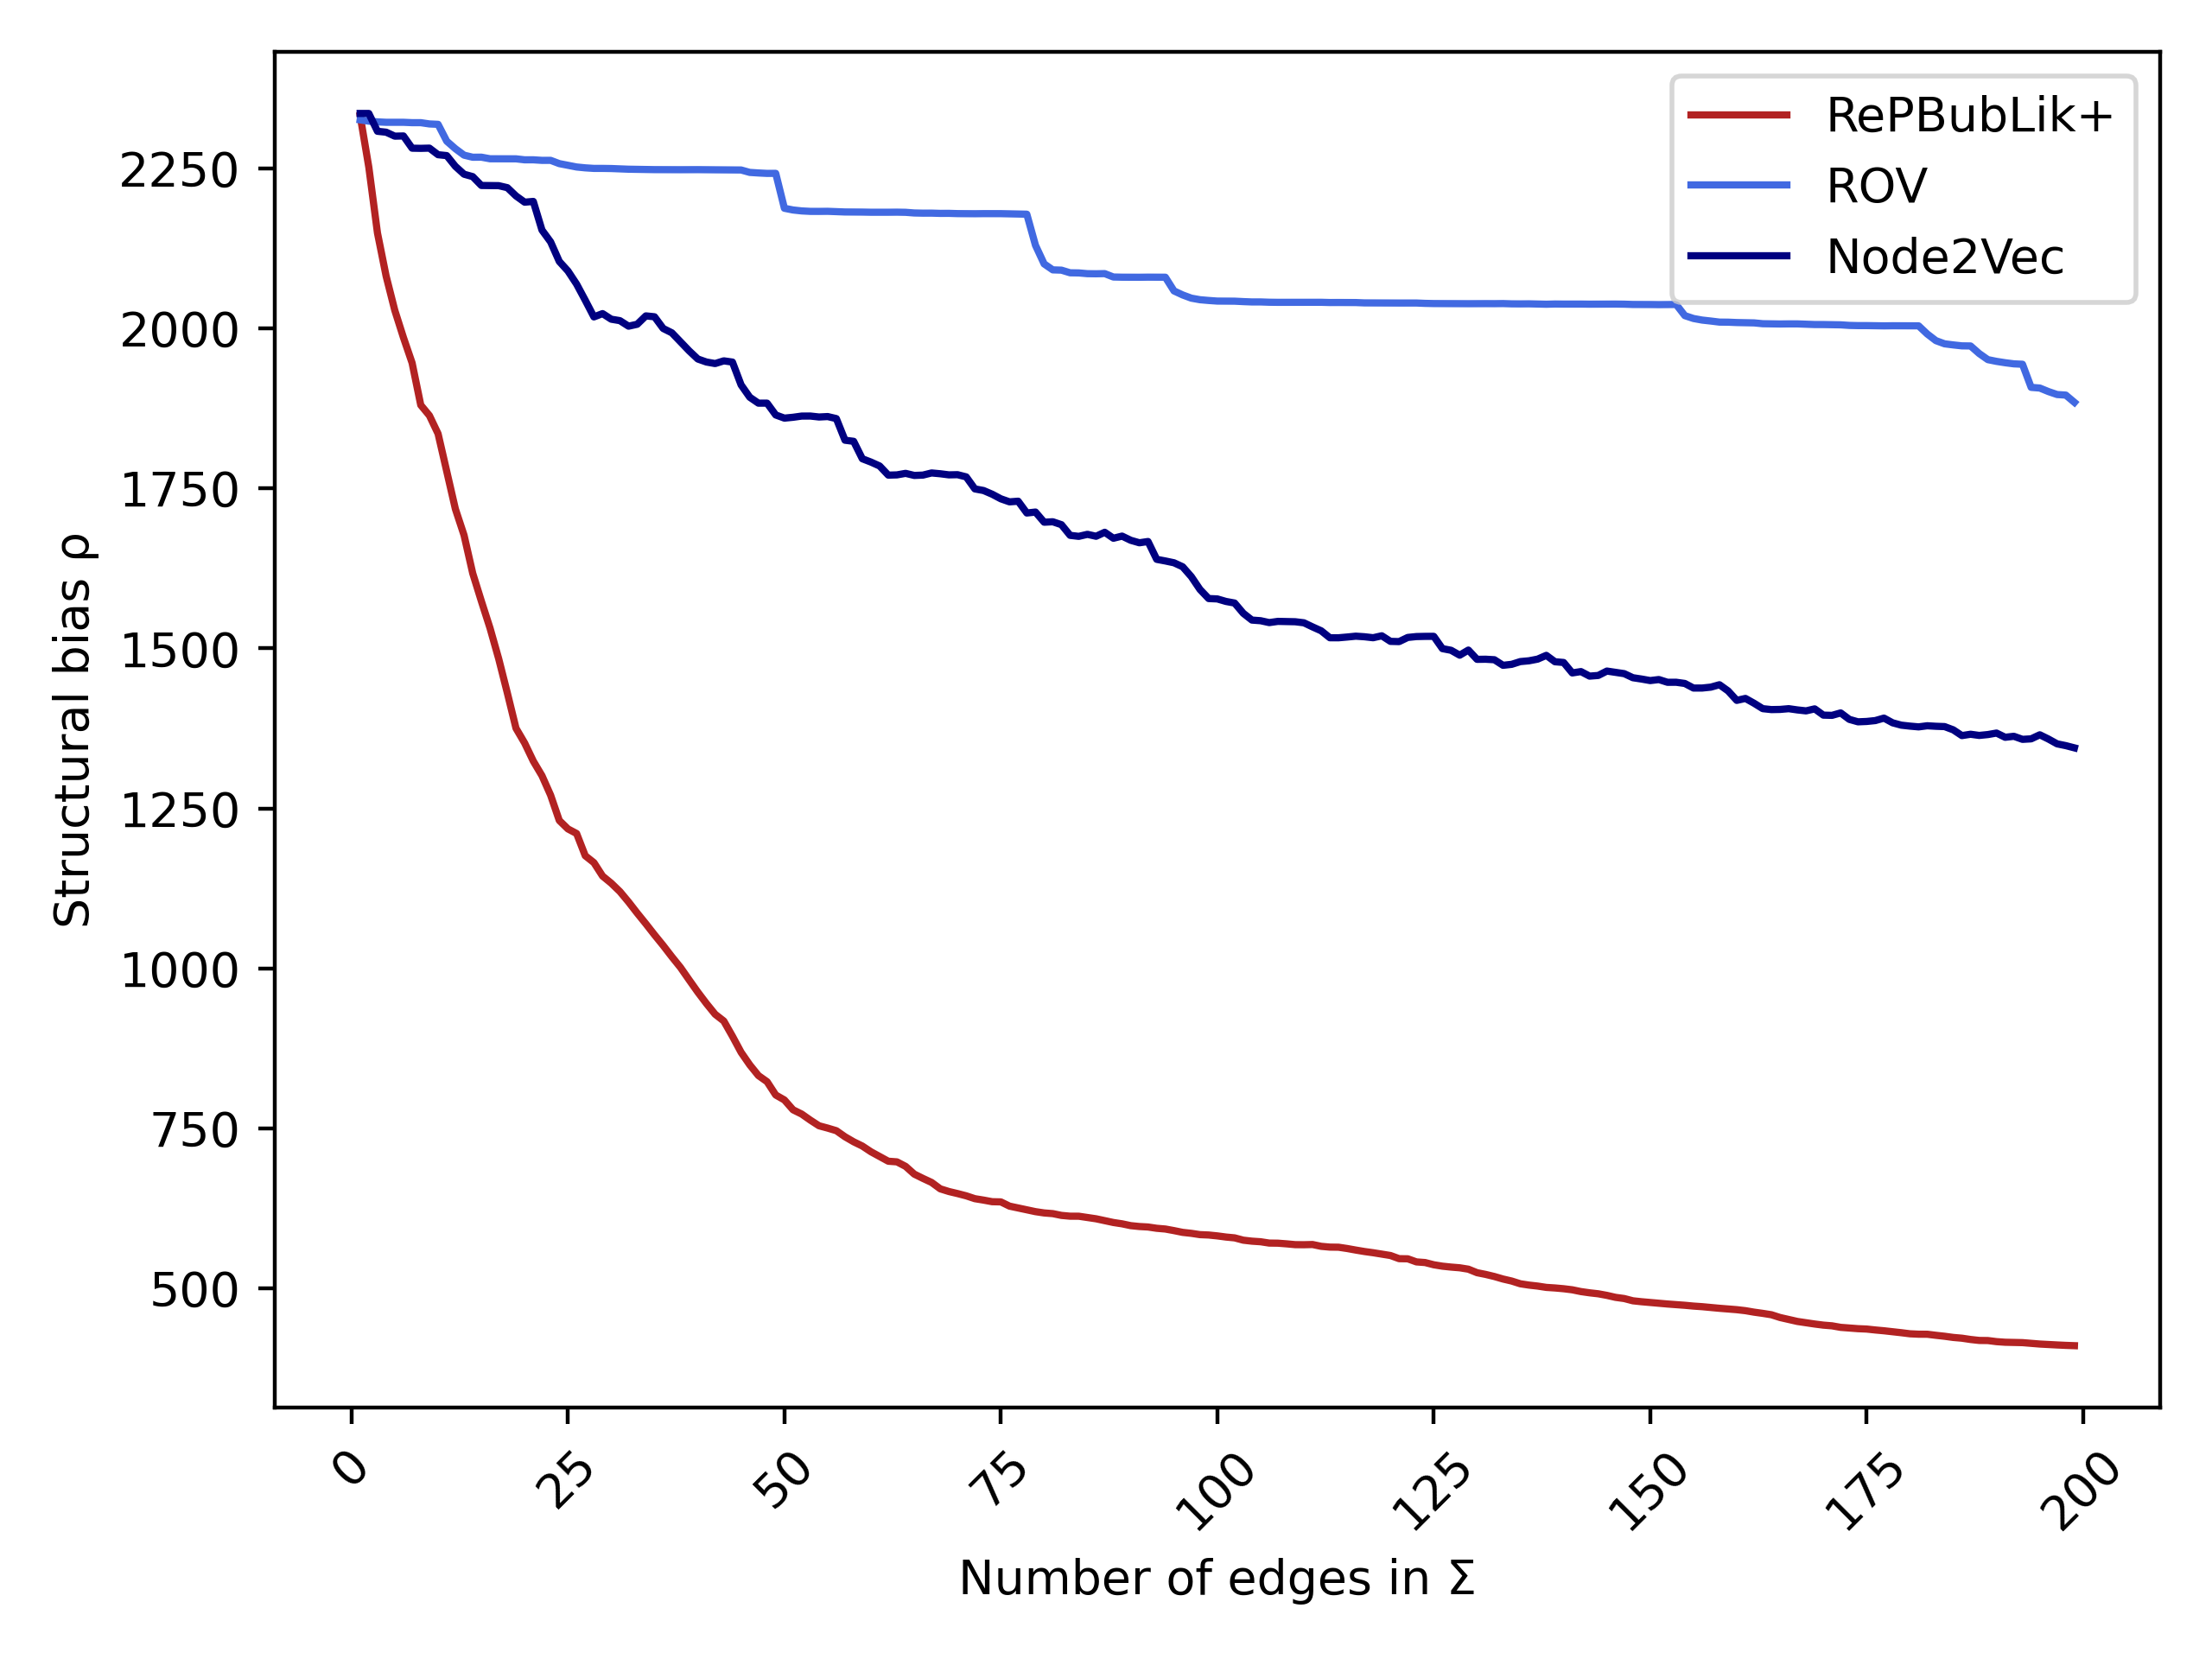
\includegraphics[width=\columnwidth]{10/math_tech_bias_10.png}
    \caption{\emph{MaTe} plot}\label{fig:mate_b_10}
\end{subfigure}
\hspace{0.1\columnwidth}
\begin{subfigure}[b]{0.4\textwidth}
    \centering
    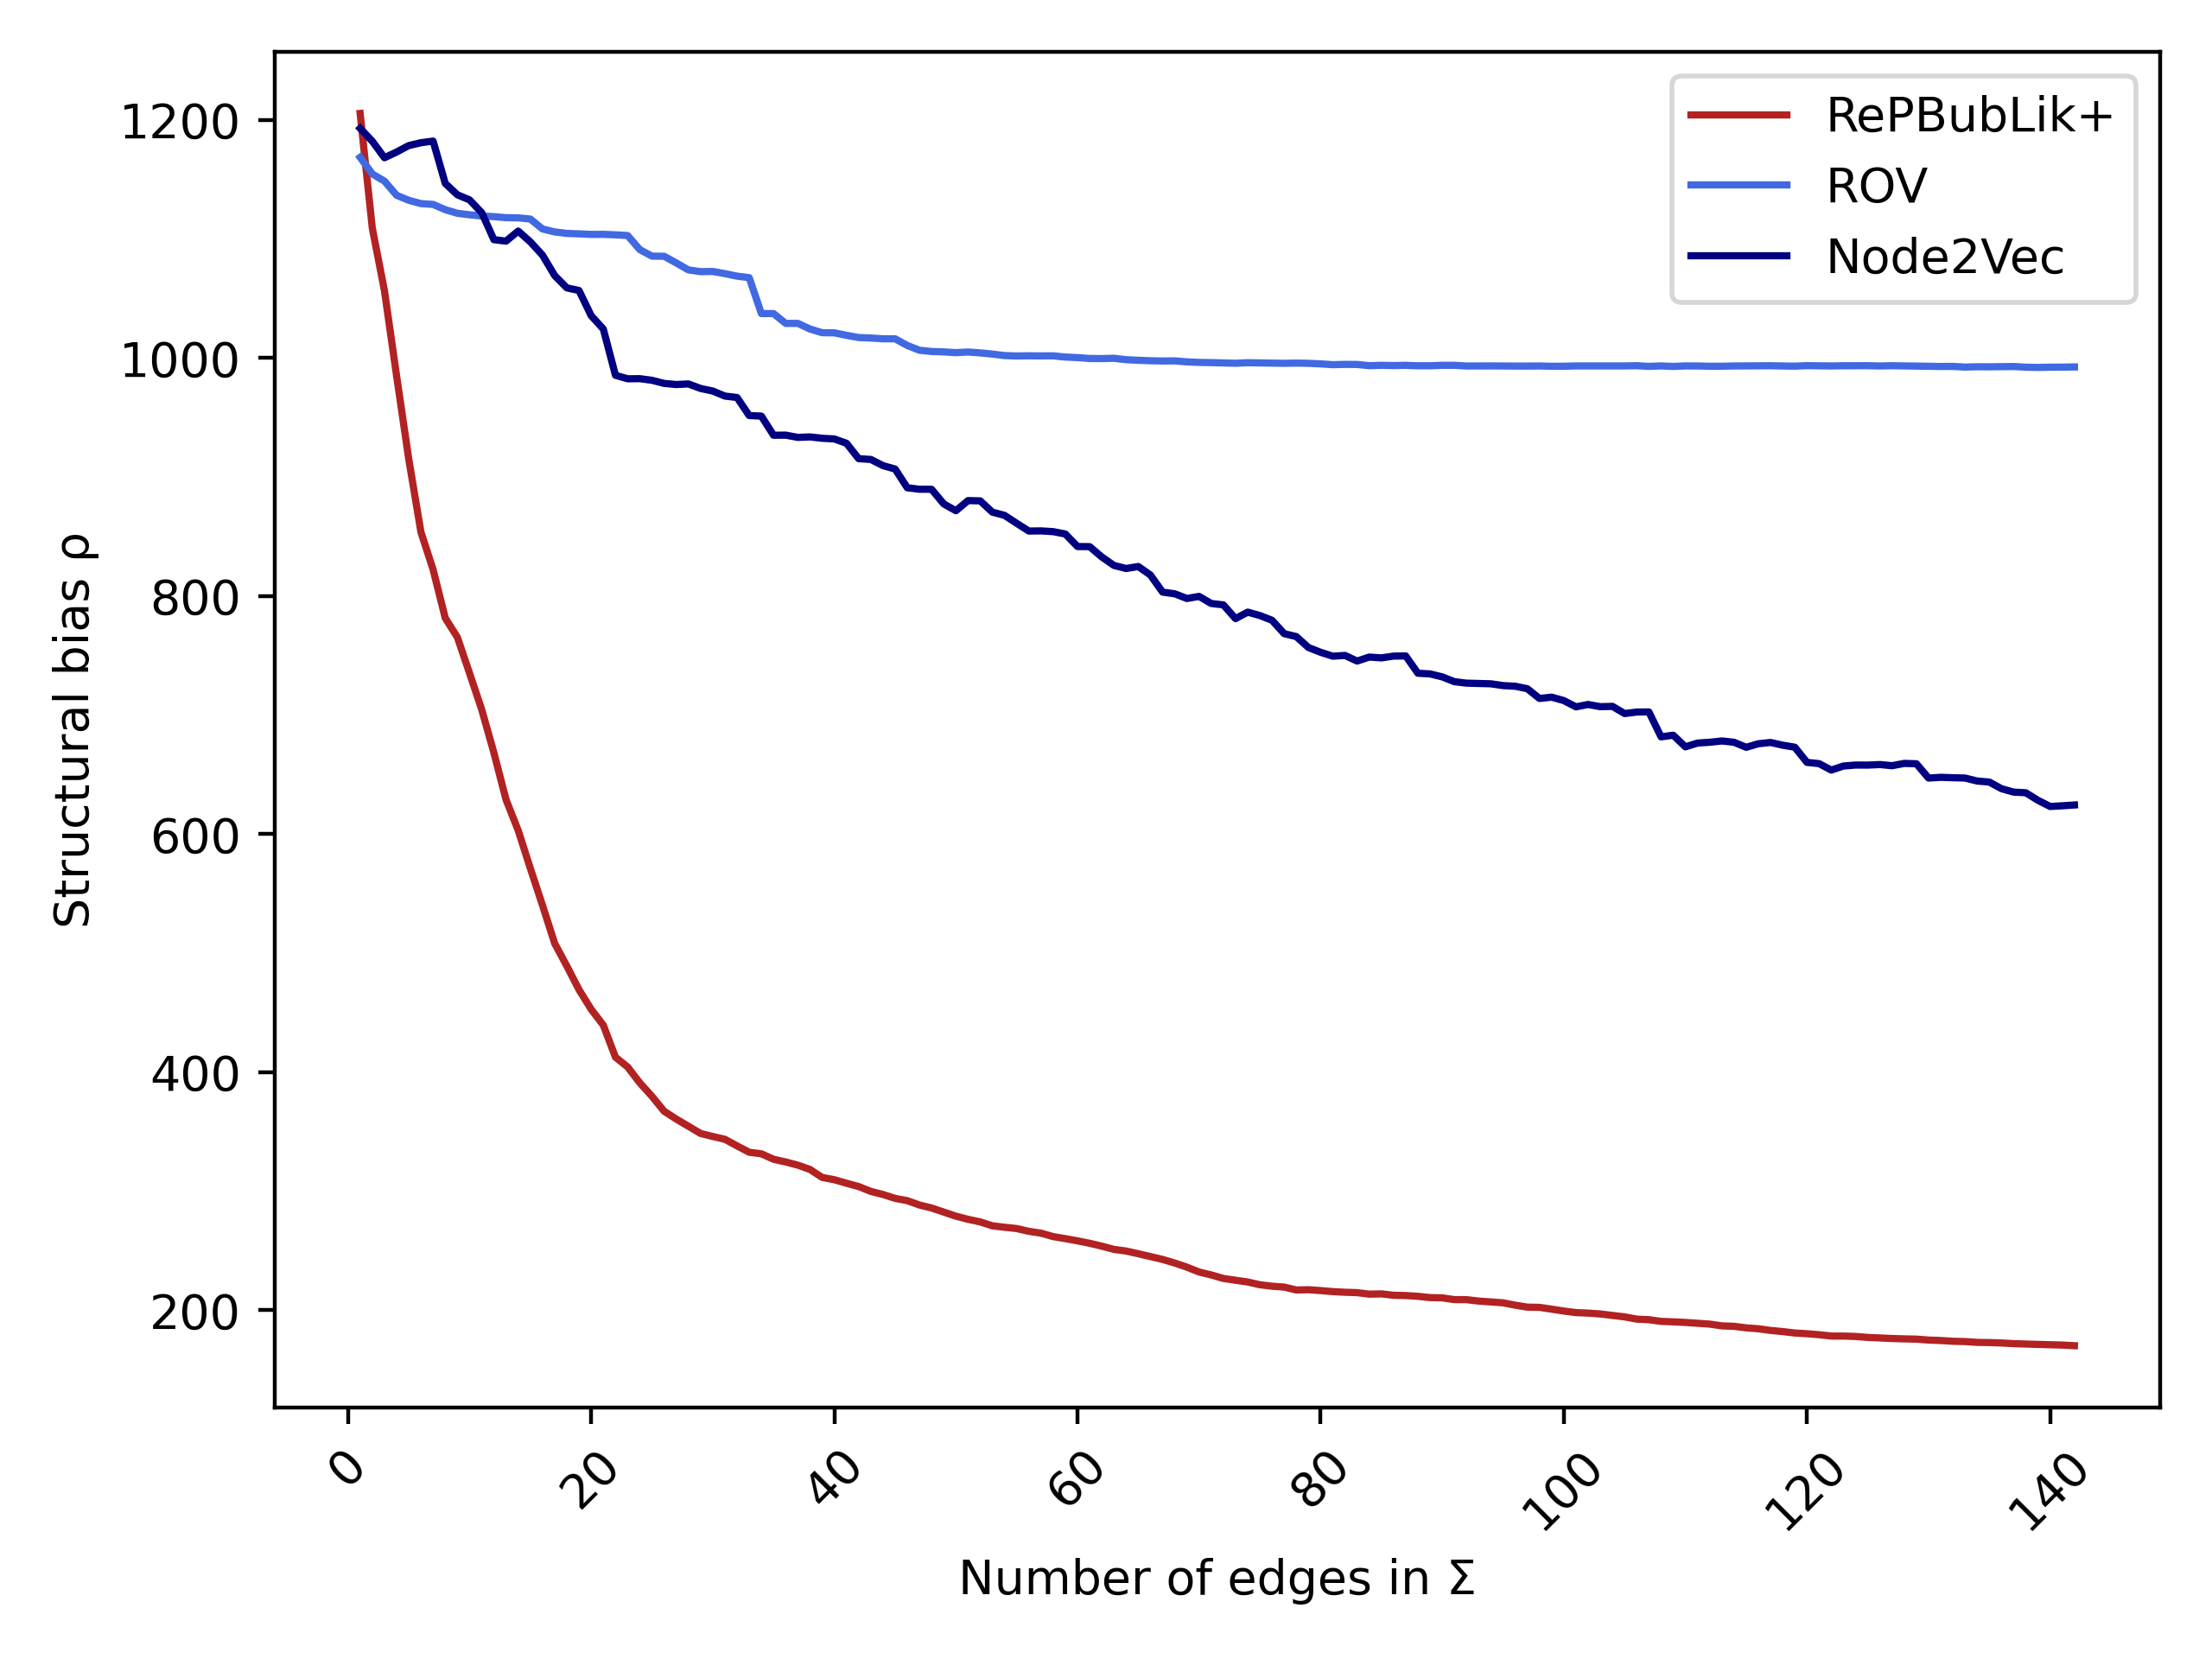
\includegraphics[width=\columnwidth]{10/tech_mil_bias_10.png}
    \caption{\emph{MiHi} plot}\label{fig:mihi_b_10}
\end{subfigure}
\end{figure}
\begin{figure}
    \ContinuedFloat
    \centering
\begin{subfigure}[b]{0.4\textwidth}
    \centering
    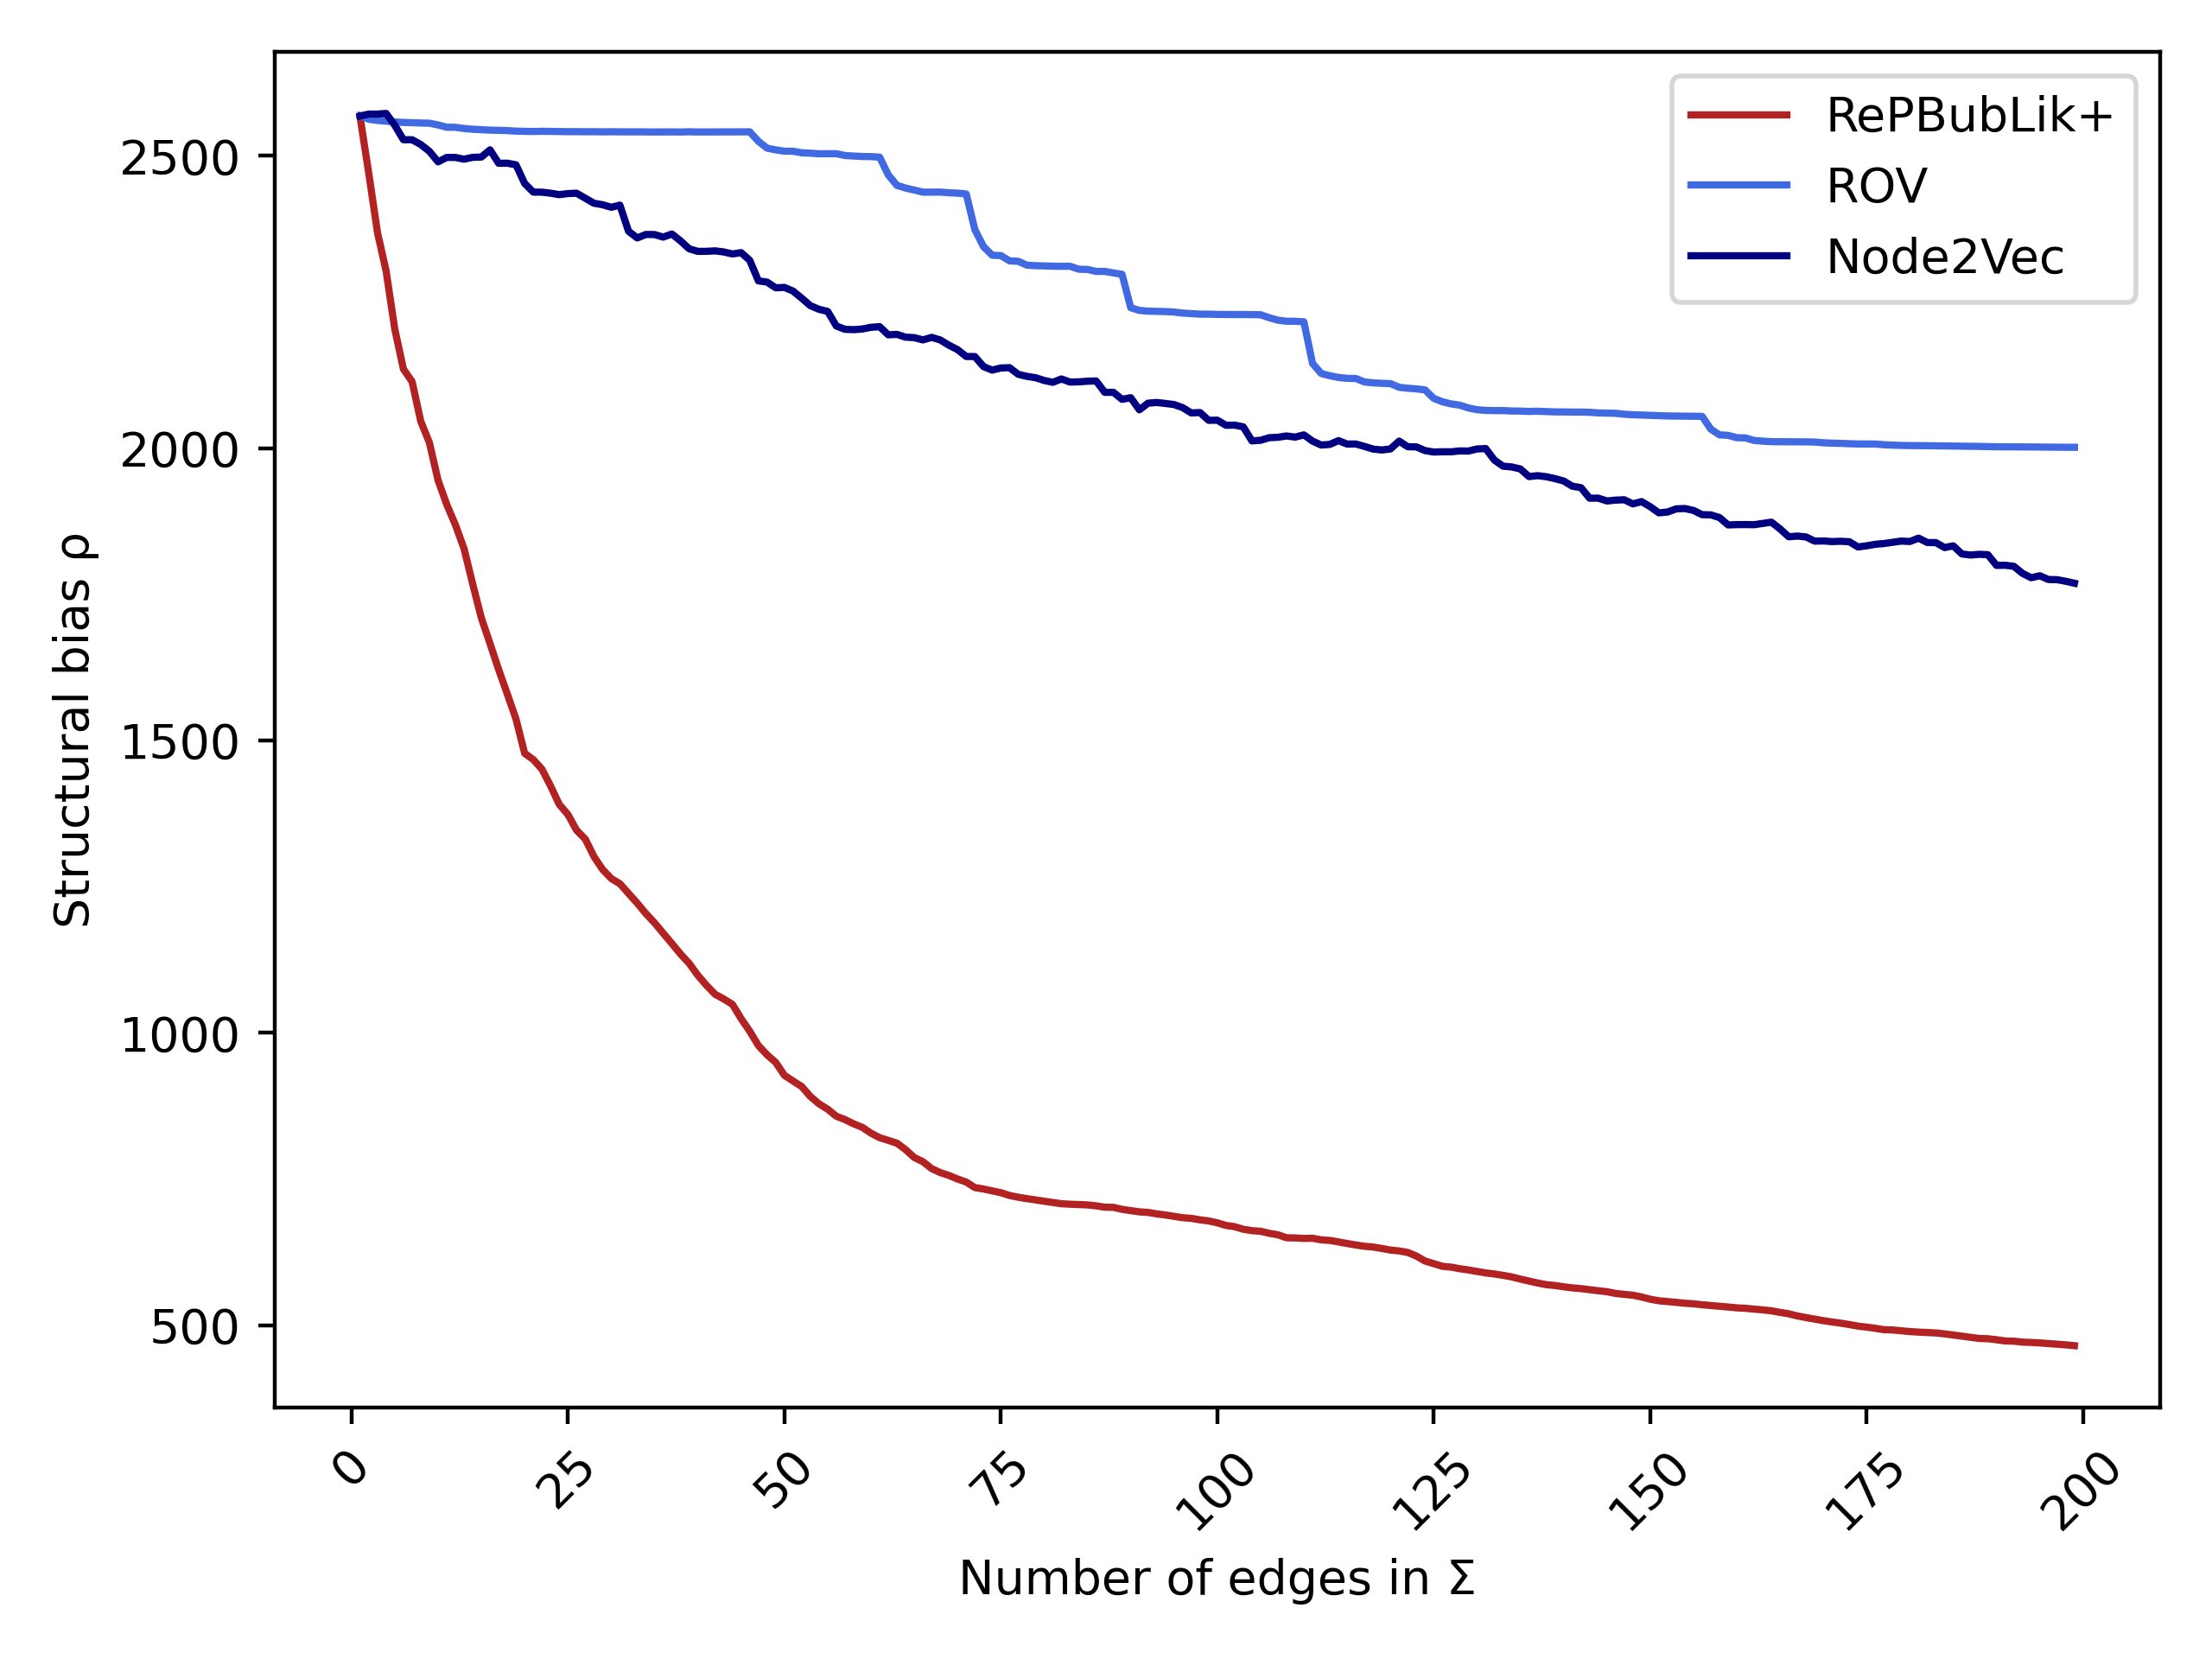
\includegraphics[width=\columnwidth]{10/math_ast_bias_10.png}
    \caption{\emph{MaA}s plot}\label{fig:maas_b_10}
\end{subfigure}
\hspace{0.1\columnwidth}
\begin{subfigure}[b]{0.4\textwidth}
    \centering
    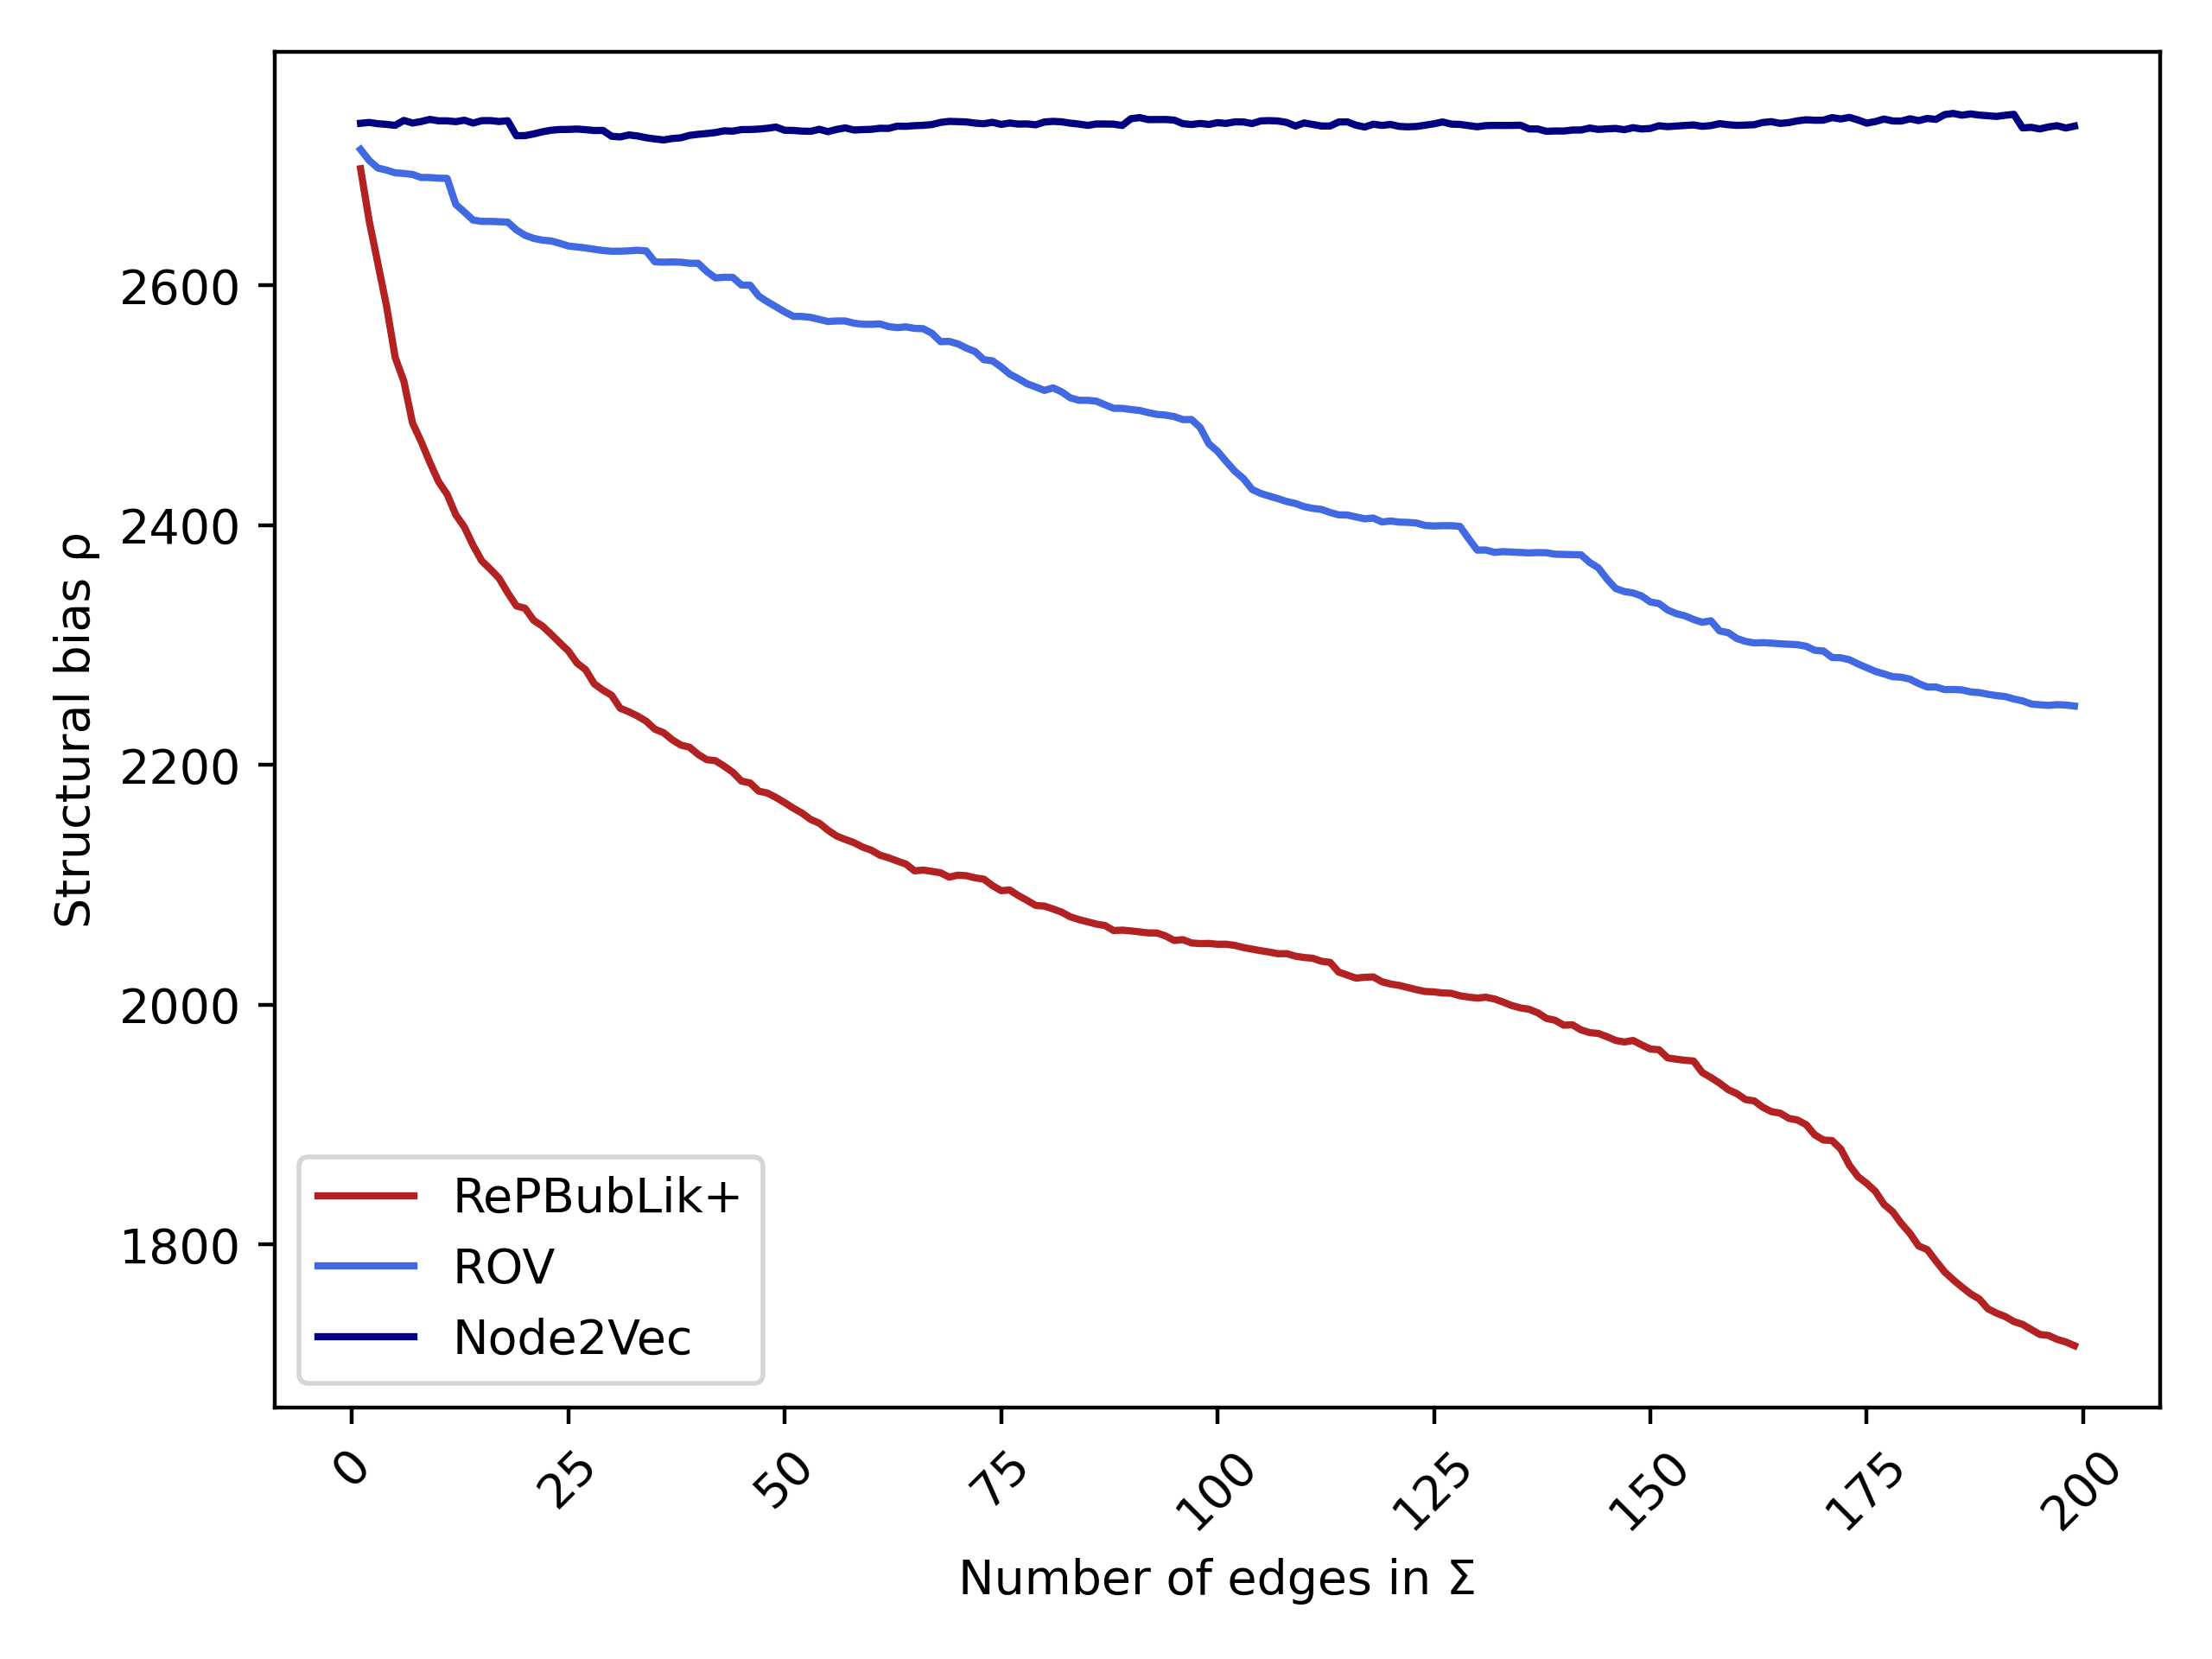
\includegraphics[width=\columnwidth]{10/polblogs_bias_10.png}
    \caption{\emph{PolBlogs} plot}\label{fig:polblogs_b_10}
\end{subfigure}
\caption{Grafici $\rho(G)$ per $t=10$}
\end{figure}
\newpage
\begin{figure}[!h]
    \centering
\begin{subfigure}[b]{0.4\textwidth}
    \centering
    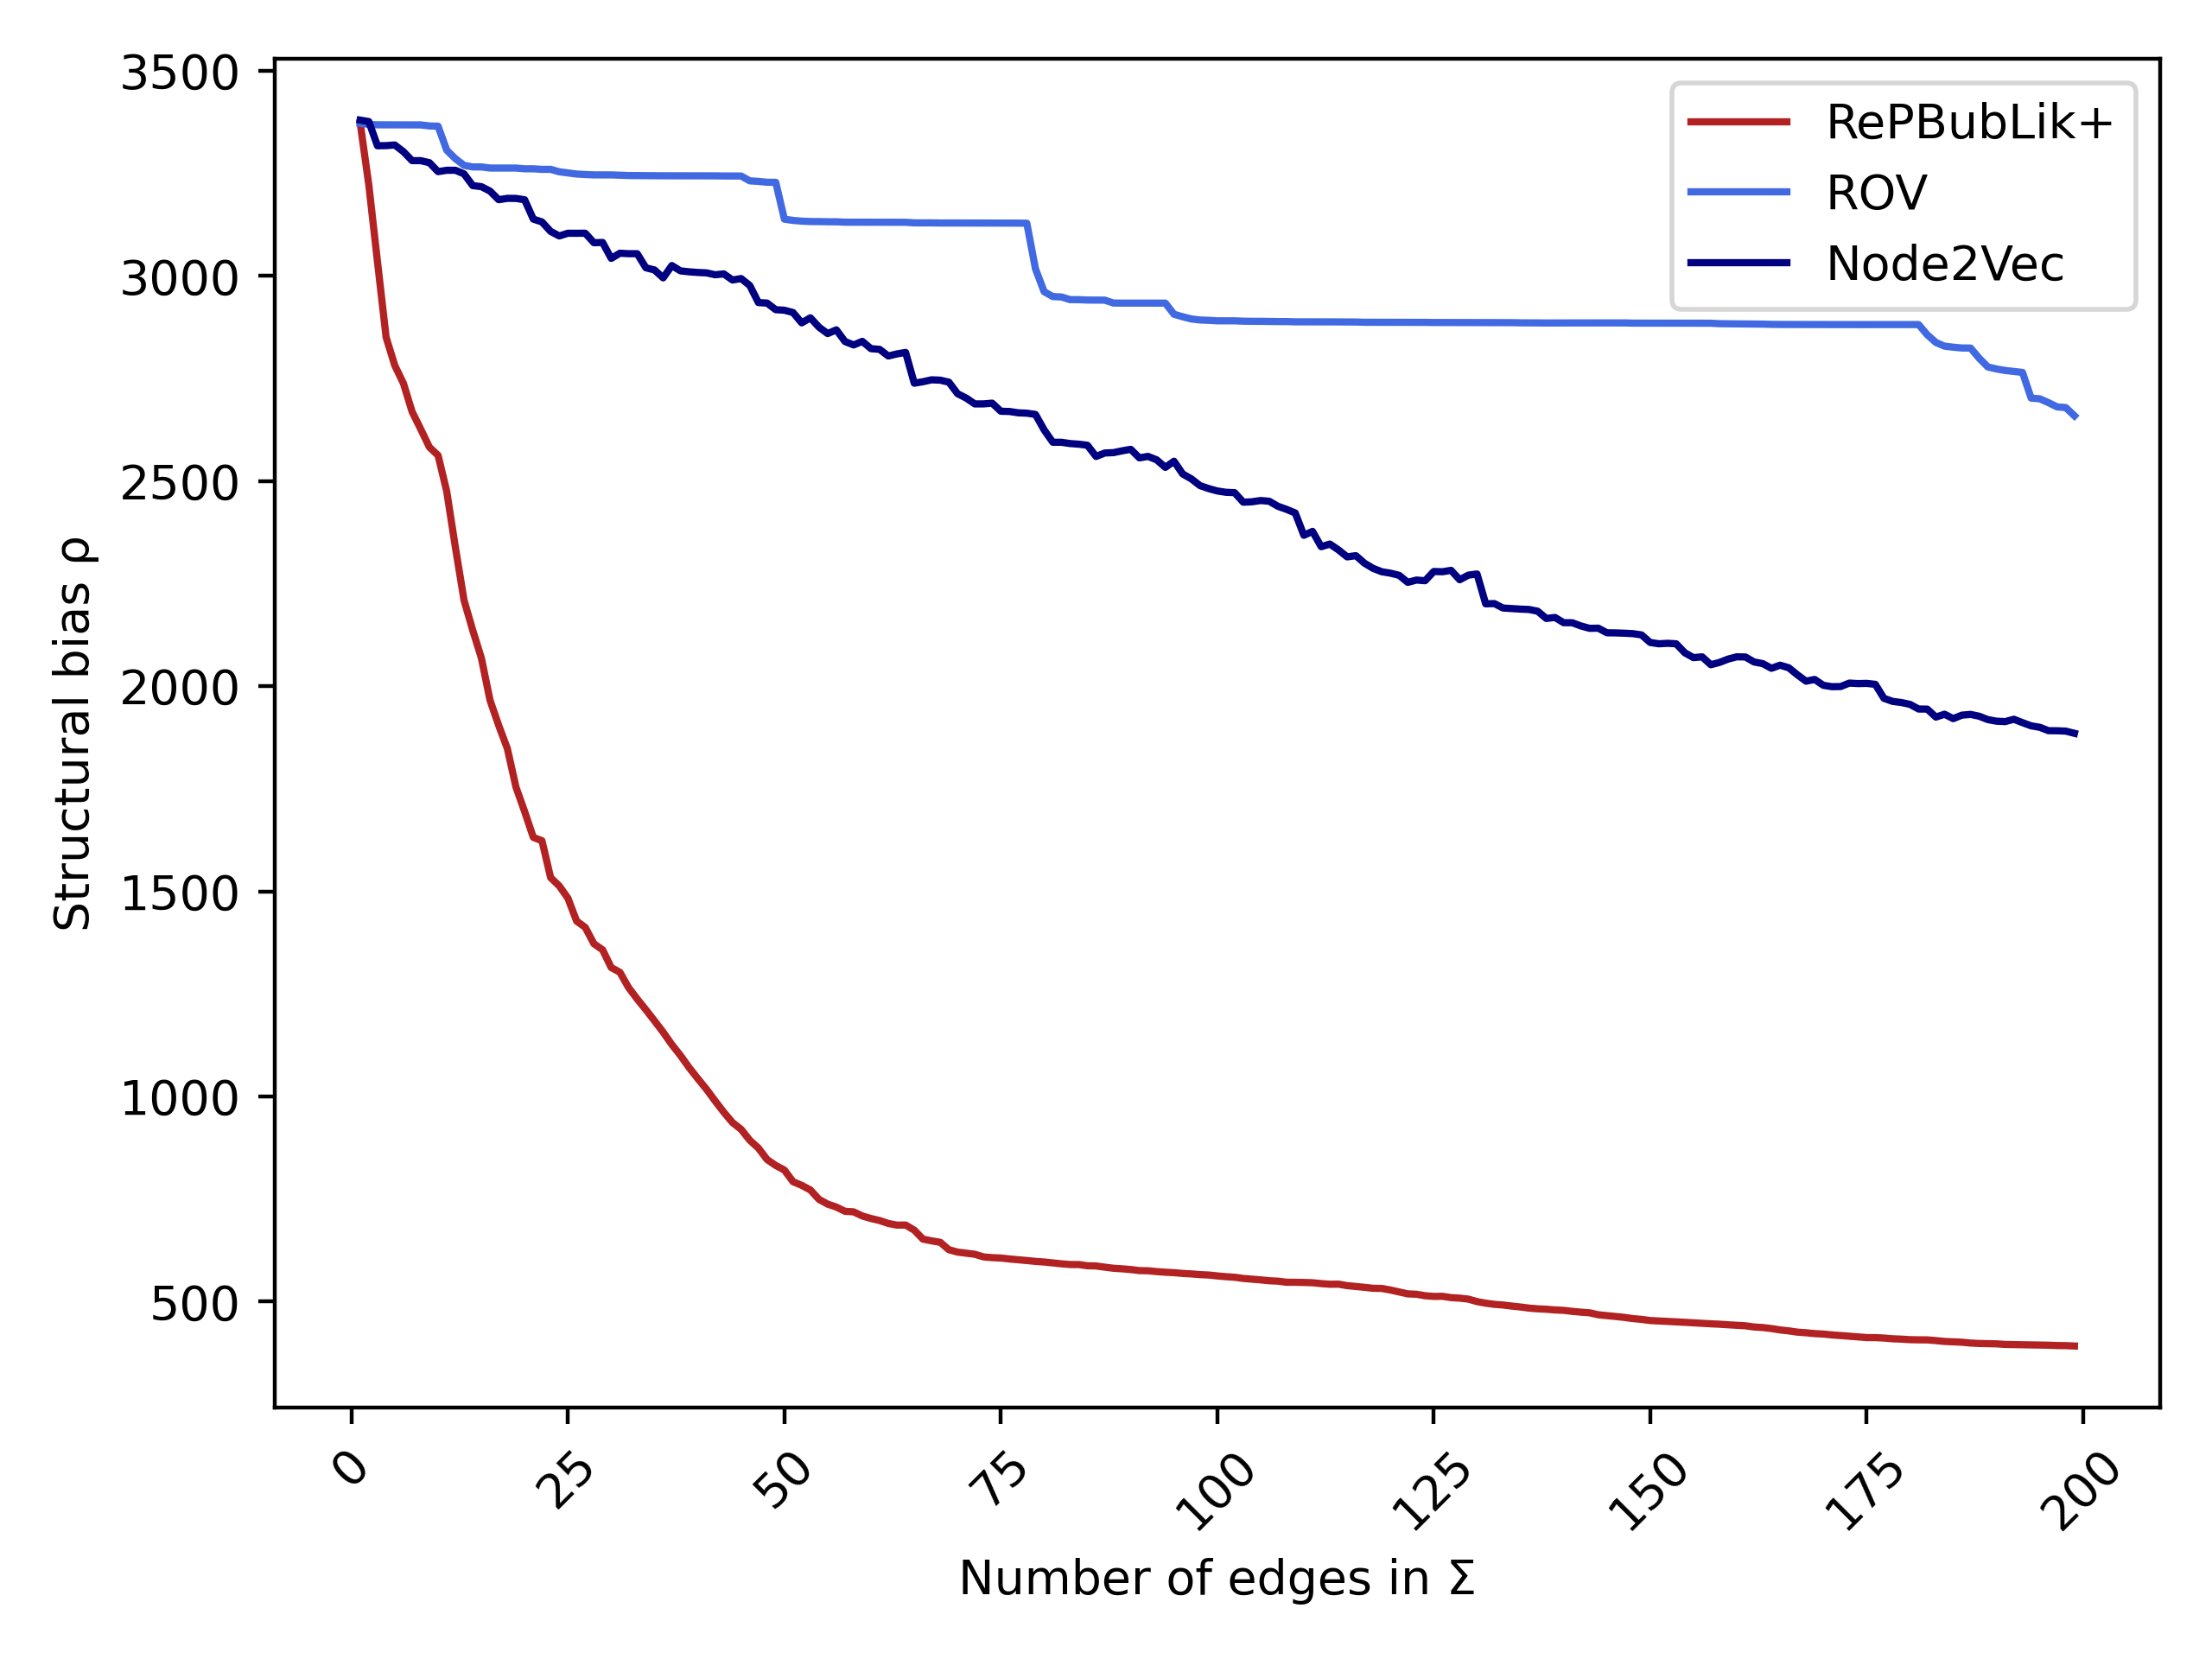
\includegraphics[width=\columnwidth]{15/math_tech_bias_15.png}
    \caption{\emph{MaTe} plot}\label{fig:mate_b_15}
\end{subfigure}
\hspace{0.1\columnwidth}
\begin{subfigure}[b]{0.4\textwidth}
    \centering
    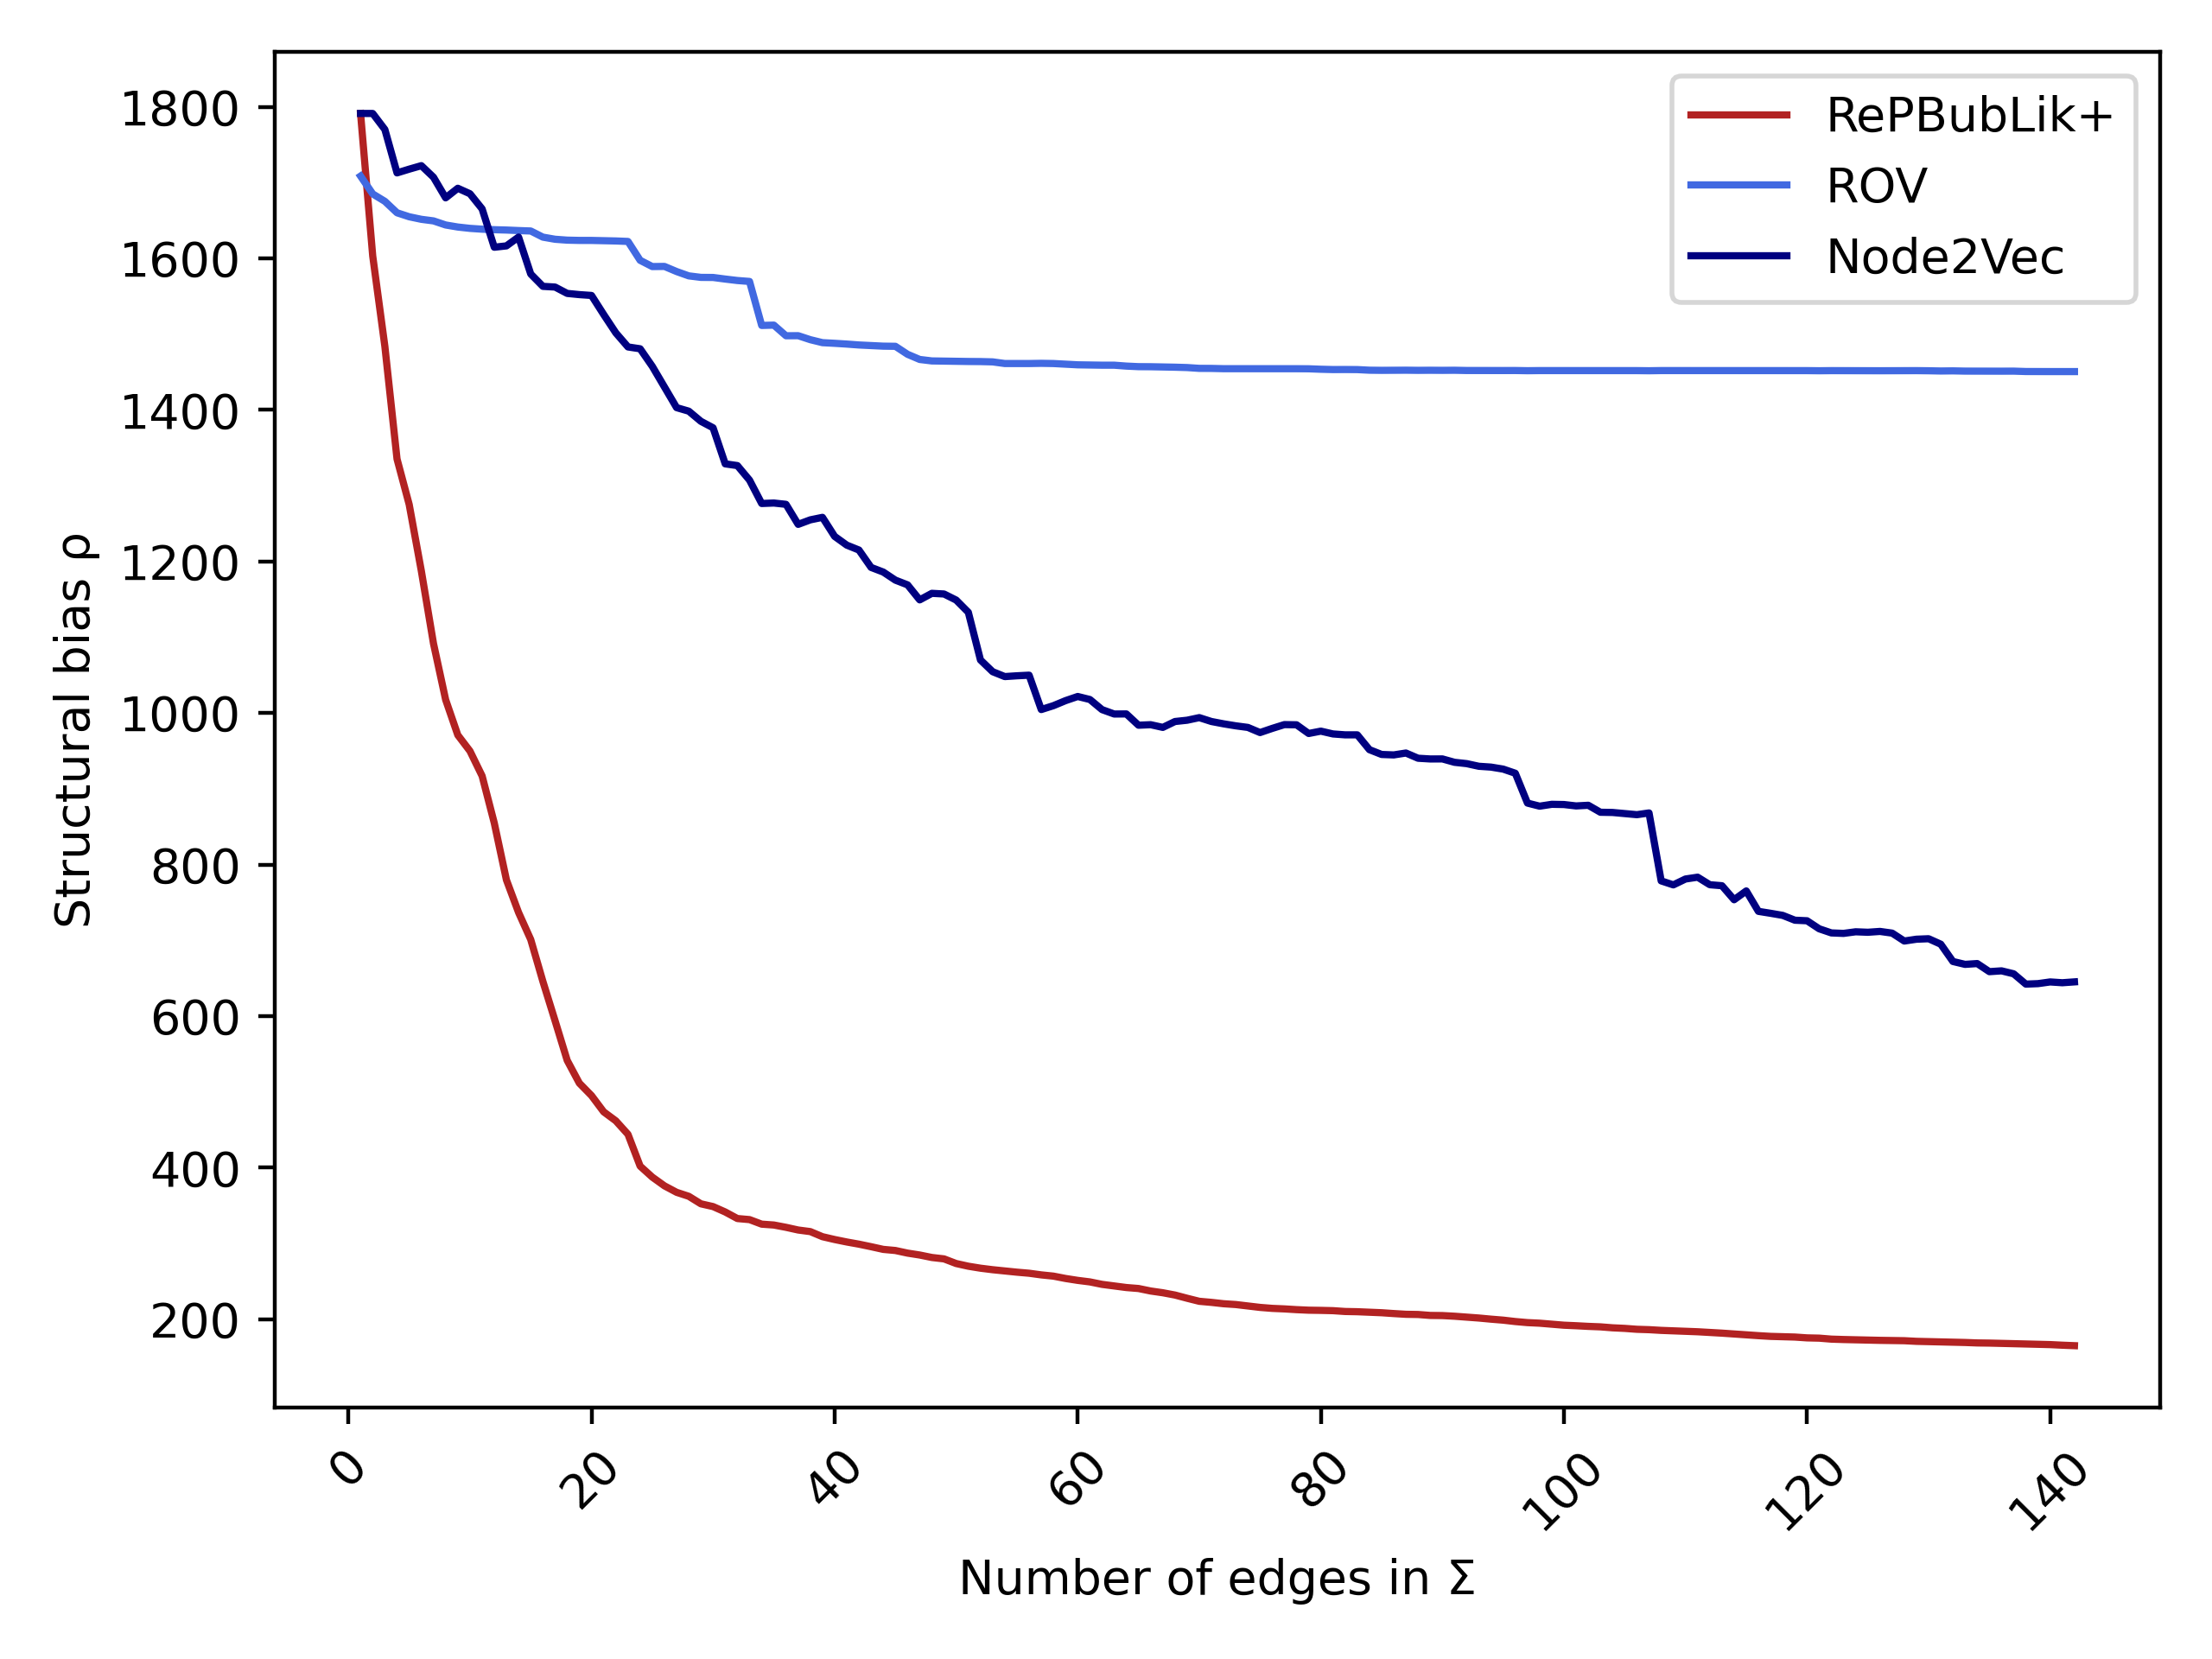
\includegraphics[width=\columnwidth]{15/tech_mil_bias_15.png}
    \caption{\emph{MiHi} plot}\label{fig:mihi_b_15}
\end{subfigure}

\begin{subfigure}[b]{0.4\textwidth}
    \centering
    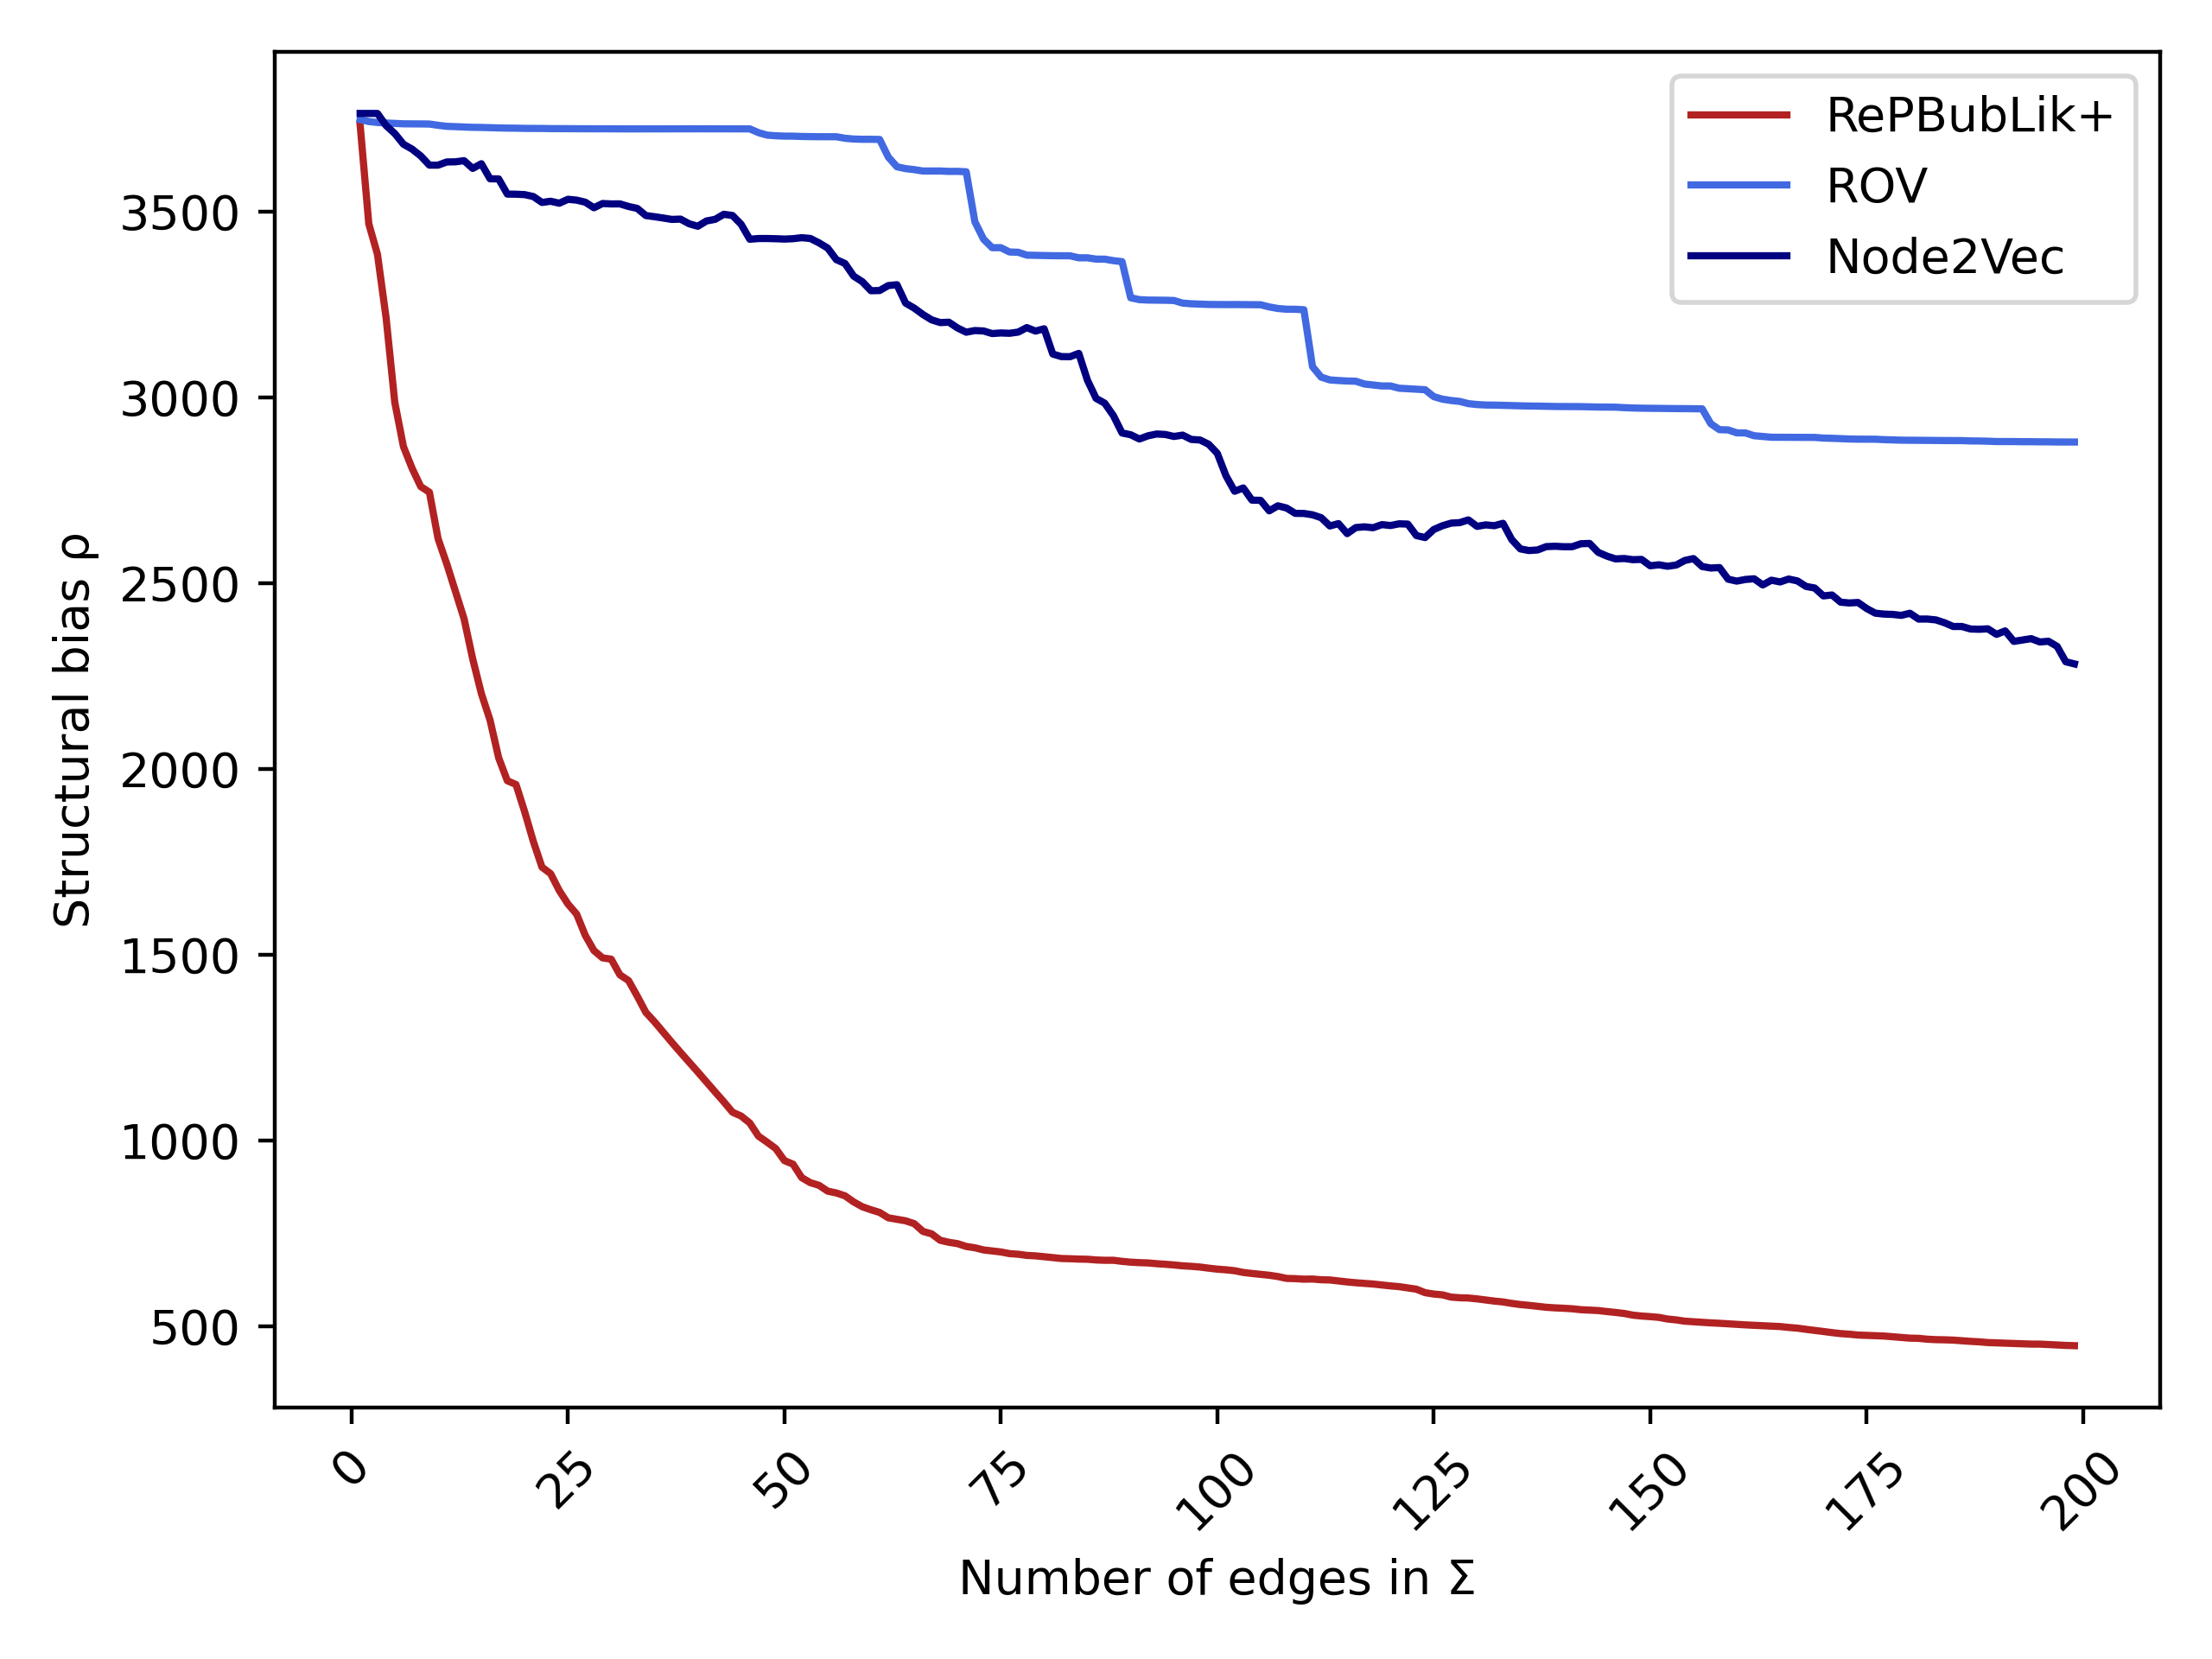
\includegraphics[width=\columnwidth]{15/math_ast_bias_15.png}
    \caption{\emph{MaA}s plot}\label{fig:maas_b_15}
\end{subfigure}
\hspace{0.1\columnwidth}
\begin{subfigure}[b]{0.4\textwidth}
    \centering
    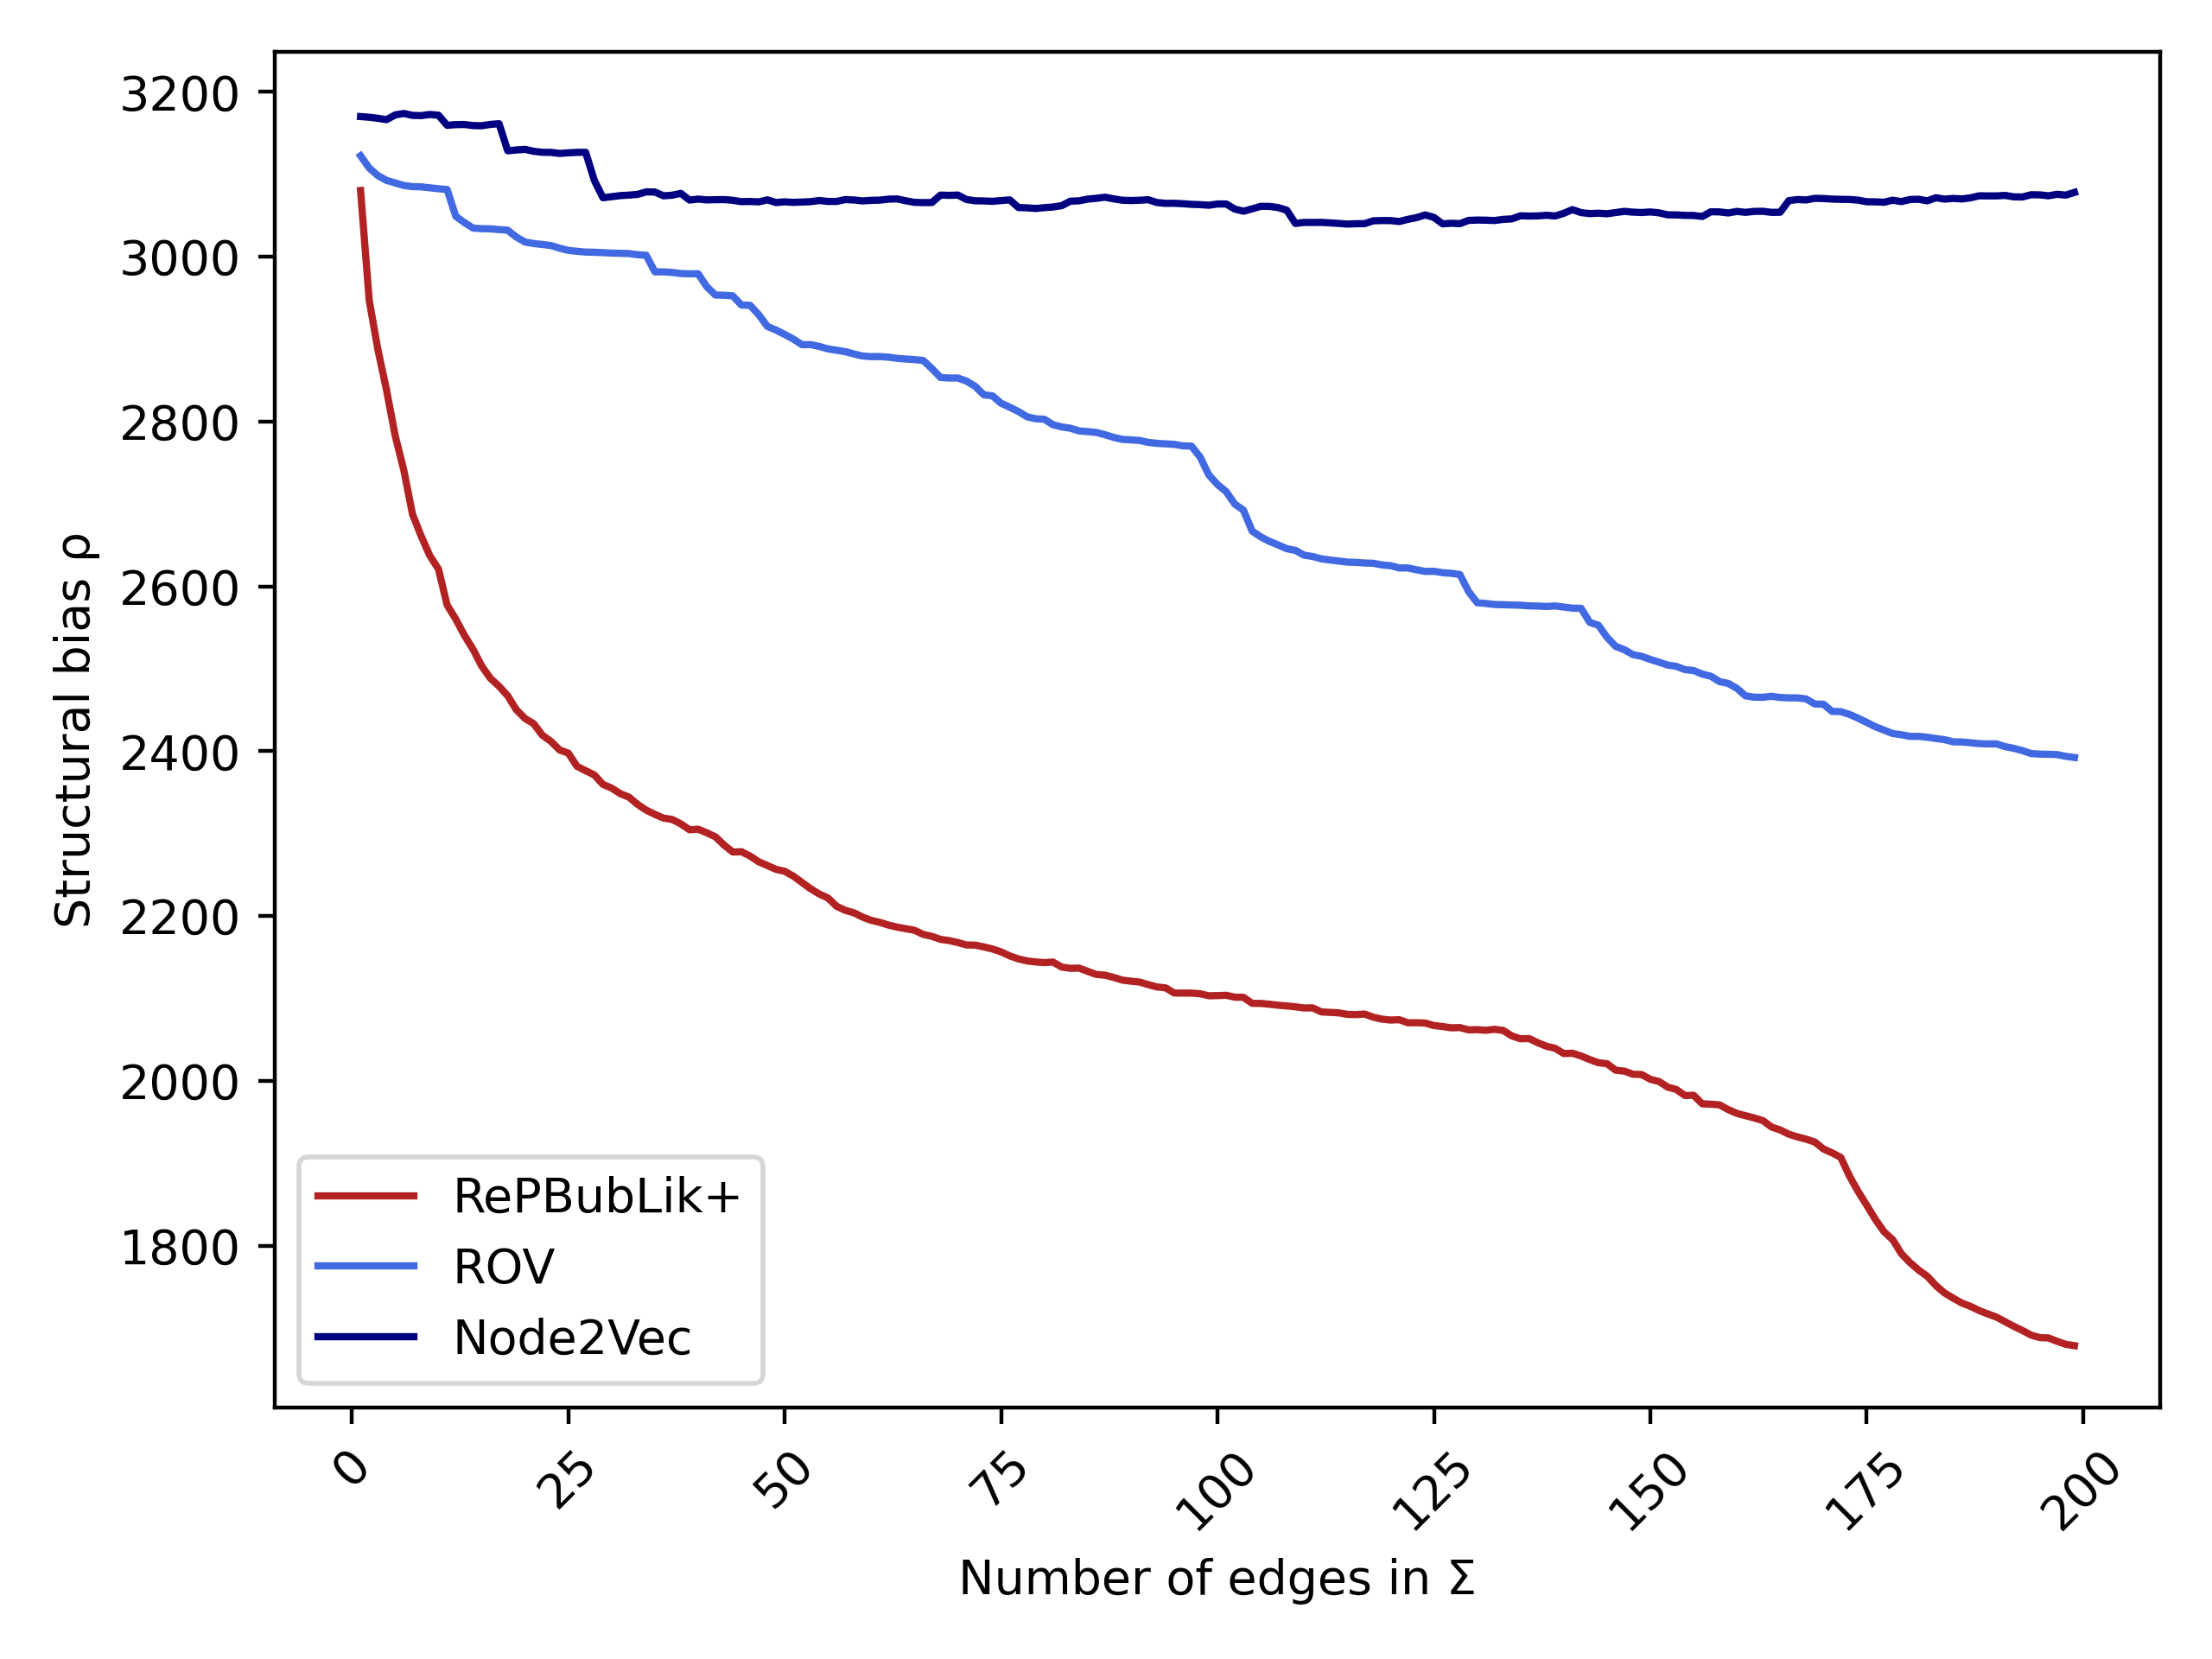
\includegraphics[width=\columnwidth]{15/polblogs_bias_15.png}
    \caption{\emph{PolBlogs} plot}\label{fig:polblogs_b_15}
\end{subfigure}
\caption{Grafici $\rho(G)$ per $t=15$}
\end{figure}
Dai grafici dei bias strutturali, si può dedurre che:
\begin{enumerate}
    \item RePBubLik+ è il migliore tra gli algoritmi proposti, in termini di riduzione di bias $\rho(G)$ rispetto al numero di archi in $\Sigma$.
    \item L'applicazione di RePBubLik+ a grafi di piccole dimensioni (\emph{MaTe}, \emph{MaAs}, \emph{MiHi}) porta ad una diminuzione del bias maggiore rispetto a quella ottenuta mediante gli algoritmi ROV e Node2Vec (es. (\emph{MaAs}) $\delta_{\rho_{R+}}=2700-480=2220$, $\delta_{\rho_{ROV}}=2700-2000=700$, ${\delta_{\rho_{Node2Vec}}}=2700-1800=900$ per $t=10$).
    \item L'applicazione di RePBubLik+ a grafi di medie dimensioni (\emph{PolBlogs}) porta ad una diminuzione del bias maggiore rispetto a quella ottenuta mediante gli algoritmi ROV e Node2Vec (es. (\emph{PolBlogs}) $\delta_{\rho_{R+}}=2750-1500=1250$, $\delta_{\rho_{ROV}}=2750-2250=500$, ${\delta_{\rho_{Node2Vec}}}=2750-2700=50$ per $t=10$).
    \item RePBubLik+ risulta essere il miglior algoritmo in quanto per un numero ridotto di archi riporta una notevole diminuzione del bias: nei grafici sovrastanti, la curva dell'algoritmo RePBubLik+ diminuisce molto rapidamente per valori piccoli di $k$, raggiungendo una plateau per un certo valore di $\rho(G)$.
            Questo, dal punto di vista pratico, è molto interessante perchè permette con pochi archi aggiuntivi di aumentare notevolmente la navigabilità in grafi simili a quelli presi in esame (es. (\emph{MaTe}) $\delta_{\rho_{R+}}=2300-760=1540$, $\delta_{\rho_{ROV}}=2300-2200=100$, ${\delta_{\rho_{Node2Vec}}}=2300-1900=400$ per $k=50,t=10$).
    \item Le considerazioni fatte nei punti precedenti sono generalmente valide, per qualsiasi valore di $t$ e qualsiasi grafo. Valutando il bias strutturale dei grafi anche in termini di RW massimo, si può notare che per valori di $t$ maggiori, RePBubLik+ raggiunge il plateau con un numero inferiore d'archi (es. (\emph{MaTe}) $\delta_{\rho_{R+}}=1350-675=675$ per $k=50, t=5$,  $\delta_{\rho_{R+}}=2300-760=1540$ per $k=50,t=10$, $\delta_{\rho_{R+}}=3400-800=2600$ per $k=50,t=15$).
\end{enumerate}

\subsection{Conclusioni}
Considerando tutti i dati ottenuti dagli esperimenti svolti, RePBubLik+ risulta essere il miglior algoritmo in termini di rapporto tra guadagno e tempo impiegato.
Le performance di quest'ultimo, infatti, variano notevolmente a seconda dei parametri forniti: per valori di $t$ maggiori, 
il guadagno, e la conseguente diminuzione del bias strutturale, aumentano significativamente, a discapito dei tempi di esecuzione. 
Sarebbe utile, quindi, determinare quale lunghezza massima di RW meglio si addice ad un determinato grafo e quanto sia importante la diminuzione della polarizzazione in quella rete.
Per valutare al meglio le performance di RePBubLik+, un'analisi su dataset di dimensioni notevolmente maggiori permetterebbe di esaminare quanto il volume della rete
influenzi le performance dell'algoritmo. 





% %\afterpage{\blankpage}

% % Chapter 5
% \clearpage{\pagestyle{plain}\cleardoublepage}
% \chapter{Conclusioni}
% Questa tesi presenta diversi approcci per la riduzione della polarizzazione nella navigazione nei grafi, ovvero gli algoritmi RePBubLik e ShuffLik.
RePBubLik permette di calcolare un'approssimazione accurata per il problema della riduzione del \emph{structural bias}.
In seguito alle considerazioni teoriche, son stati svolti dei confronti tra RePBubLik+, la versione più veloce e pratica dell'
algoritmo RePBubLik, e le attuali tecniche per la riduzione della polarizzaione dei grafi: ROV e 
Node2Vec. Dalle analisi, è emerso che RePBubLik+ permette di ridurre drasticamente il \emph{structural bias} 
del grafo con un numero di archi significativamente inferiore, rispetto agli altri approcci utilizzati. 
\\
In aggiunta, è stata brevemente descritta un tecnica alternativa a RePBubLik, che permette di aumentare
la navigabilità di una rete effettuando \emph{edge swapping}. 
Questo algoritmo prende il nome di ShuffLik ed esiste una sua versione più pratica, ShuffLik+.
Importante notare che ShuffLik risulta efficace in contesti dove non è possibile eseguire \emph{edge inserction} per motivi di costo o di vincoli funzionali, 
operando quindi interventi meno invasivi.
\\
Possiamo osservare diverse opportunità di sviluppo futuro:
\begin{enumerate}
    \item Nella pratica, potrebbe essere difficile stimare le probabilità di transizione all'interno del grafo. I pesi da assegnare agli archi potrebbero 
    essere appresi mediante un algoritmo di machine learning sui dataset.
    \item La determinazione di valori realistici del parametro $t$ non è semplice. È un problema rilevante individuare il valore ideale di random walk da fornire all'algoritmo, in funzione del trade-off tra guadagno e tempo di esecuzione.
    \item Nell'estensione a più ``colori'' dell'algoritmo, diventa importante determinare quale coppia di ``colori'' permette, con un numero ridotto ti archi, di ridurre notevolmente il bias strutturale.
\end{enumerate} 

% %\afterpage{\blankpage}

% % Bibliography
% \clearpage{\pagestyle{plain}\cleardoublepage}

% 
\begin{thebibliography}{9}
    \bibitem{RePBubLik+&ShuffLik}
    Shahrzad Haddadan, Cristina Menghini, Matteo Riondato, Eli Upfal (2022) \emph{Reducing polarization and increasing diverse navigability in graphs by inserting edges and swapping edge weights. In Proceedings of ACM WSDM'21.}
    \href{https://link.springer.com/article/10.1007/s10618-022-00875-8}{\url{https://link.springer.com/article/10.1007/s10618-022-00875-8}}
    
    \bibitem{Github}
    Cristina Menghini (2021) \emph{Reducing Polarization and Improving Diverse Navigability}
     \href{https://github.com/CriMenghini/RePBubLik}{\url{https://github.com/CriMenghini/RePBubLik}}
    
    \bibitem{Amazon}
    Amazon (2006) \emph{Amazon product co-purchasing network metadata.}
    \href{https://snap.stanford.edu/data/amazon-meta.html}{\url{https://snap.stanford.edu/data/amazon-meta.html}}
    
    \bibitem{PolBlogs}
    PolBlogs (2005) \emph{A directed network of hyperlinks between weblogs on US politics.}
    \href{http://www-personal.umich.edu/~mejn/netdata/}{\url{http://www-personal.umich.edu/~mejn/netdata/}} 
    
    \bibitem{ROV}
    Kiran Garimella, Gianmarco De Francisci Morales, Aristides Gionis, and Michael Mathioudakis (2017) \emph{Reducing Controversy by Connecting Opposing Views. In Proceedings of the Tenth ACM International Conference on Web Search and Data Mining (WSDM'17).}
    \href{https://arxiv.org/abs/1611.00172}{\url{https://arxiv.org/abs/1611.00172}}

    \bibitem{Node2Vec}
    Aditya Grover, Jure Leskovec (2016) \emph{node2vec: Scalable feature learning for networks. In Proceedings of the 22nd ACM SIGKDD international conference on Knowledge discovery and data mining.}
    \href{https://cs.stanford.edu/~jure/pubs/node2vec-kdd16.pdf}{\url{https://cs.stanford.edu/~jure/pubs/node2vec-kdd16.pdf}}
    
    \bibitem{Grafo}
    Wikipedia (2023) \emph{Graph theory}
    \href{https://en.wikipedia.org/wiki/Graph_theory}{\url{https://en.wikipedia.org/wiki/Graph_theory}}

    \bibitem{RWCC}
    Wikipedia (2022) \emph{Random walk closeness centrality}
    \href{https://en.wikipedia.org/wiki/Random_walk_closeness_centrality}{\url{https://en.wikipedia.org/wiki/Random_walk_closeness_centrality}}
\end{thebibliography}



% \clearpage{\pagestyle{plain}\cleardoublepage}
% \chapter*{Ringraziamenti}
% Al termine di questa tesi, voglio ringraziare di cuore tutti coloro che in questi tre anni 
hanno contribuito, nel bene o nel male, alla mia crescita personale e universitaria. 
\\
In primo luogo, voglio ringraziare il mio relatore, Leonardo Pellegrina, per la pazienza e il 
tempo dedicatomi durante la stesura della tesi. Inoltre, desidero ringraziare Cristina Menghini, 
senza la quale non avrei potuto completare una buona parte della tesi.
\\ 
Oltre ai ringraziamenti accademici, desidero ringraziare tutti coloro che in questi anni mi hanno aiutato a
crescere come persona, oltre che a sostenermi nei momenti di difficoltà: Modolo, Zanzi, Zinca, Sheldon, Colla e Kabir. 
Senza di voi questi tre anni accademici non sarebbero passati così velocemente. 
\\
Non meno importanti, voglio ringraziare tutti i miei compagni di karate: Giacomo, Elia, Nicola, Beatrice, 
Giada, Mauro e la mia allenatrice Alice. 
Anche se, sfortunatamente, non ci vediamo più con la stessa periodicità di un tempo, sarete sempre 
la mia seconda famiglia: mi avete insegnato la disciplina e la perseveranza, qualità senza le quali non
sarei dove sono ora.
\\ 
Per ultimi, ma non per importanza, voglio ringraziare la mia famiglia, in particolare mia madre Roberta
e mio padre Davide. Anche se spesso non lo dimostro, siete fondamentali nella mia vita. Oltre a sfamarmi 
e viziarmi, mi avete sempre dimostrando molta fiducia, sostenendomi in ogni mia scelta. 
Per questo e per mille altri motivi, voglio ringraziarvi dal profondo del mio cuore.
\\ 
In conclusione, ringrazio nuovamente ogni persona citata per avermi sostenuto e aver creduto in me. 
Quest'oggi voglio condividere con voi questo mio traguardo.
Un traguardo che non è un punto di arrivo, bensì la partenza di un nuovo inizio, dove desidero avervi al mio fianco!\\
\emph{Memento audere semper}


\end{document}